\chapter{Appendix A} \label{ch:appendices}

\section{Capgemini server dataset}\label{appendices:serverdata}

This section serves as a complete overview of the data. The server data that is provide by Capgemini has been developed by their own developers and as such contains a custom schema. Event logs contain multiple columns shown in table \ref{tab:tableservercol} in an order fashion. Due to privacy reason, we will not show the data that is contained within the rows. Only two columns are worth discussing: syslog.body, syslog.severity. The former contained a lot of server specific data. This event log has been formatted to have a lot in common with the syslog message standard. The latter contains the type of message the event log, e.g. 0 indicating an emergency message. Due to a formatting error discovered during the research, the original syslog.severity has been lost and is always labelled 6 meaning informational. 

\begin{table}[h]
\centering
 \begin{tabular}{|l|l|l|l|l|l|} 
 \hline
 filename & hostname & mime.type & path & syslog.body & syslog.facility \\ [0.5ex] 
 \hline\hline
 syslog.hostname & syslog.port & syslog.priority & syslog.protocol & syslog.sender & syslog.severity  \\ [0.5ex]
 \hline\hline
 syslog.timestamp & syslog.valid & syslog.version & timestamp & uuid & \\
 \hline
 \end{tabular}
\caption{All the columns in the complete dataset}
\label{tab:tableservercol}
\end{table}

After manually inspecting the data we extracted only 4 columns named: hostname, uuid, syslog.body, timestamp. A custom solution had to be written to transform the servers logs into a use able matrix. These steps are explained in section \ref{methodology:dataset}. 

\FloatBarrier

\section{pyLDAvis}\label{appendices:pyldavis}

 \begin{figure}[!h]
    \centering
    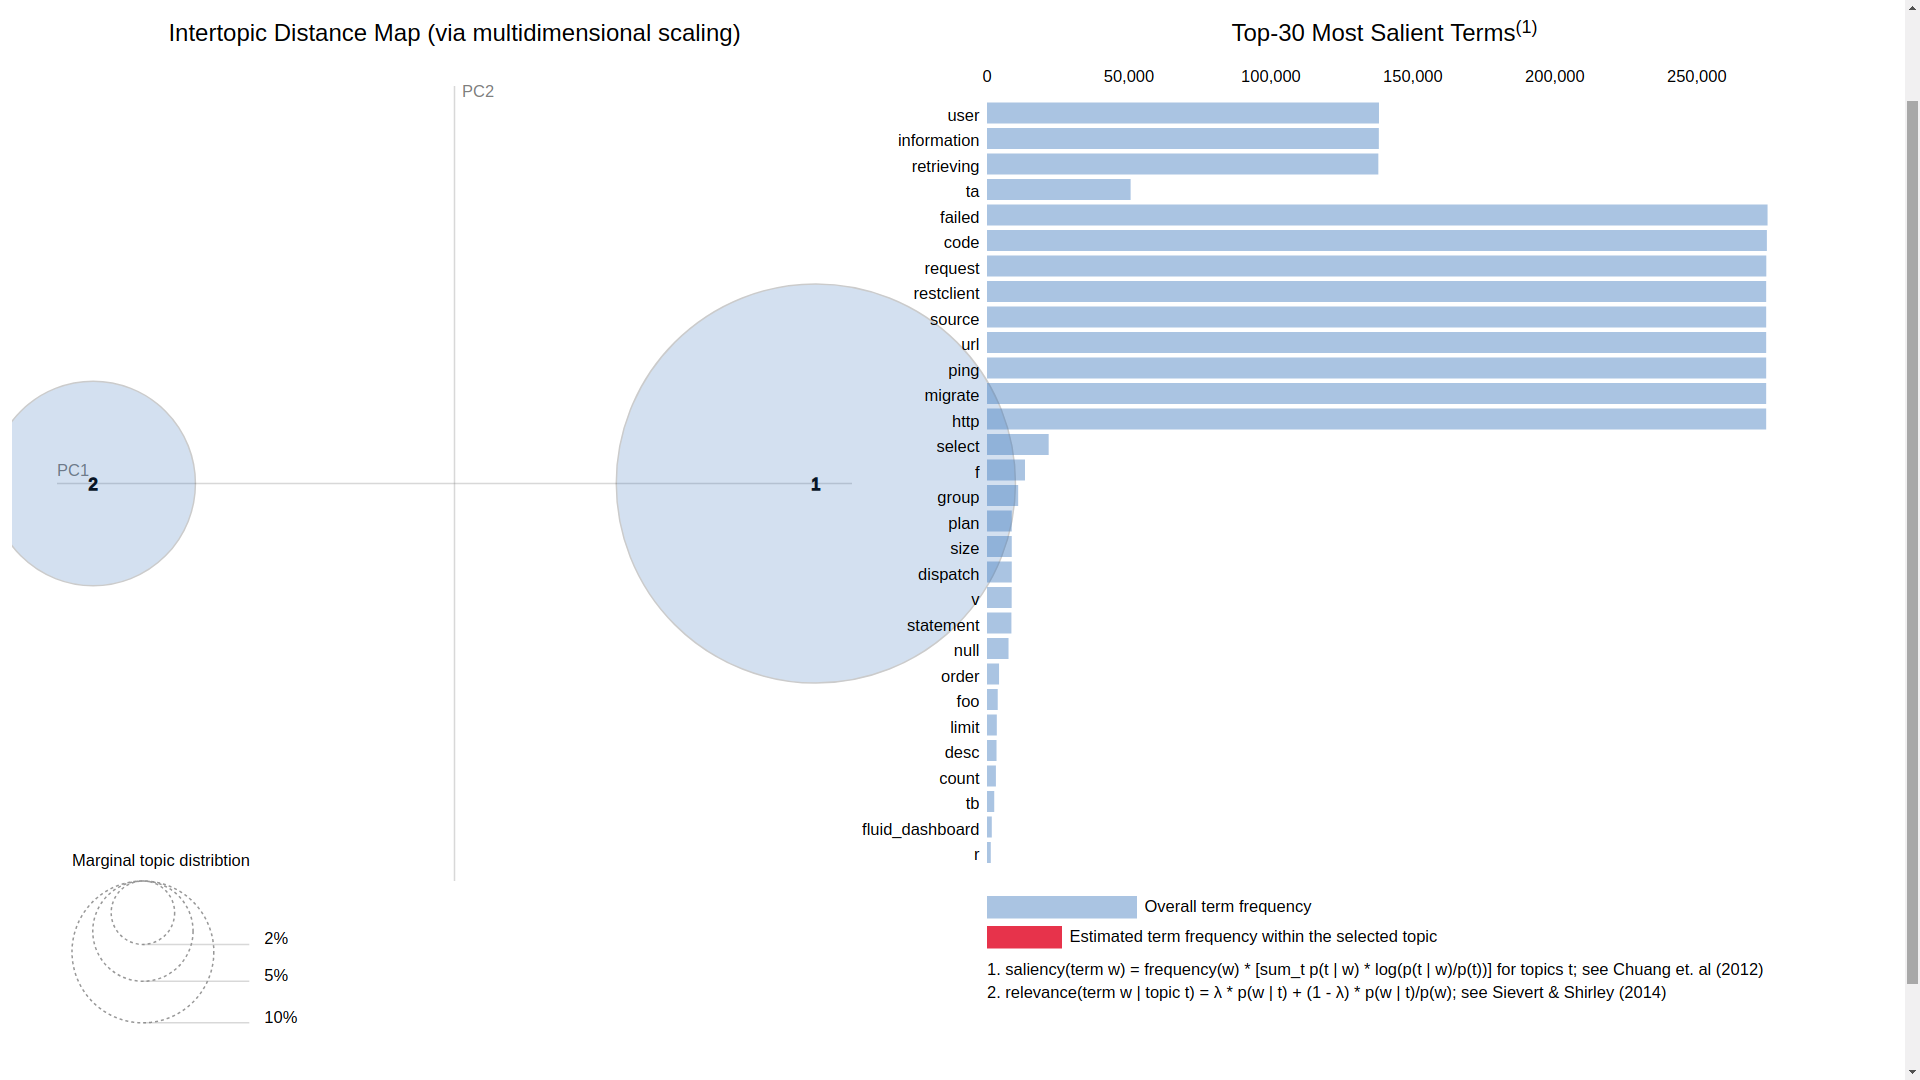
\includegraphics[width=15cm, height=8cm,trim=0 0 100px 0, clip=true]{figures/pyldavis/pyldavis_2.png}
    \caption{PyLdavis topic visualisation with 2 topics}
    \label{fig:pyldavis_2}
\end{figure}

 \begin{figure}[!h]
    \centering
    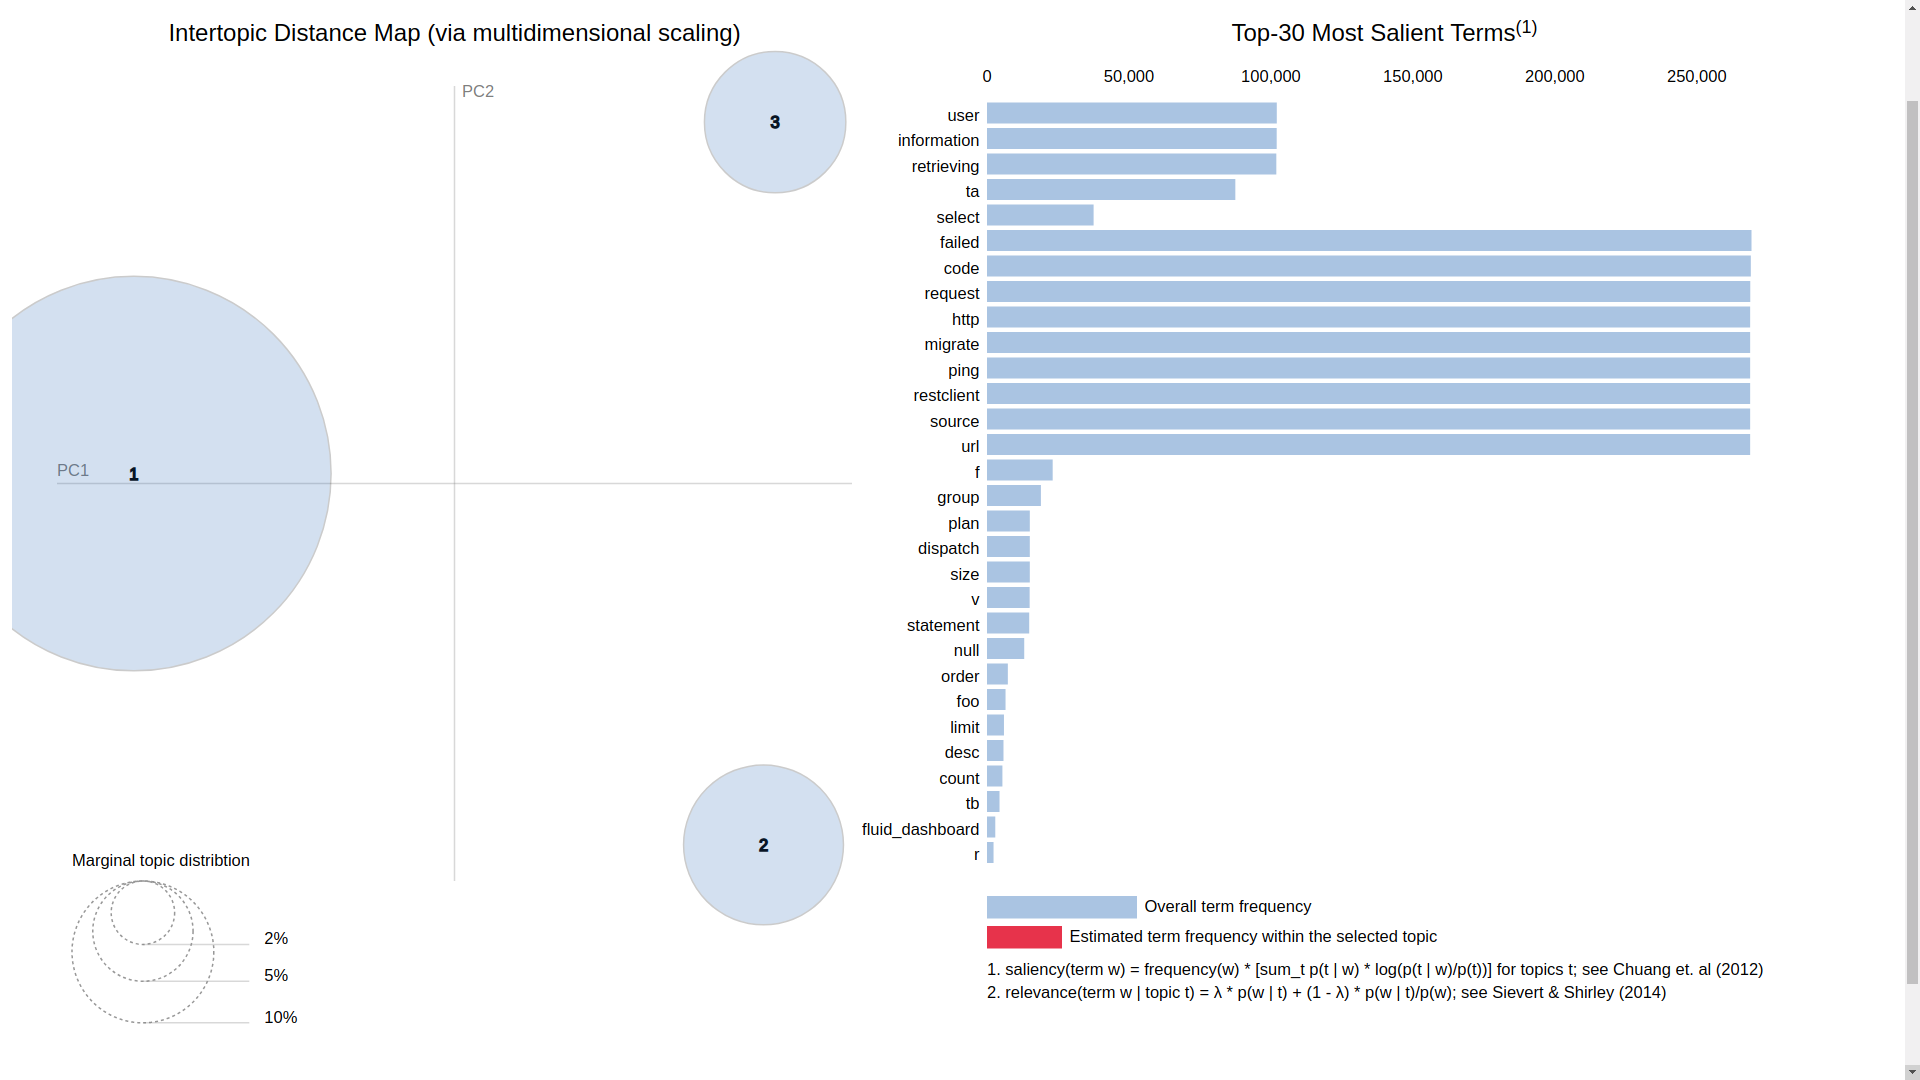
\includegraphics[width=15cm, height=8cm,trim=0 0 100px 0, clip=true]{figures/pyldavis/pyldavis_3.png}
    \caption{PyLdavis topic visualisation with 3 topics}
    \label{fig:pyldavis_3}
\end{figure}

 \begin{figure}[!h]
    \centering
    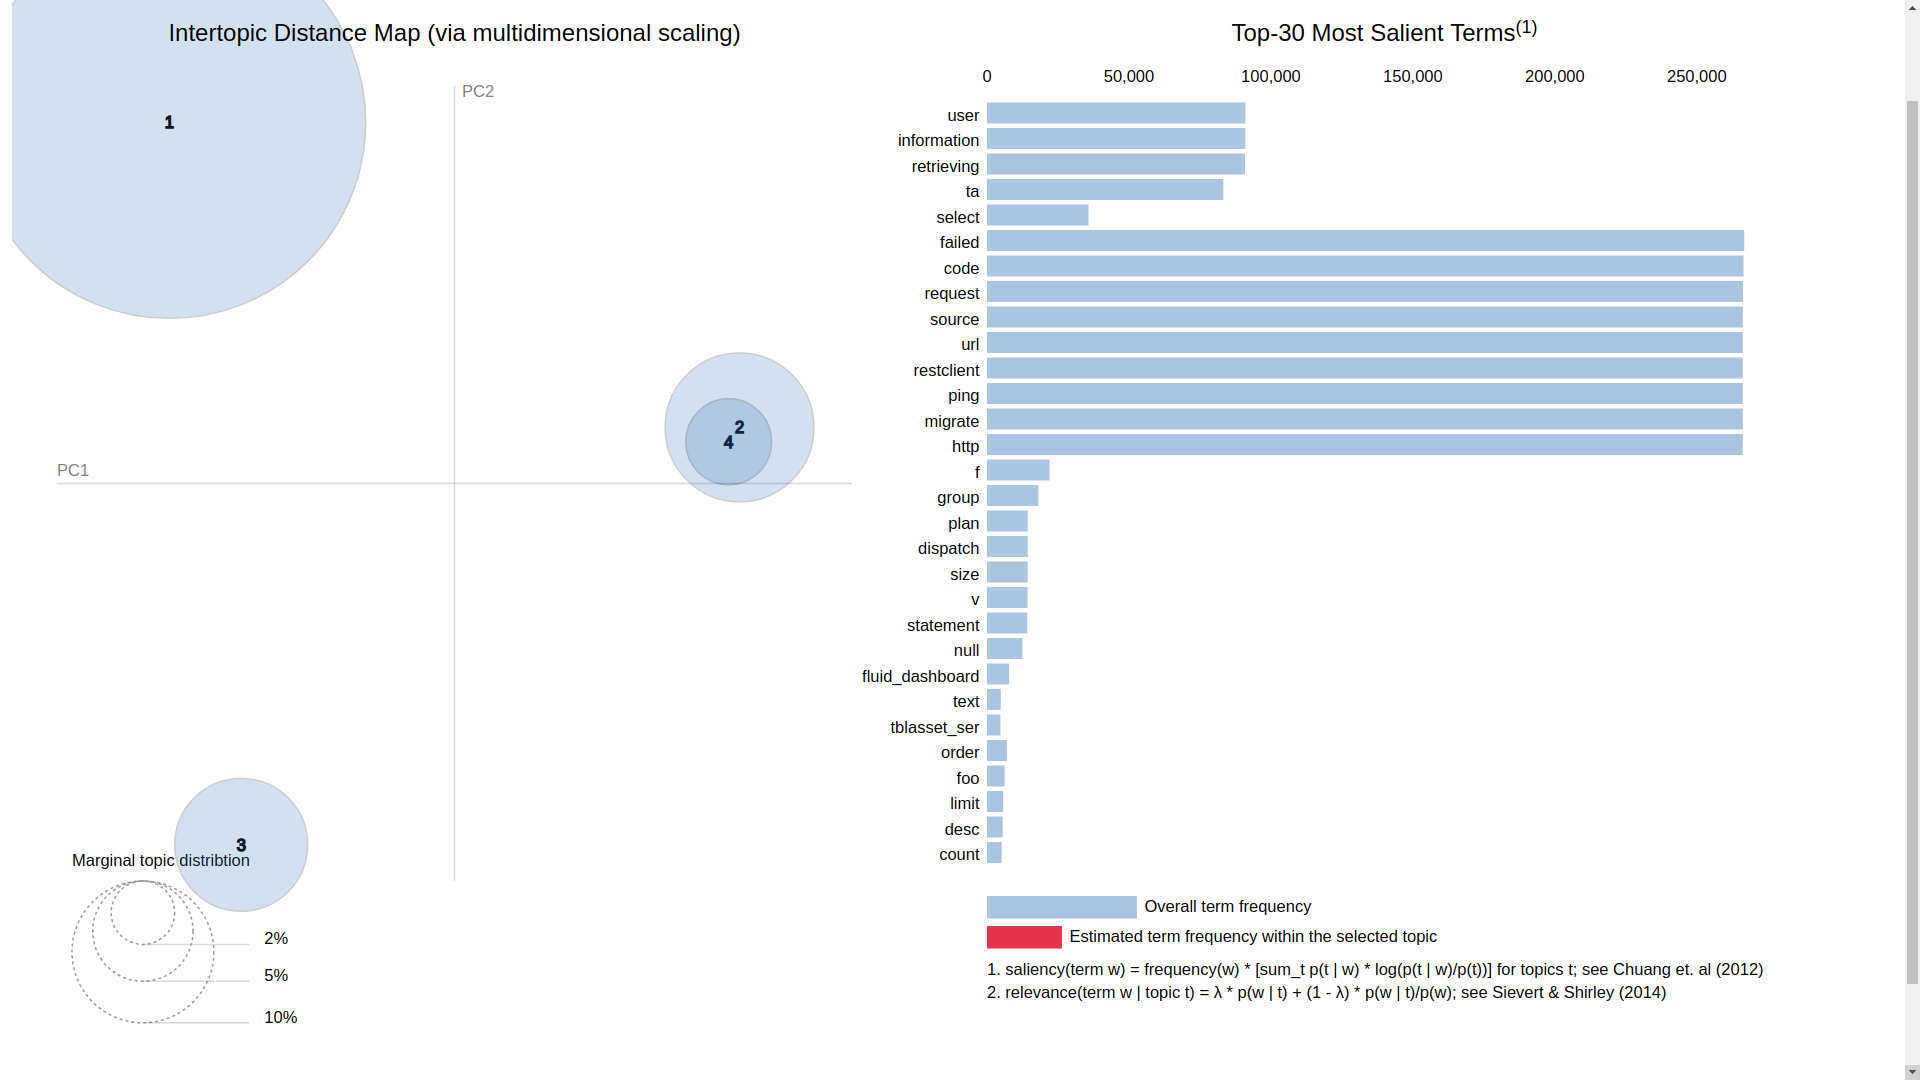
\includegraphics[width=15cm, height=8cm,trim=0 0 100px 0, clip=true]{figures/pyldavis/pyldavis_4.png}
    \caption{PyLdavis topic visualisation with 4 topics}
    \label{fig:pyldavis_4}
\end{figure}

  \begin{figure}[!h]
    \centering
    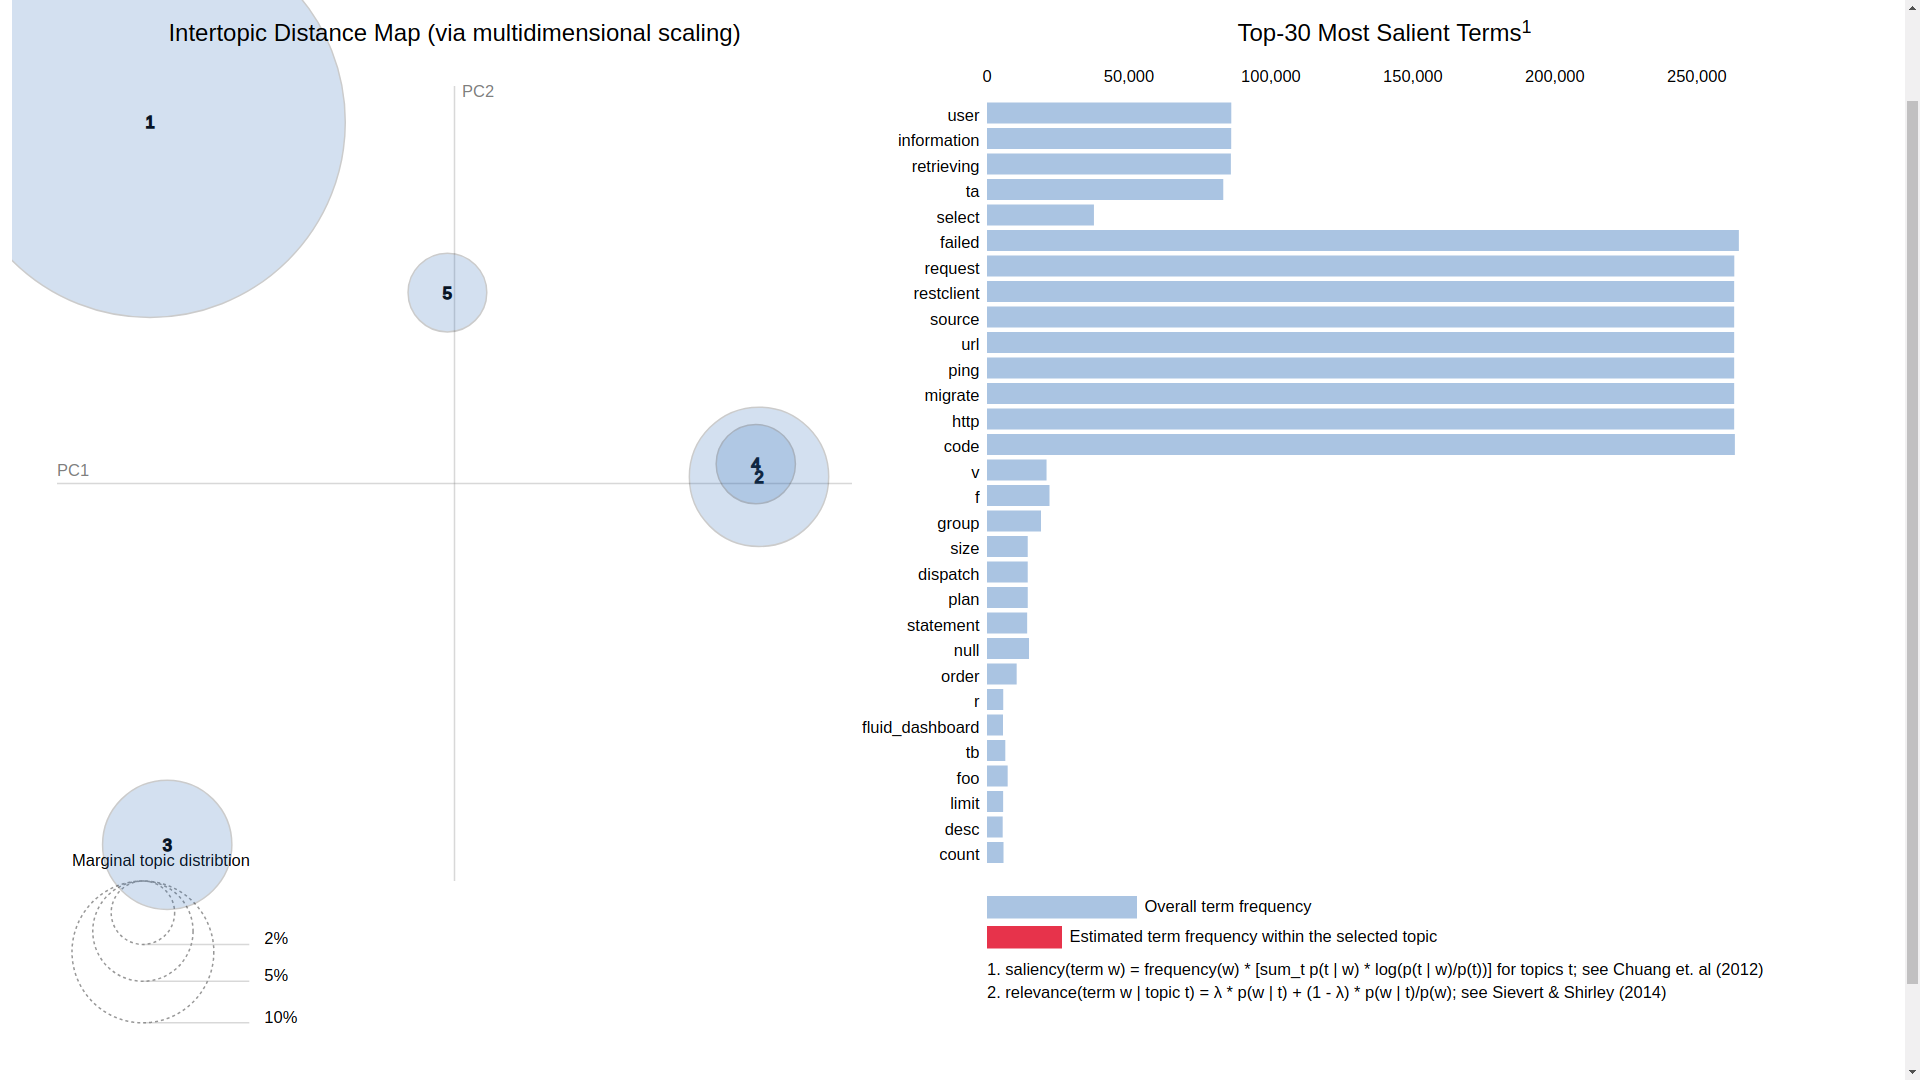
\includegraphics[width=15cm, height=8cm,trim=0 0 100px 0, clip=true]{figures/pyldavis/pyldavis_5.png}
    \caption{PyLdavis topic visualisation with 5 topics}
    \label{fig:appendices:pyldavis_5}
\end{figure}
 
 \begin{figure}[!h]
    \centering
    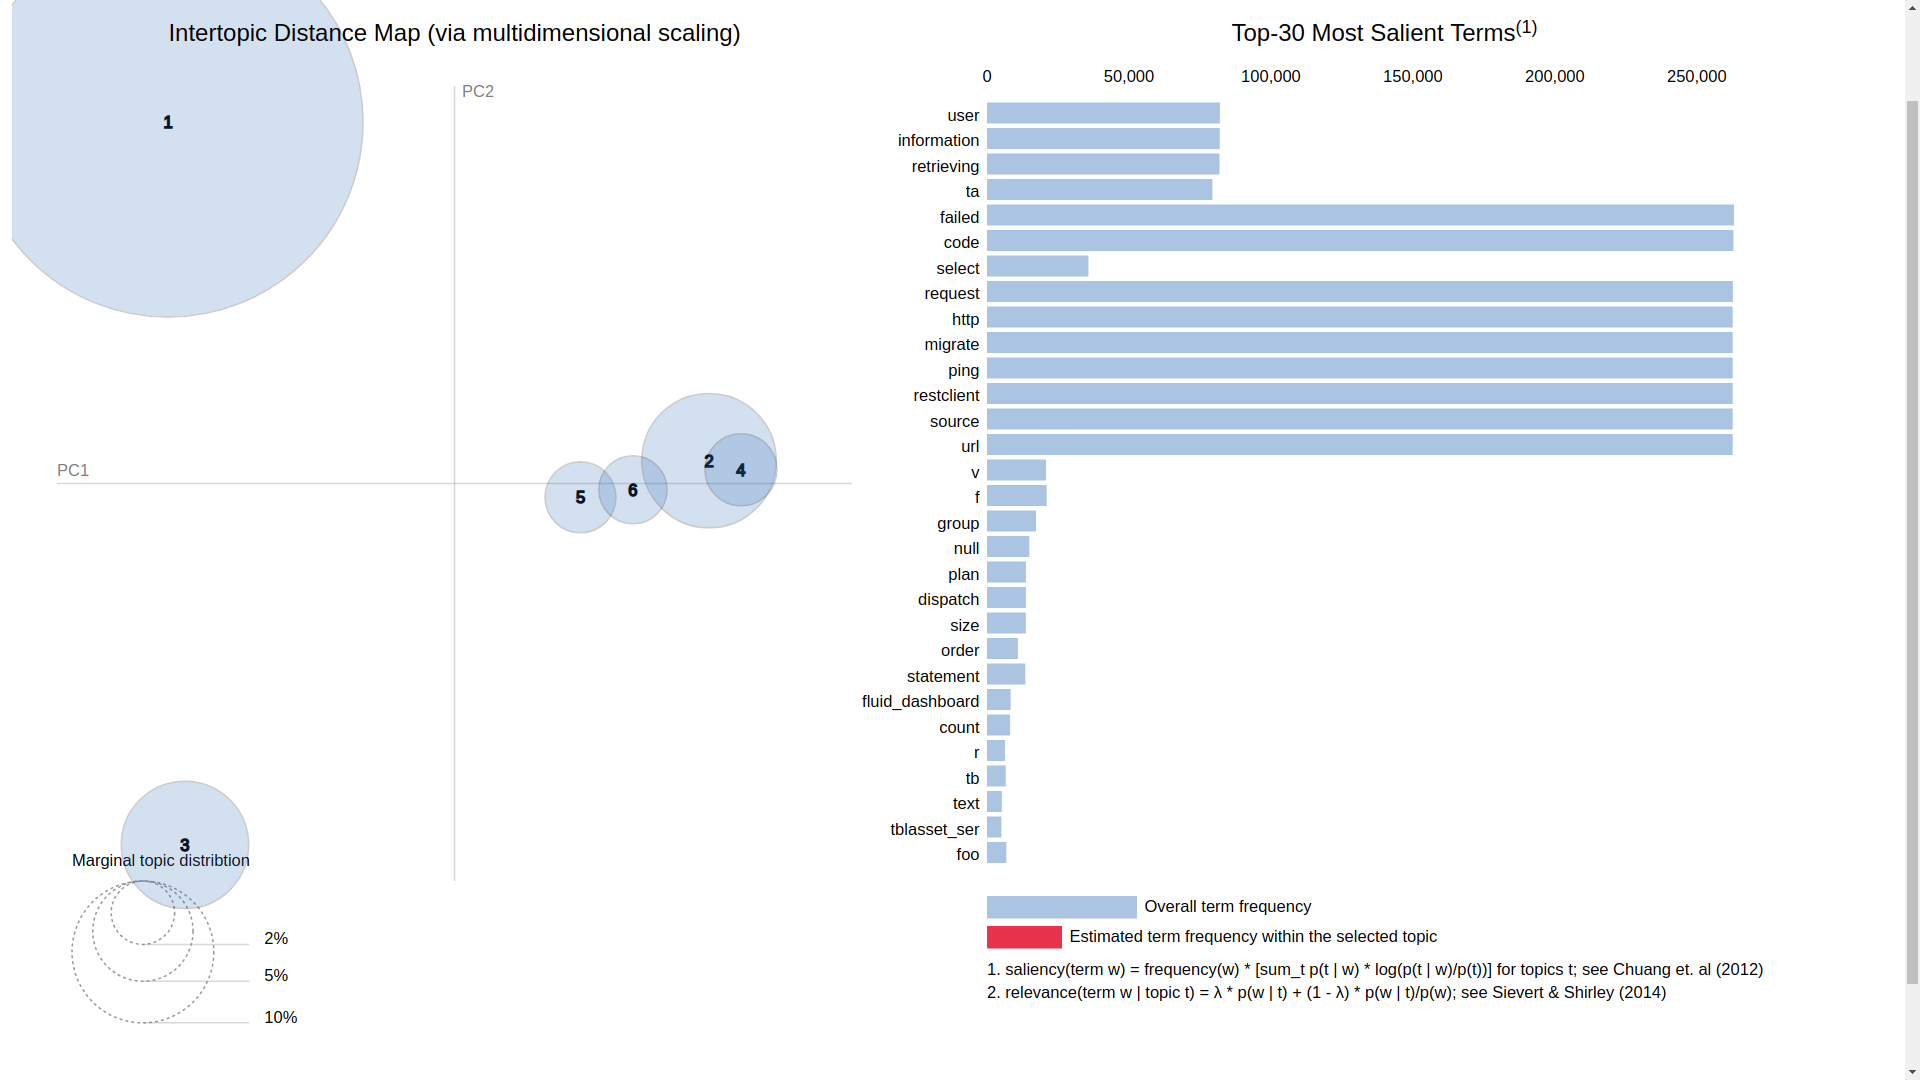
\includegraphics[width=15cm, height=8cm,trim=0 0 100px 0, clip=true]{figures/pyldavis/pyldavis_6.png}
    \caption{PyLdavis topic visualisation with 6 topics}
    \label{fig:pyldavis_6}
\end{figure}

 \begin{figure}[!h]
    \centering
    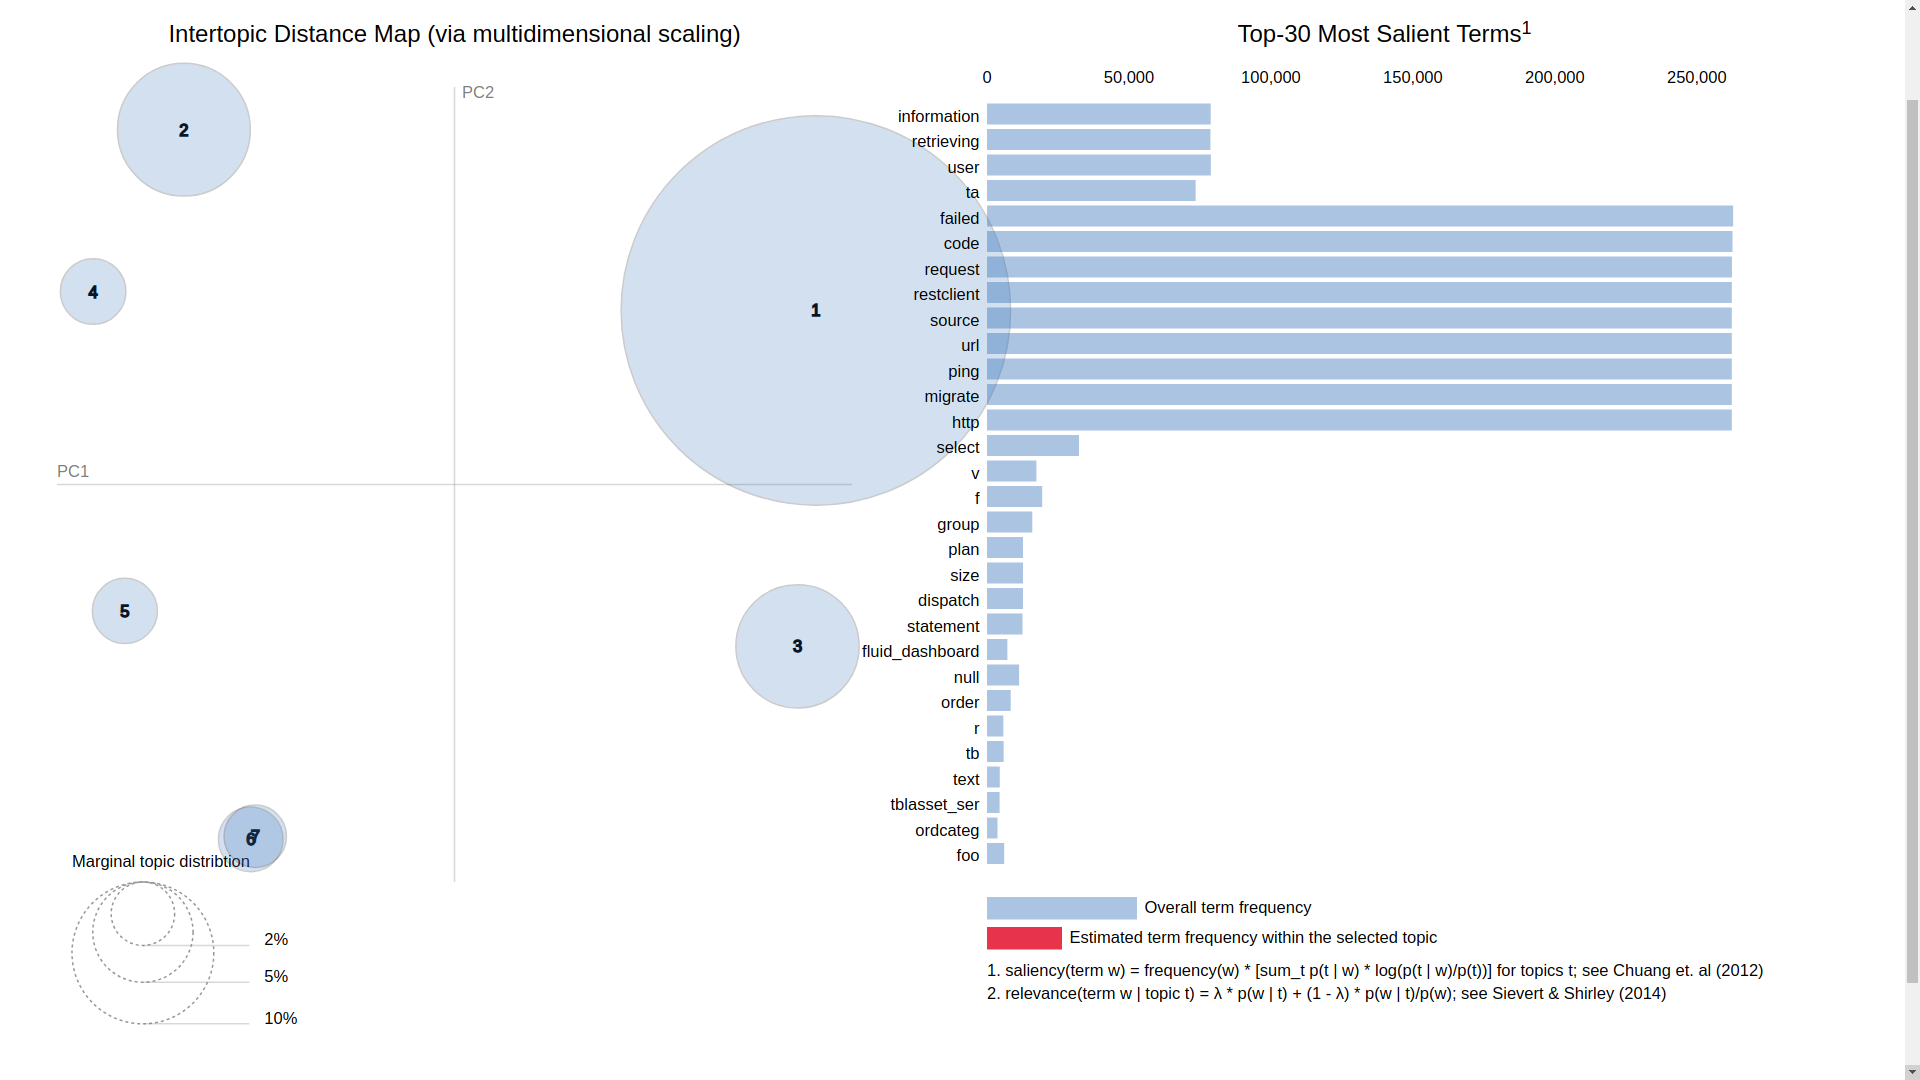
\includegraphics[width=15cm, height=8cm,trim=0 0 100px 0, clip=true]{figures/pyldavis/pyldavis_7.png}
    \caption{PyLdavis topic visualisation with 7 topics}
    \label{fig:pyldavis_7}
\end{figure}

 \begin{figure}[h]
    \centering
    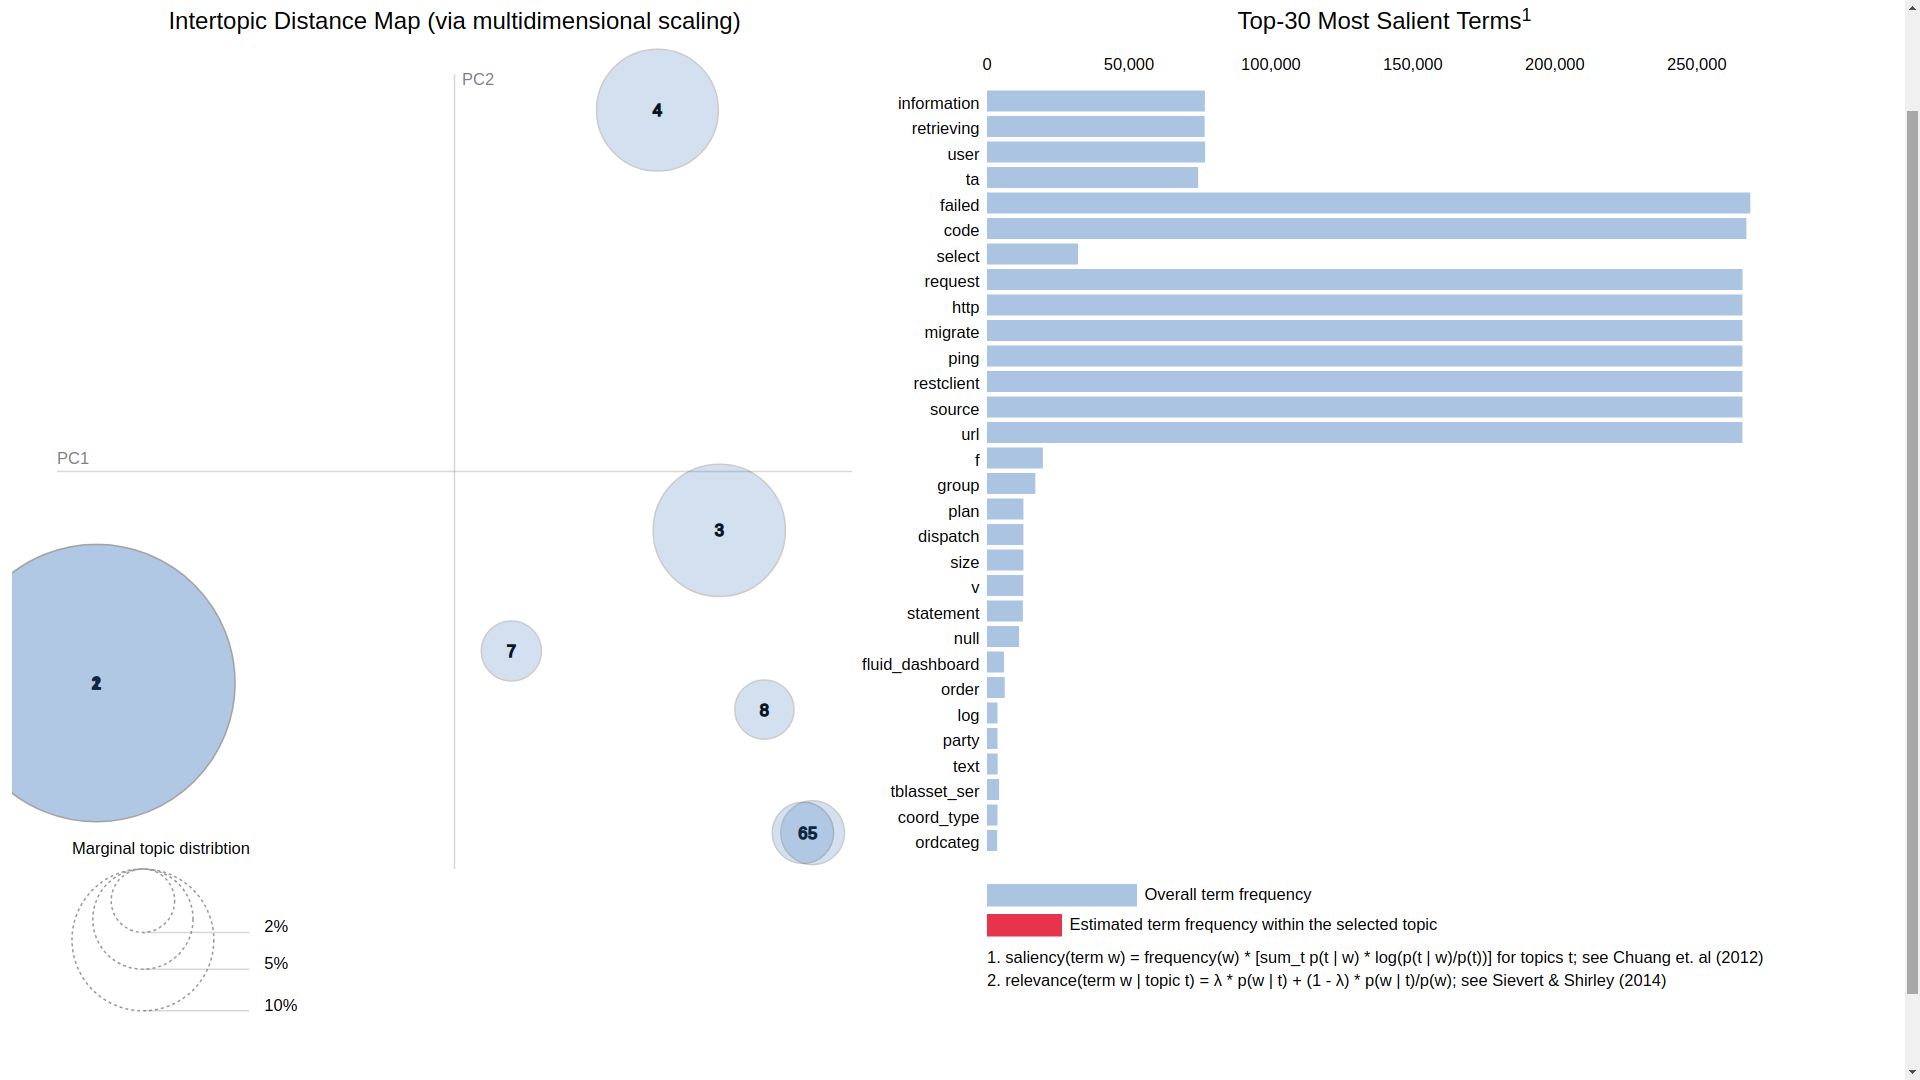
\includegraphics[width=15cm, height=8cm,trim=0 0 100px 0, clip=true]{figures/pyldavis/pyldavis_8.png}
    \caption{PyLdavis topic visualisation with 8 topics}
    \label{fig:pyldavis_8}
\end{figure}

 \begin{figure}[!h]
    \centering
    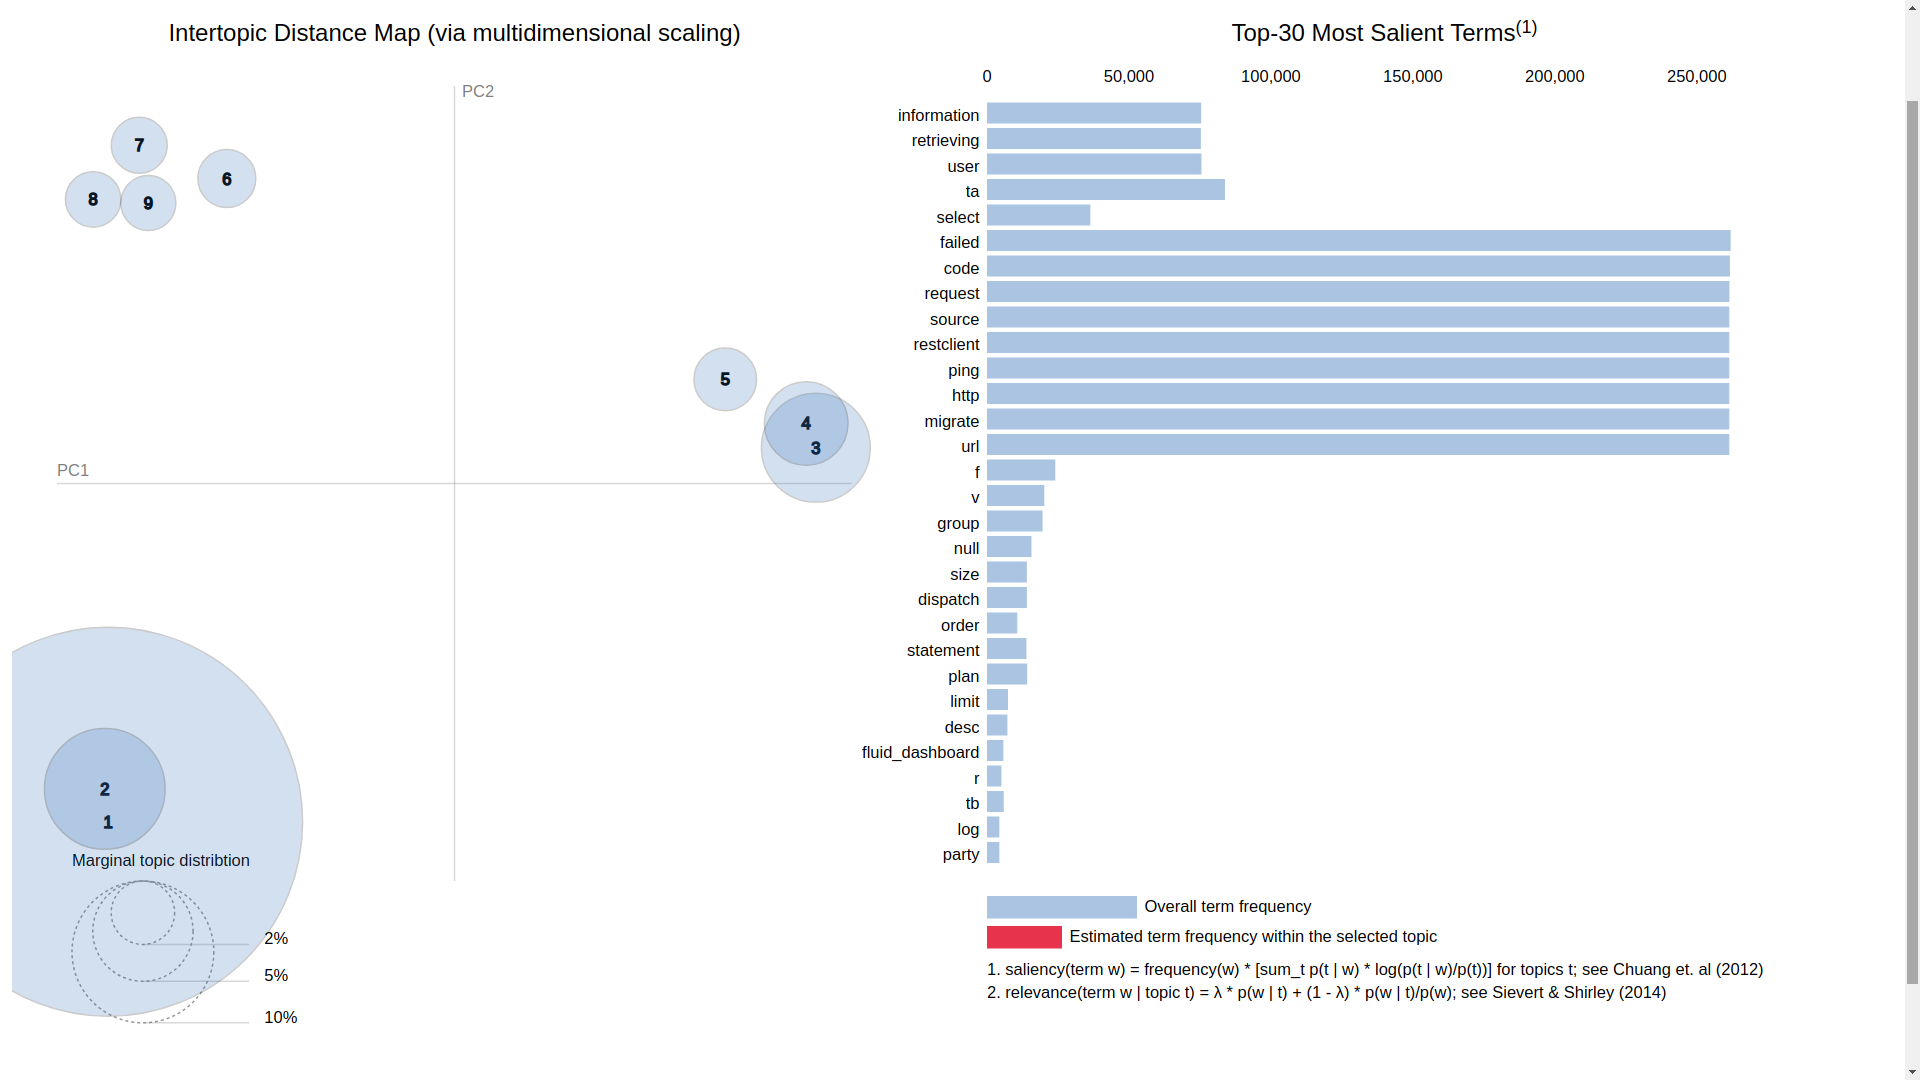
\includegraphics[width=15cm, height=8cm,trim=0 0 100px 0, clip=true]{figures/pyldavis/pyldavis_9.png}
    \caption{PyLdavis topic visualisation with 9 topics}
    \label{fig:pyldavis_9}
\end{figure}

 \begin{figure}[!h]
    \centering
    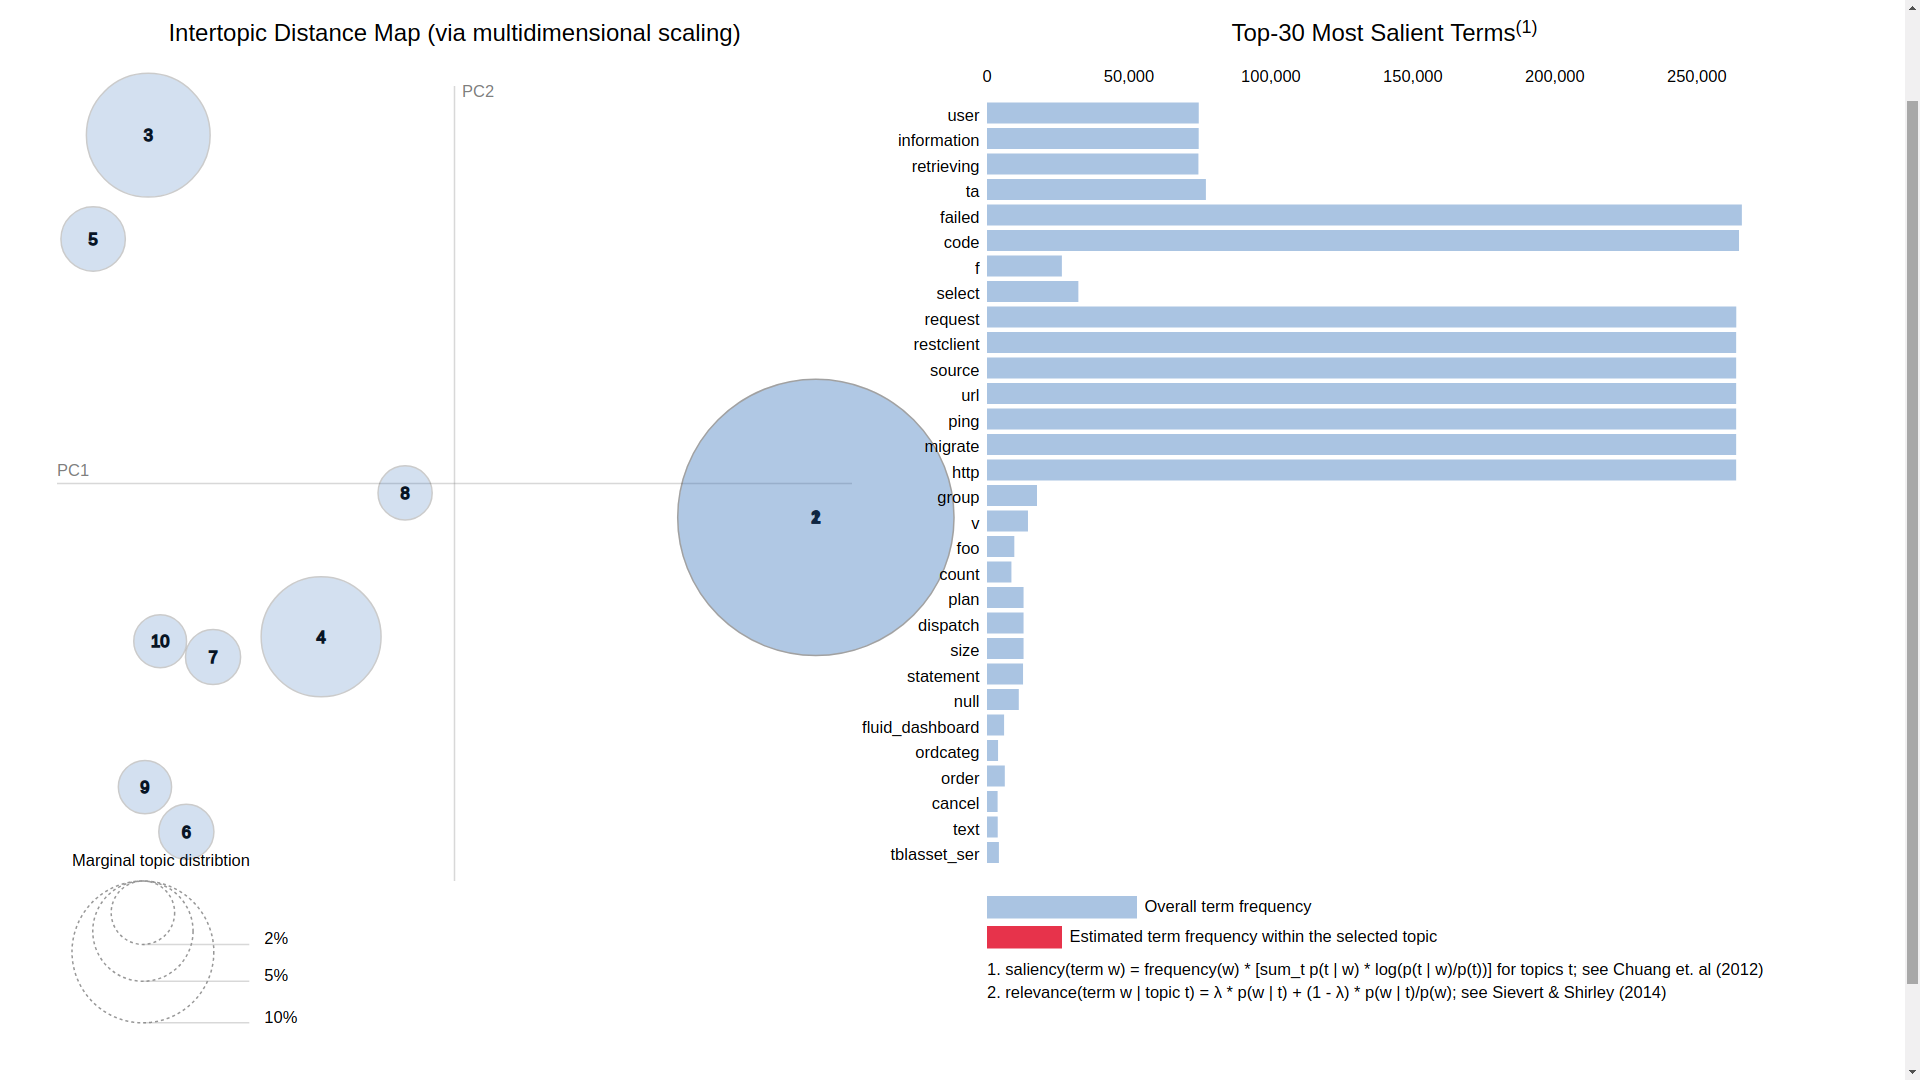
\includegraphics[width=15cm, height=8cm,trim=0 0 100px 0, clip=true]{figures/pyldavis/pyldavis_10.png}
    \caption{PyLdavis topic visualisation with 10 topics}
    \label{fig:appendices:pyldavis_10}
\end{figure}

 \begin{figure}[!h]
    \centering
    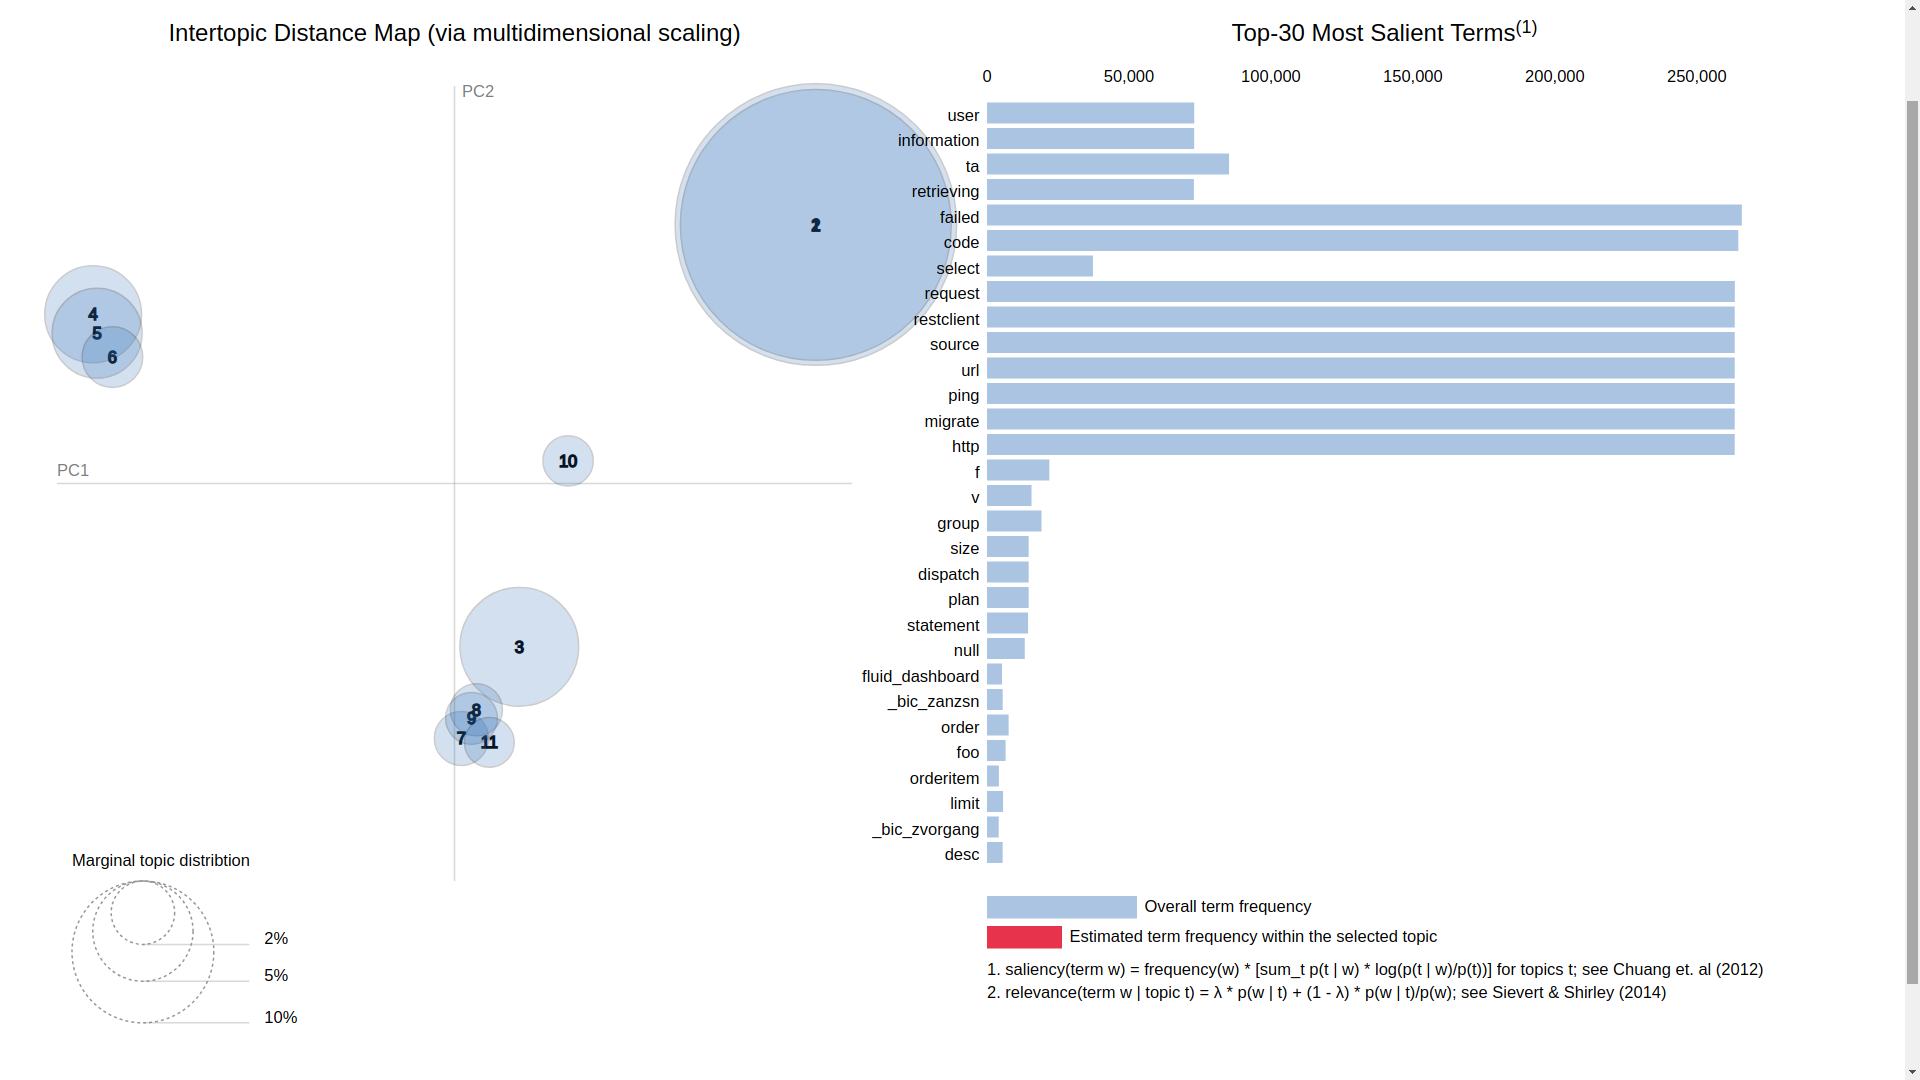
\includegraphics[width=15cm, height=8cm,trim=0 0 100px 0, clip=true]{figures/pyldavis/pyldavis_11.png}
    \caption{PyLdavis topic visualisation with 11 topics}
    \label{fig:pyldavis_11}
\end{figure}

 \begin{figure}[!h]
    \centering
    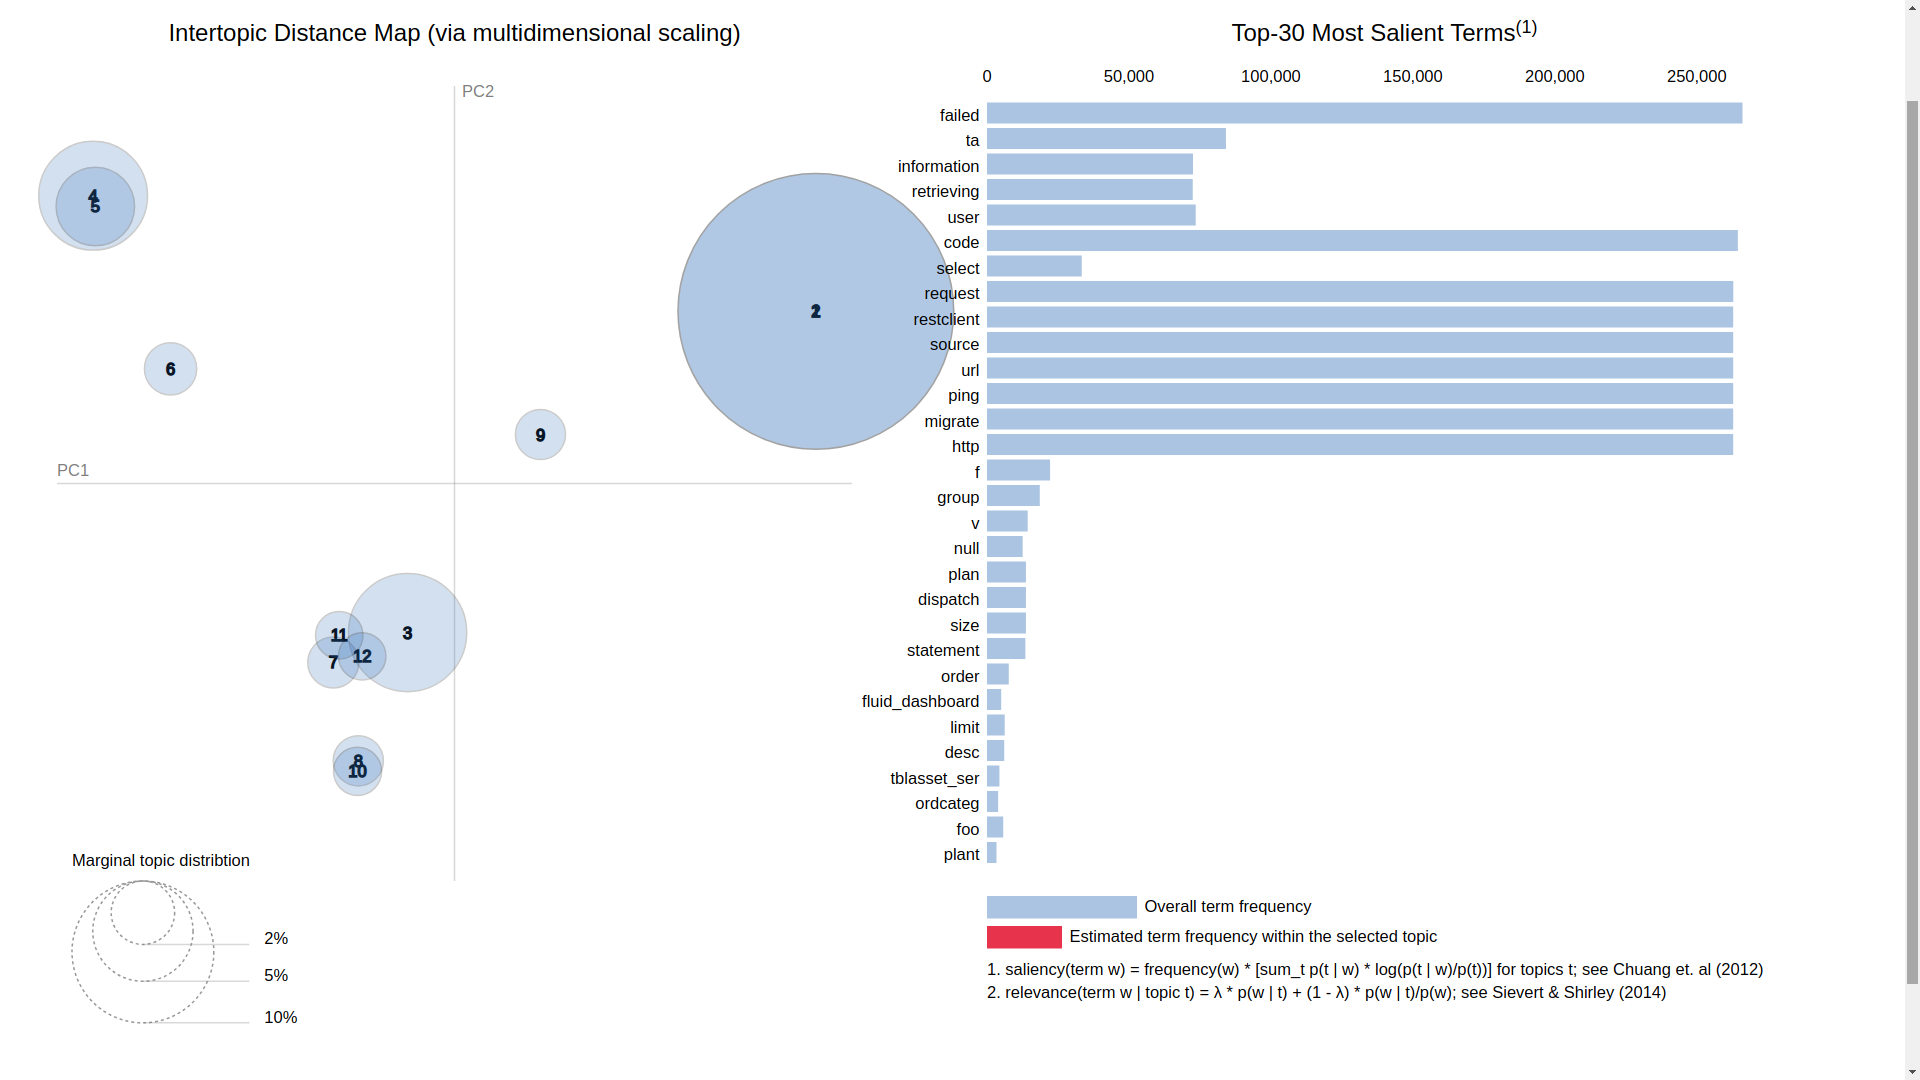
\includegraphics[width=15cm, height=8cm,trim=0 0 100px 0, clip=true]{figures/pyldavis/pyldavis_12.png}
    \caption{PyLdavis topic visualisation with 12 topics}
    \label{fig:pyldavis_12}
\end{figure}

 \begin{figure}[!h]
    \centering
    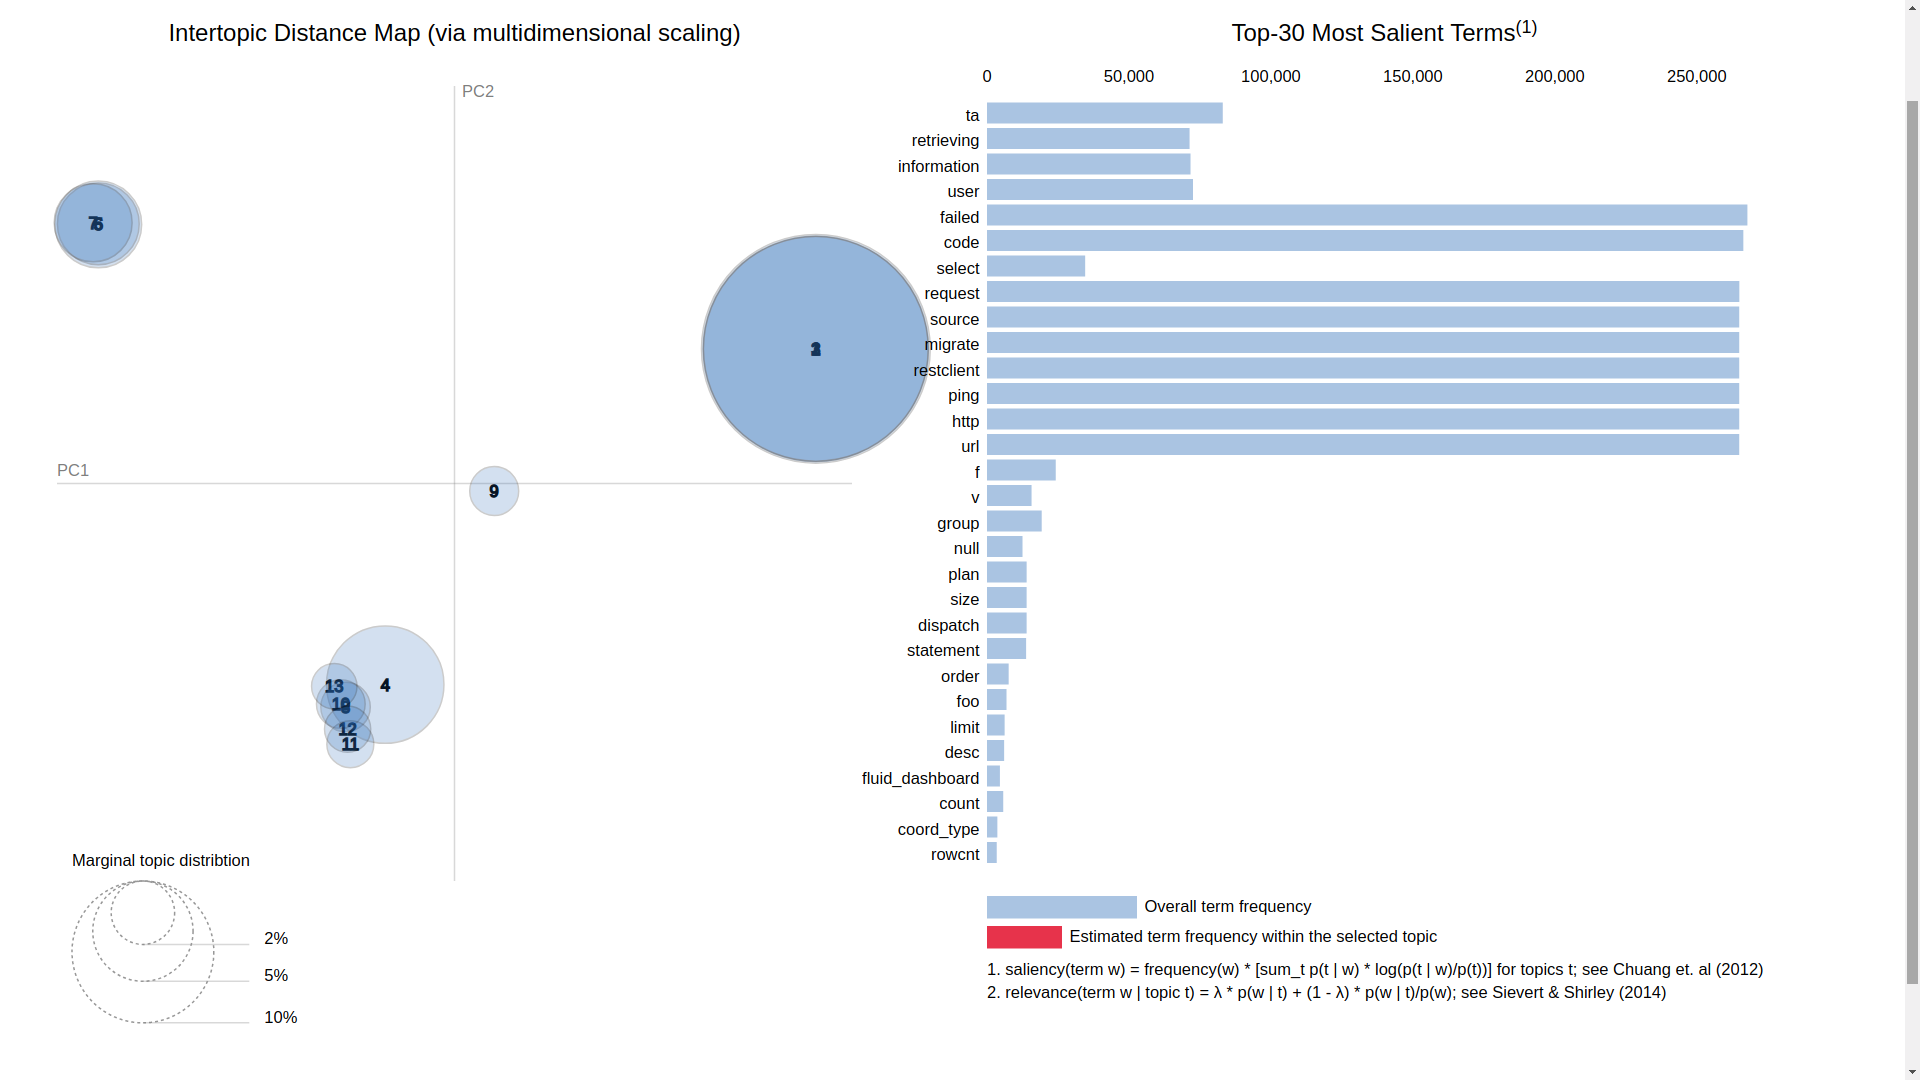
\includegraphics[width=15cm, height=8cm,trim=0 0 100px 0, clip=true]{figures/pyldavis/pyldavis_13.png}
    \caption{PyLdavis topic visualisation with 13 topics}
    \label{fig:pyldavis_13}
\end{figure}

 \begin{figure}[!h]
    \centering
    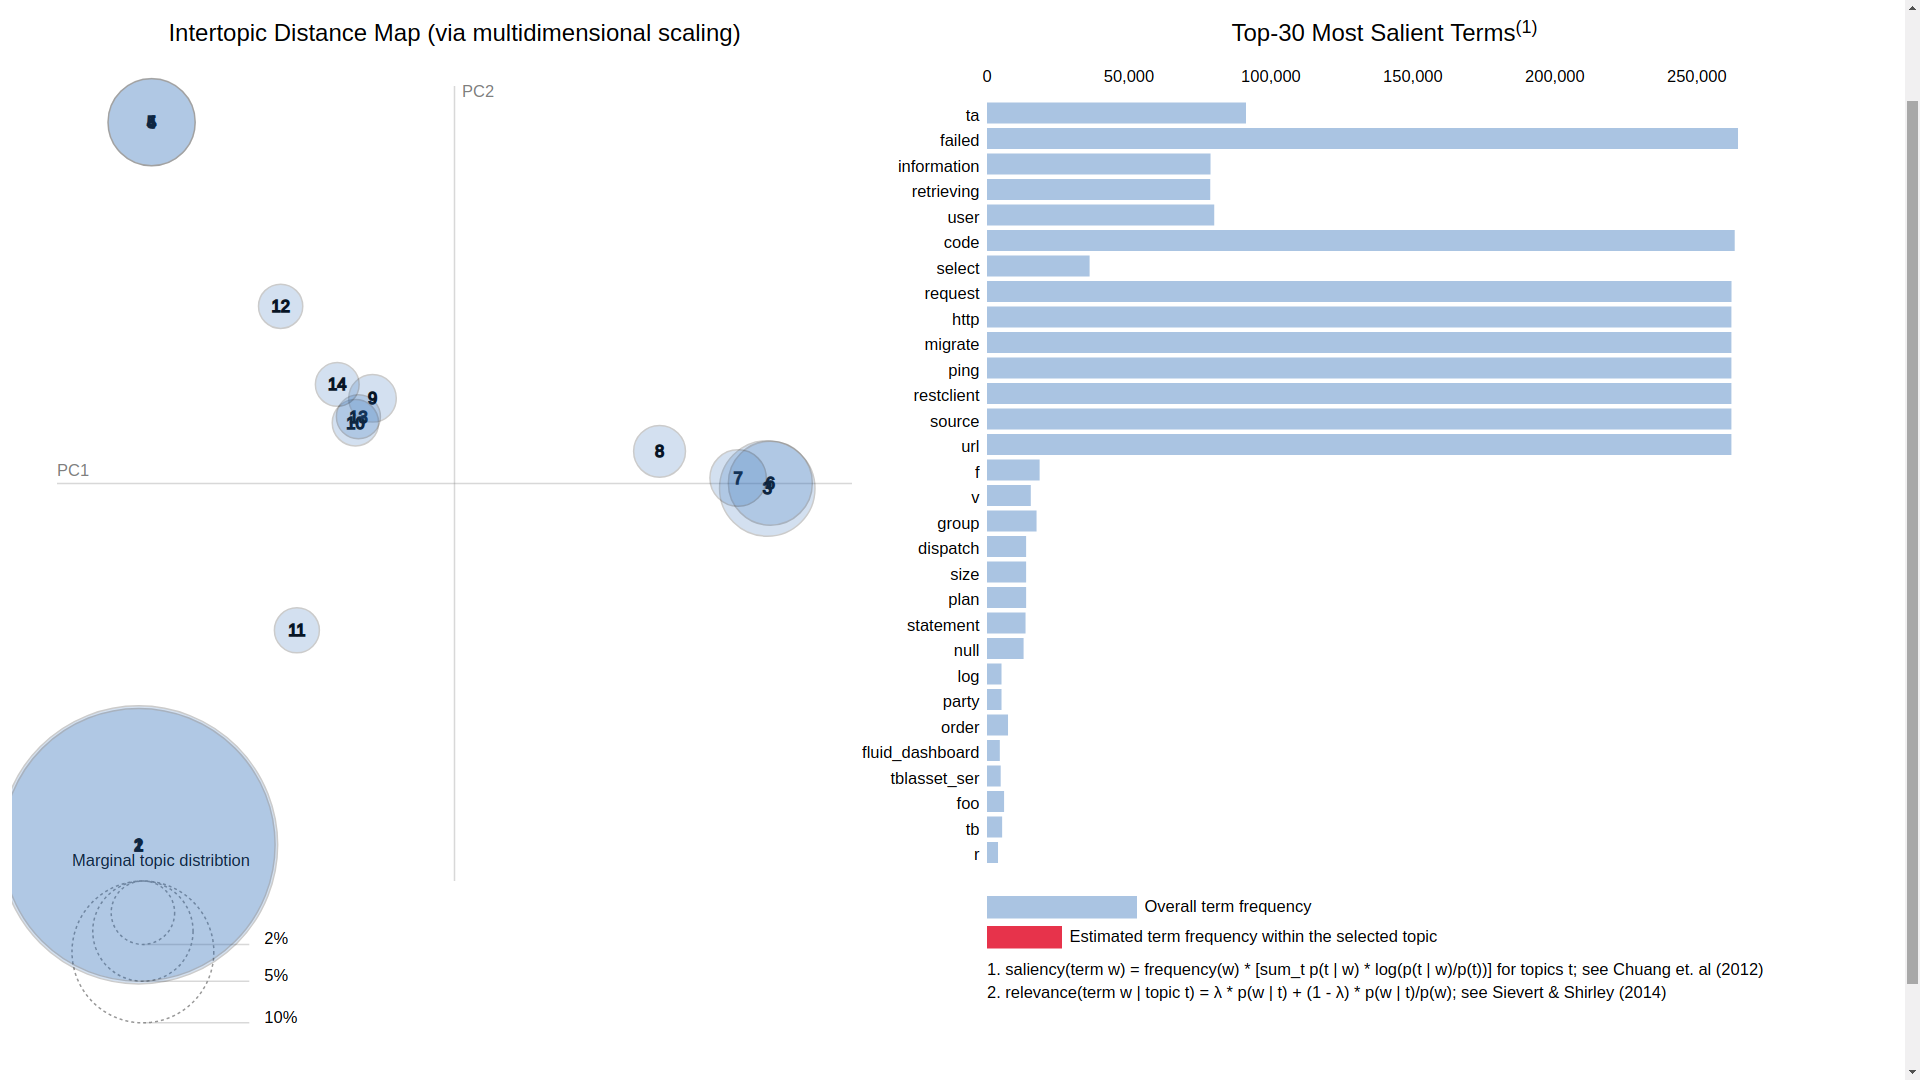
\includegraphics[width=15cm, height=8cm,trim=0 0 100px 0, clip=true]{figures/pyldavis/pyldavis_14.png}
    \caption{PyLdavis topic visualisation with 14 topics}
    \label{fig:pyldavis_14}
\end{figure}

 \begin{figure}[!h]
    \centering
    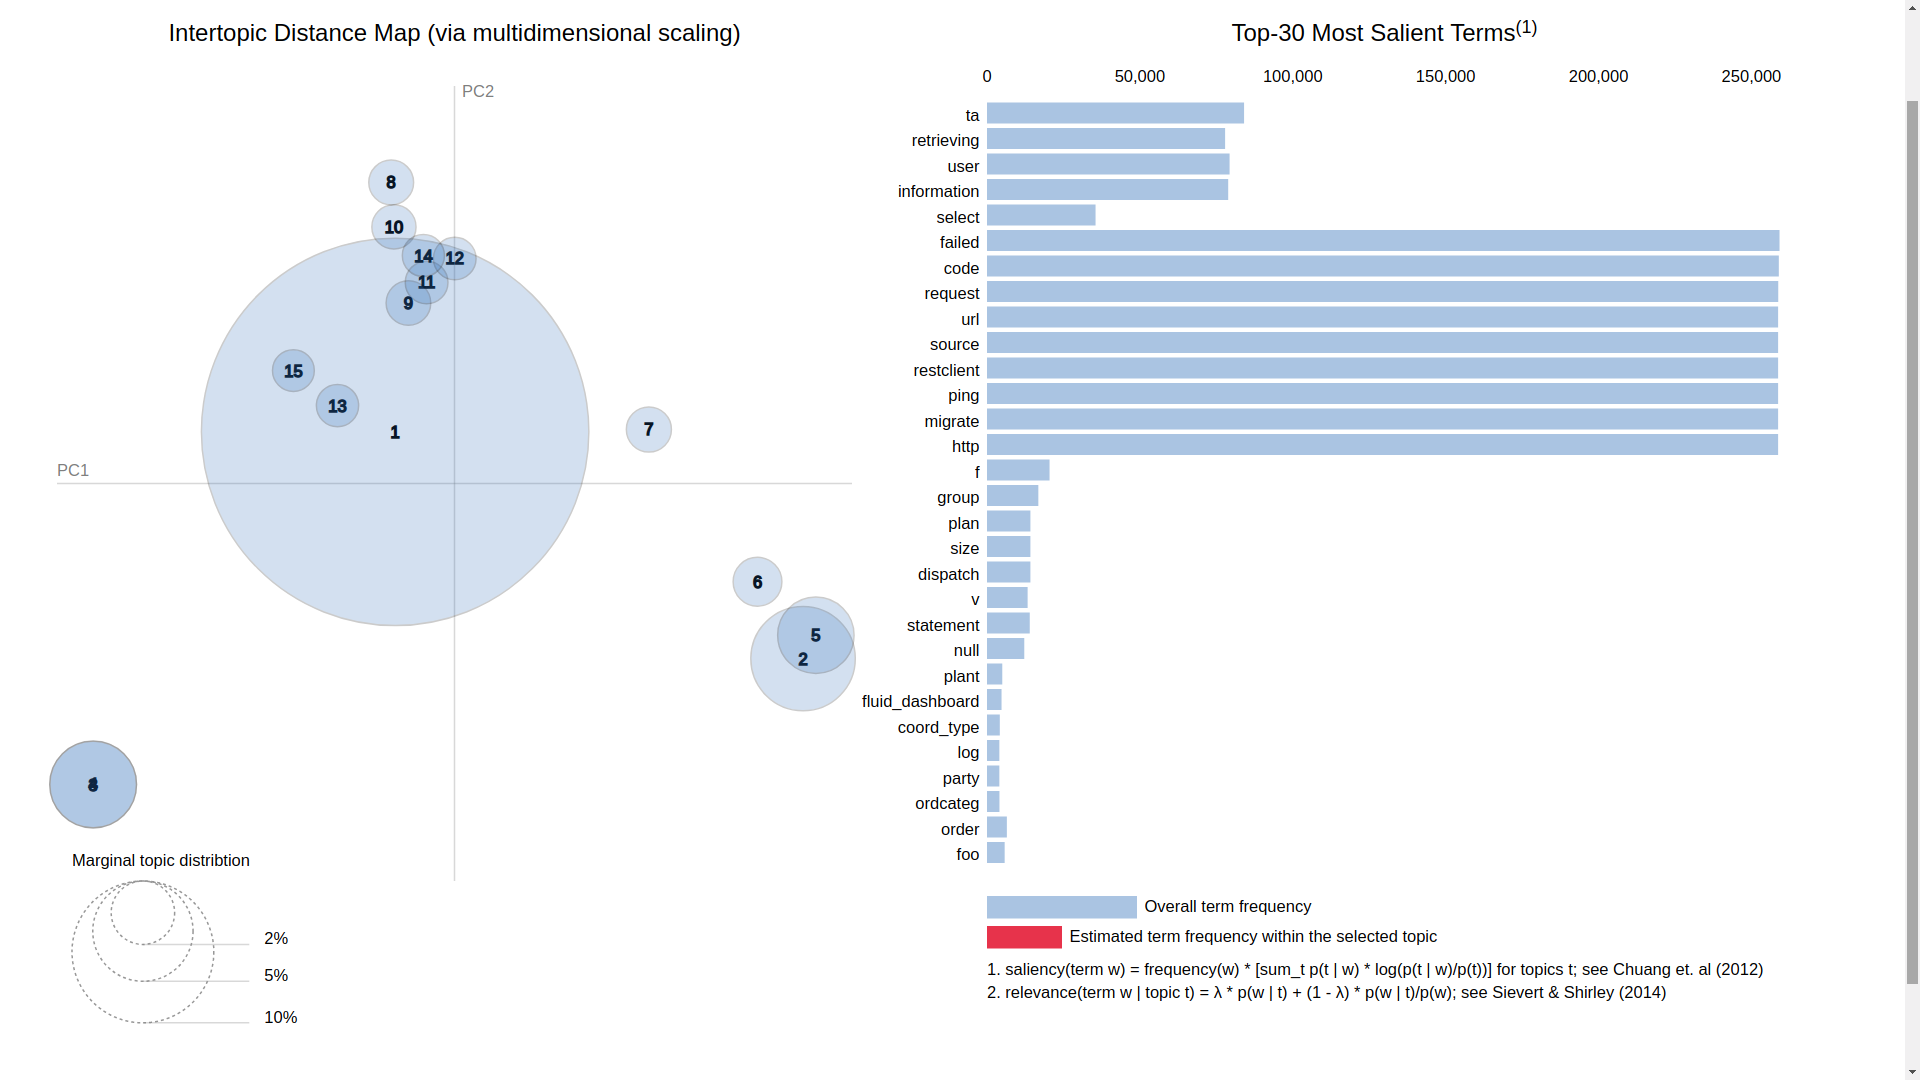
\includegraphics[width=15cm, height=8cm,trim=0 0 100px 0, clip=true]{figures/pyldavis/pyldavis_15.png}
    \caption{PyLdavis topic visualisation with 15 topics}
    \label{fig:pyldavis_15}
\end{figure}

 \begin{figure}[!h]
    \centering
    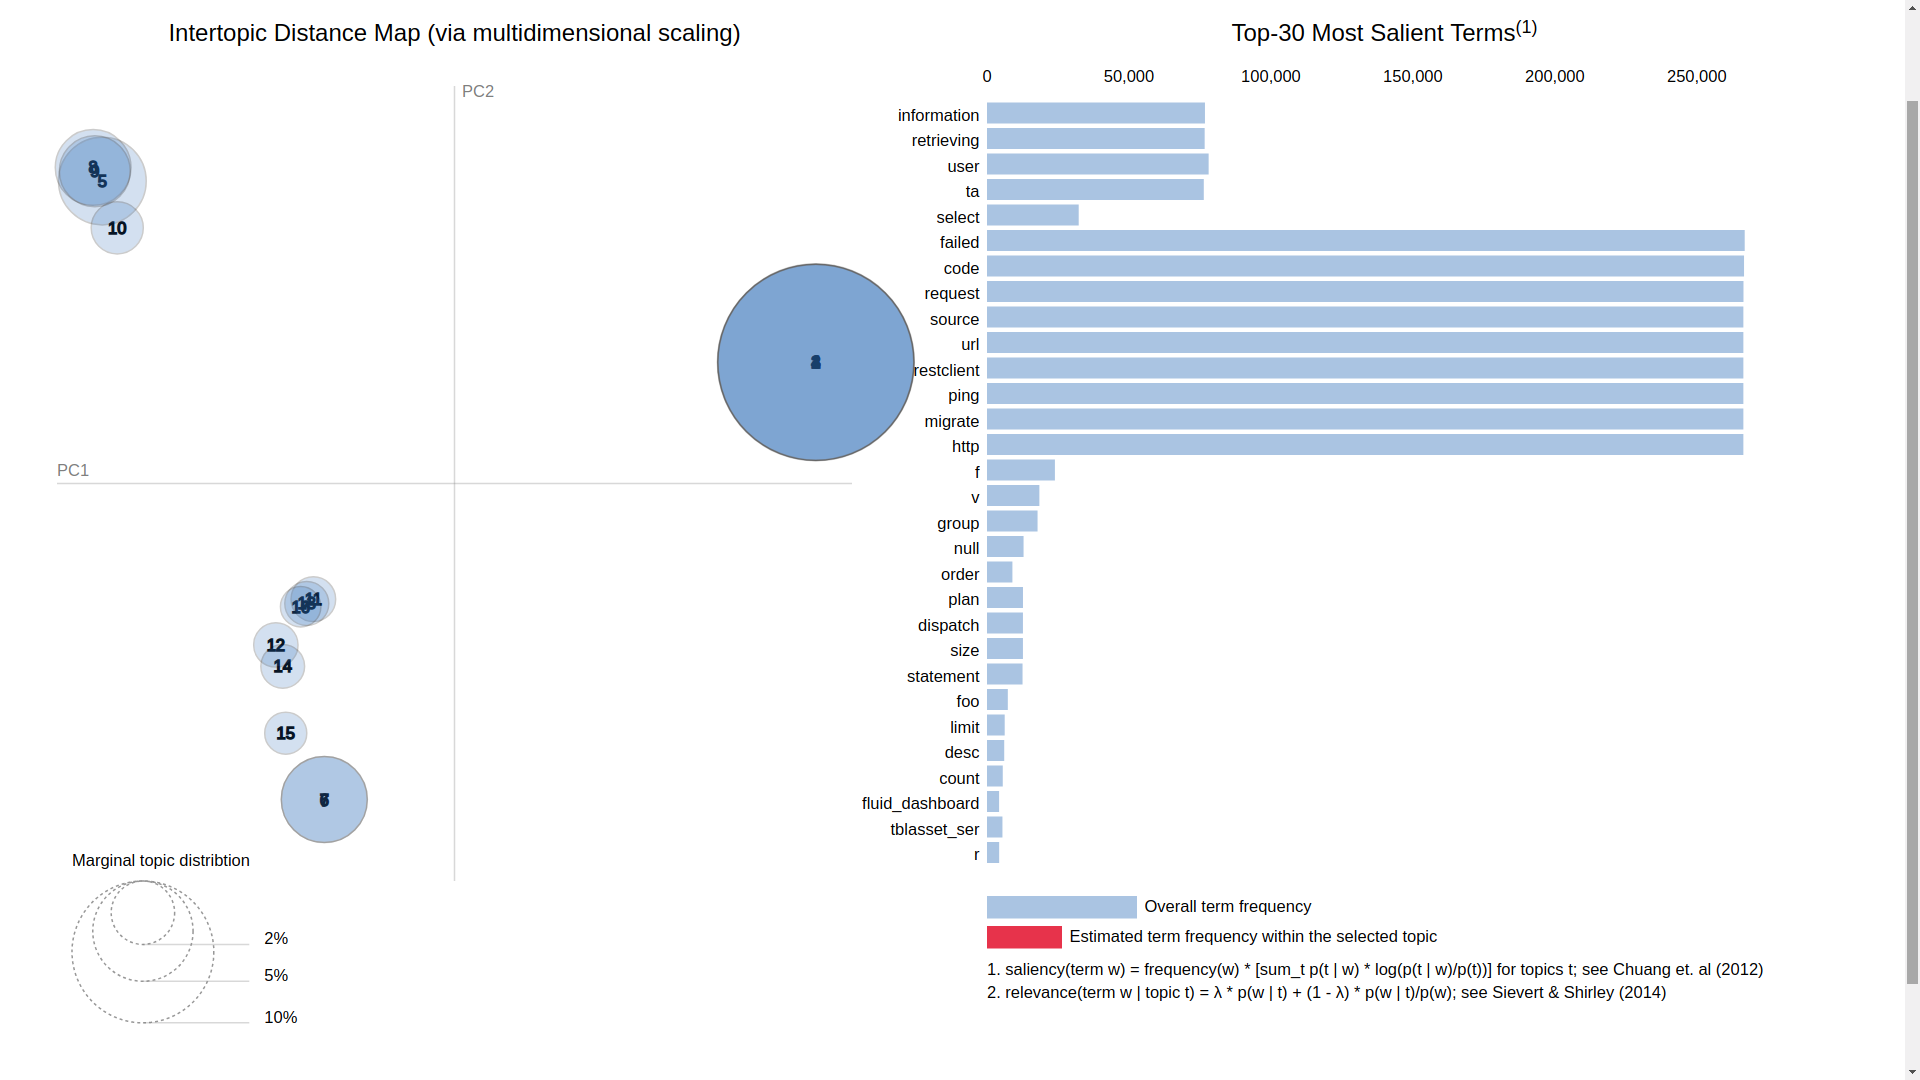
\includegraphics[width=15cm, height=8cm,trim=0 0 100px 0, clip=true]{figures/pyldavis/pyldavis_16.png}
    \caption{PyLdavis topic visualisation with 16 topics}
    \label{fig:pyldavis_16}
\end{figure}

 \begin{figure}[!h]
    \centering
    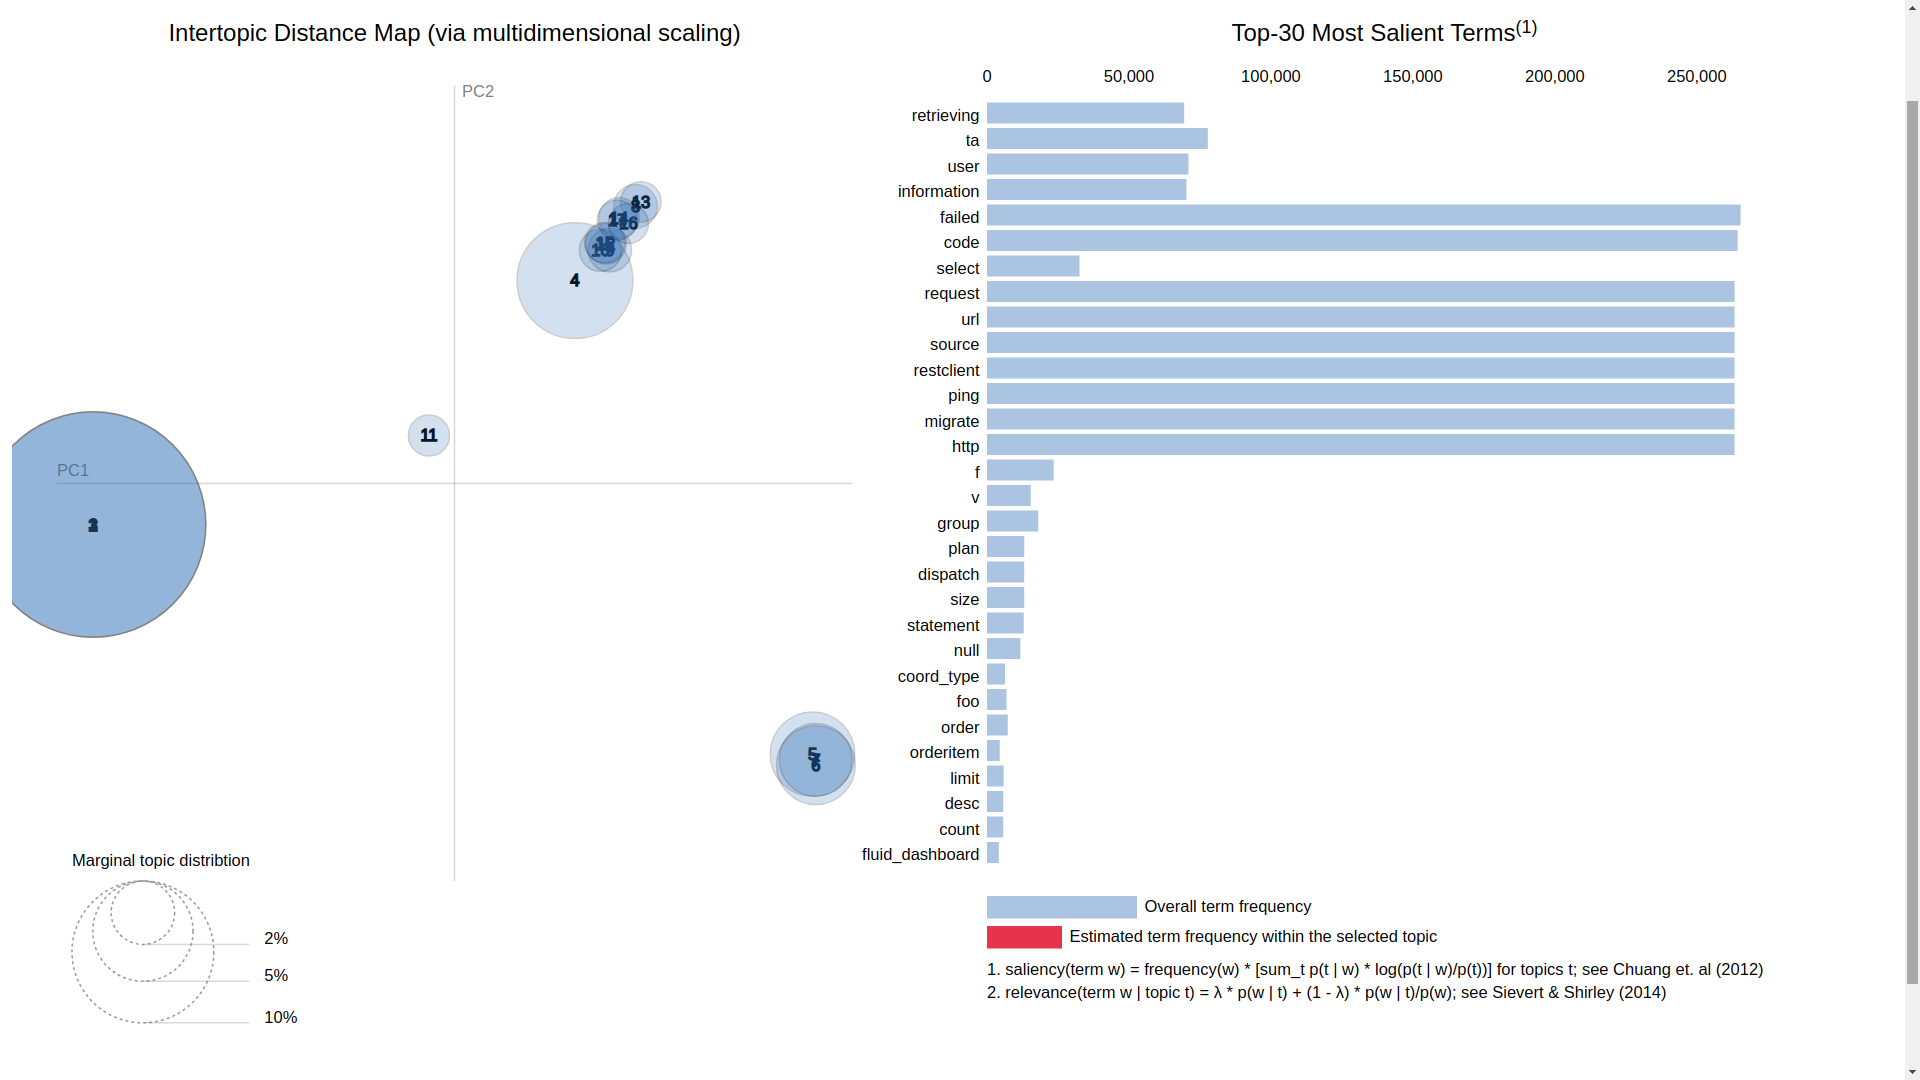
\includegraphics[width=15cm, height=8cm,trim=0 0 100px 0, clip=true]{figures/pyldavis/pyldavis_17.png}
    \caption{PyLdavis topic visualisation with 17 topics}
    \label{fig:pyldavis_17}
\end{figure}

 \begin{figure}[!h]
    \centering
    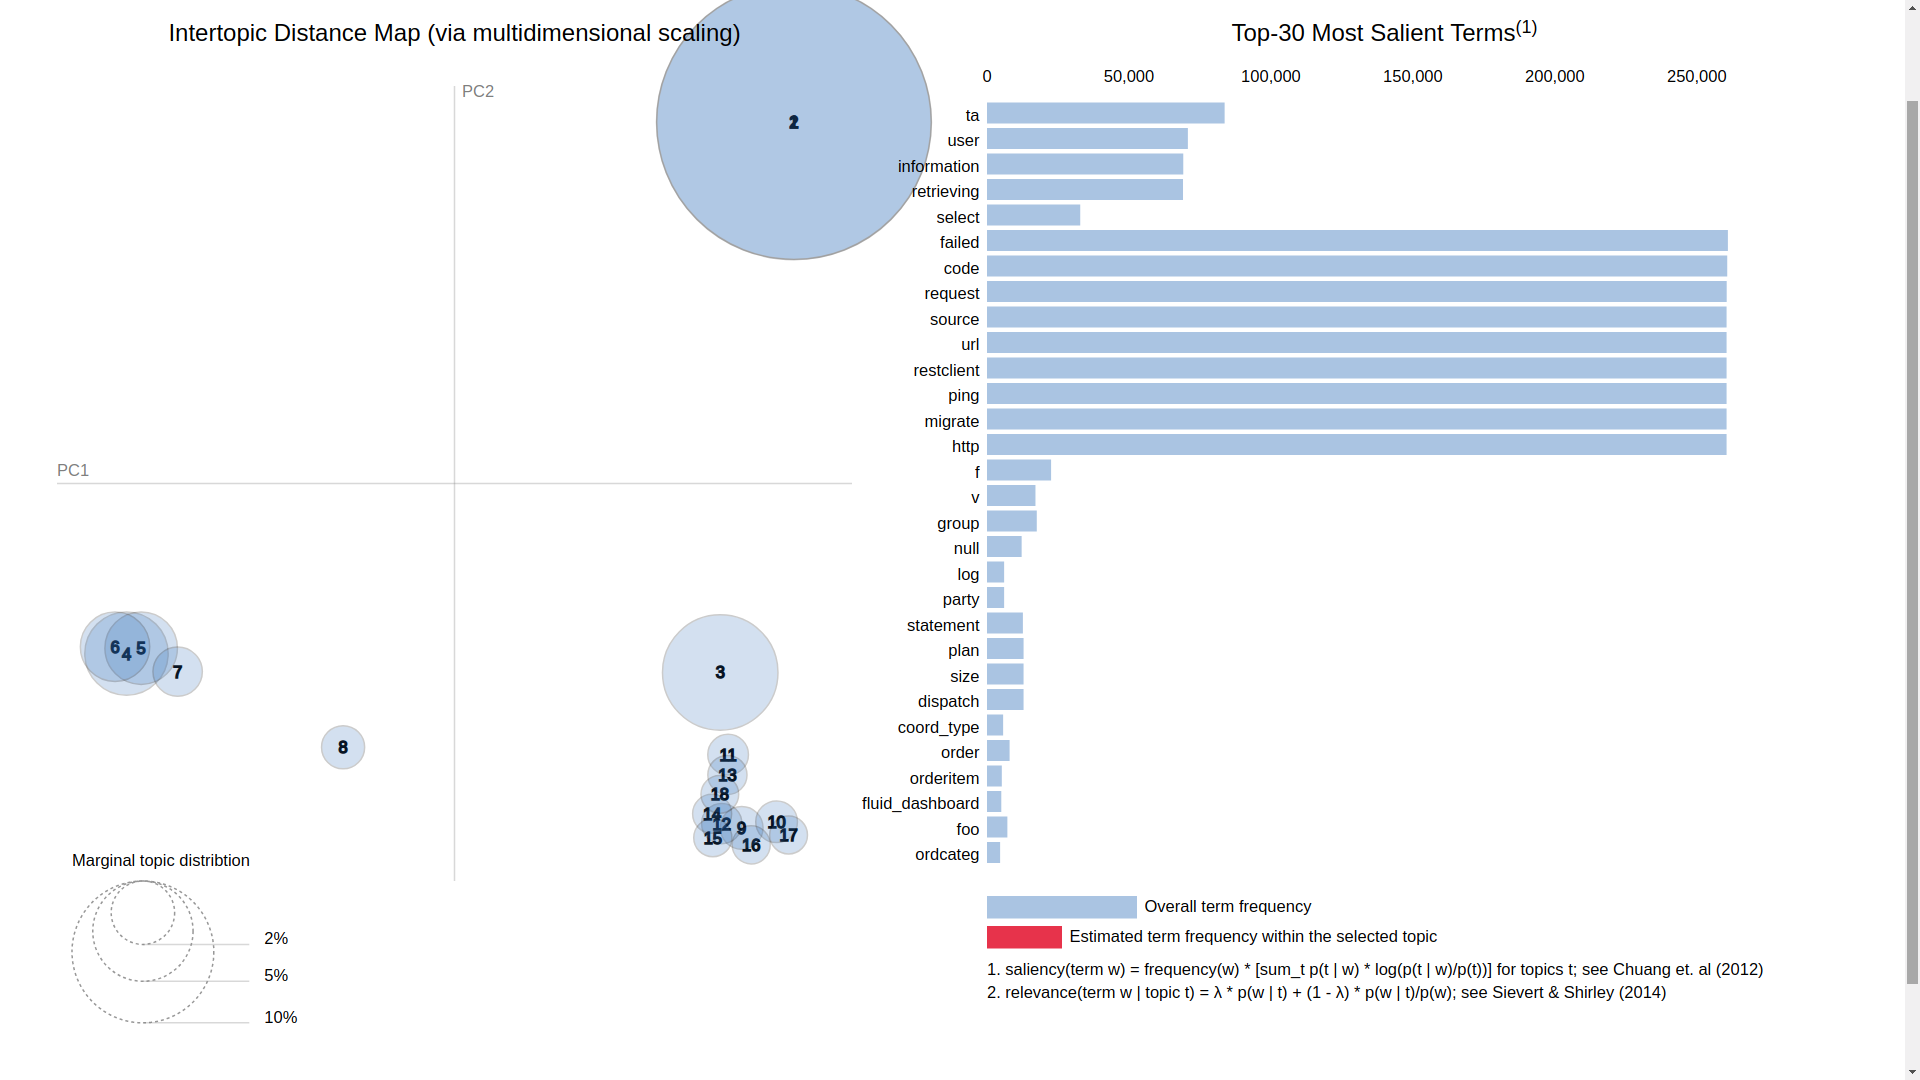
\includegraphics[width=15cm, height=8cm,trim=0 0 100px 0, clip=true]{figures/pyldavis/pyldavis_18.png}
    \caption{PyLdavis topic visualisation with 18 topics}
    \label{fig:pyldavis_18}
\end{figure}

 \begin{figure}[!h]
    \centering
    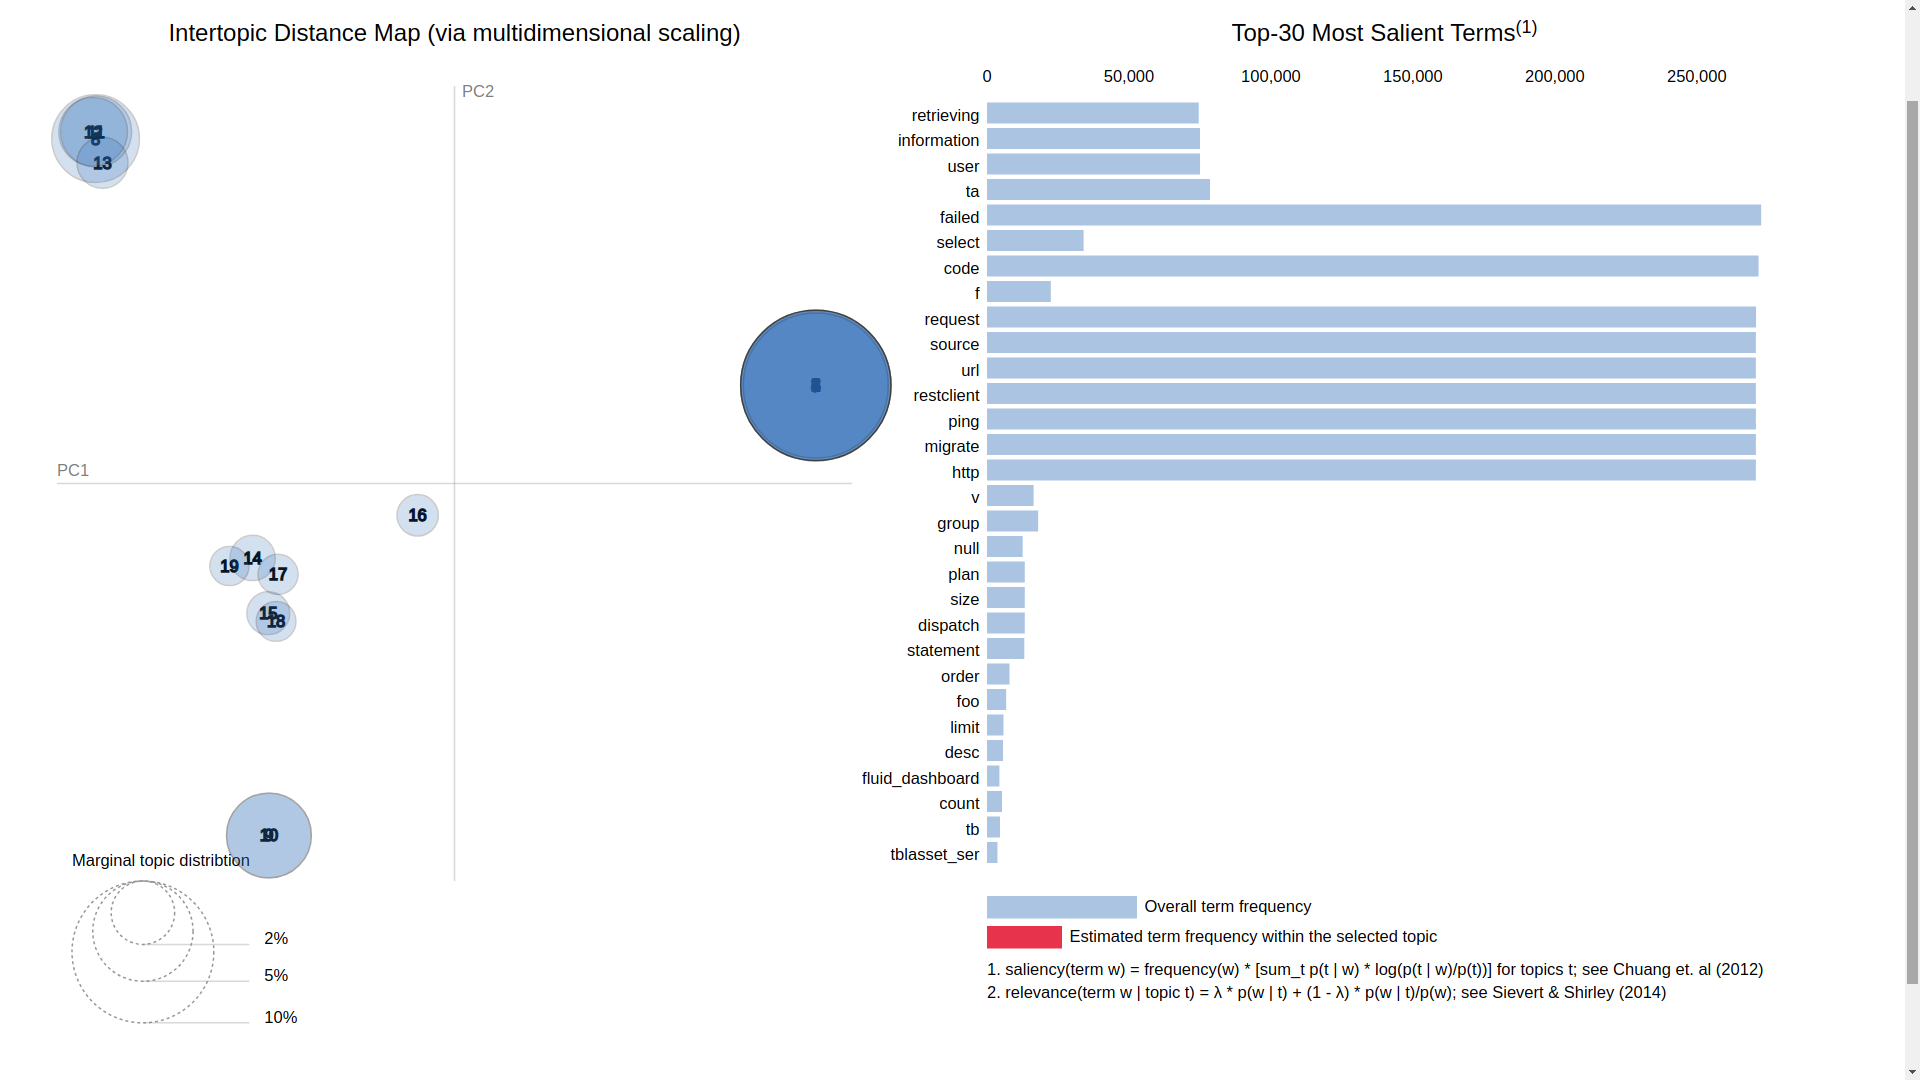
\includegraphics[width=15cm, height=8cm,trim=0 0 100px 0, clip=true]{figures/pyldavis/pyldavis_19.png}
    \caption{PyLdavis topic visualisation with 19 topics}
    \label{fig:pyldavis_19}
\end{figure}

 \begin{figure}[!h]
    \centering
    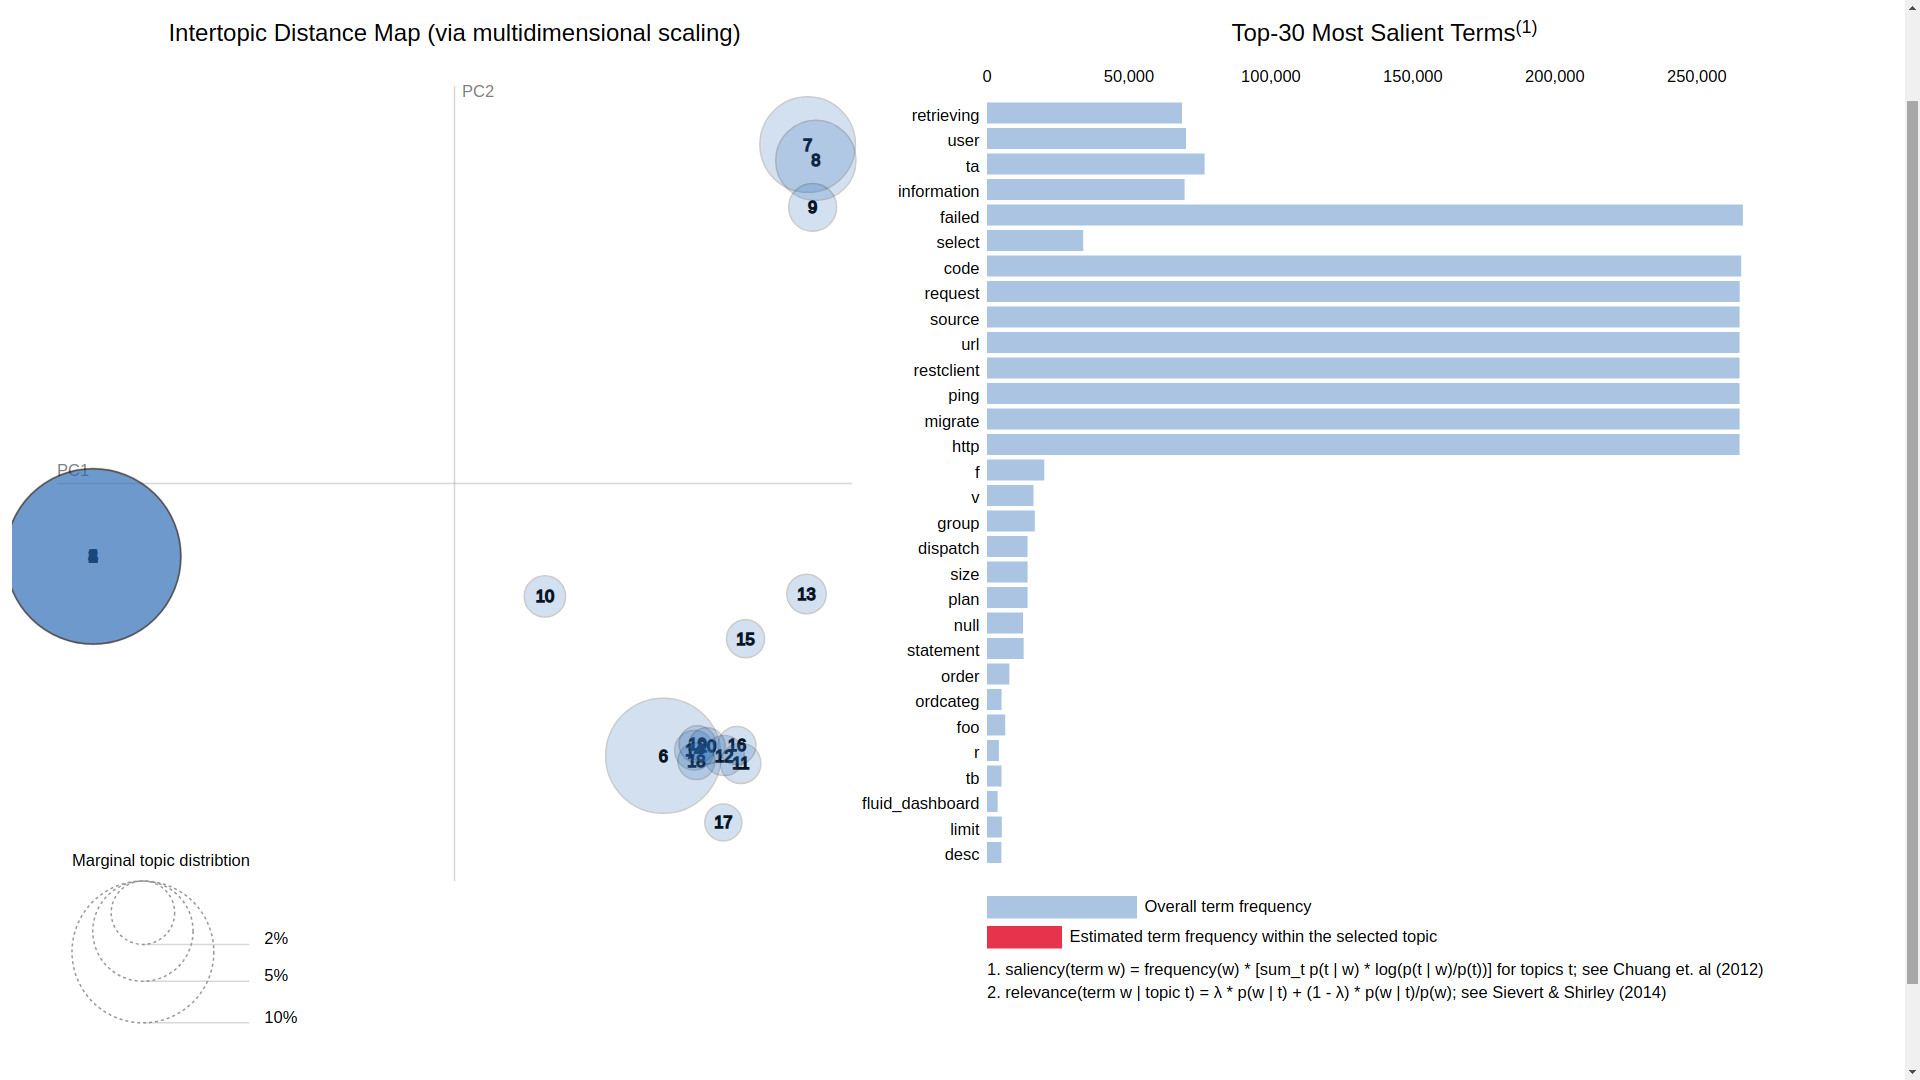
\includegraphics[width=15cm, height=8cm,trim=0 0 100px 0, clip=true]{figures/pyldavis/pyldavis_20.png}
    \caption{PyLdavis topic visualisation with 20 topics}
    \label{fig:pyldavis_20}
\end{figure}

 \begin{figure}[!h]
    \centering
    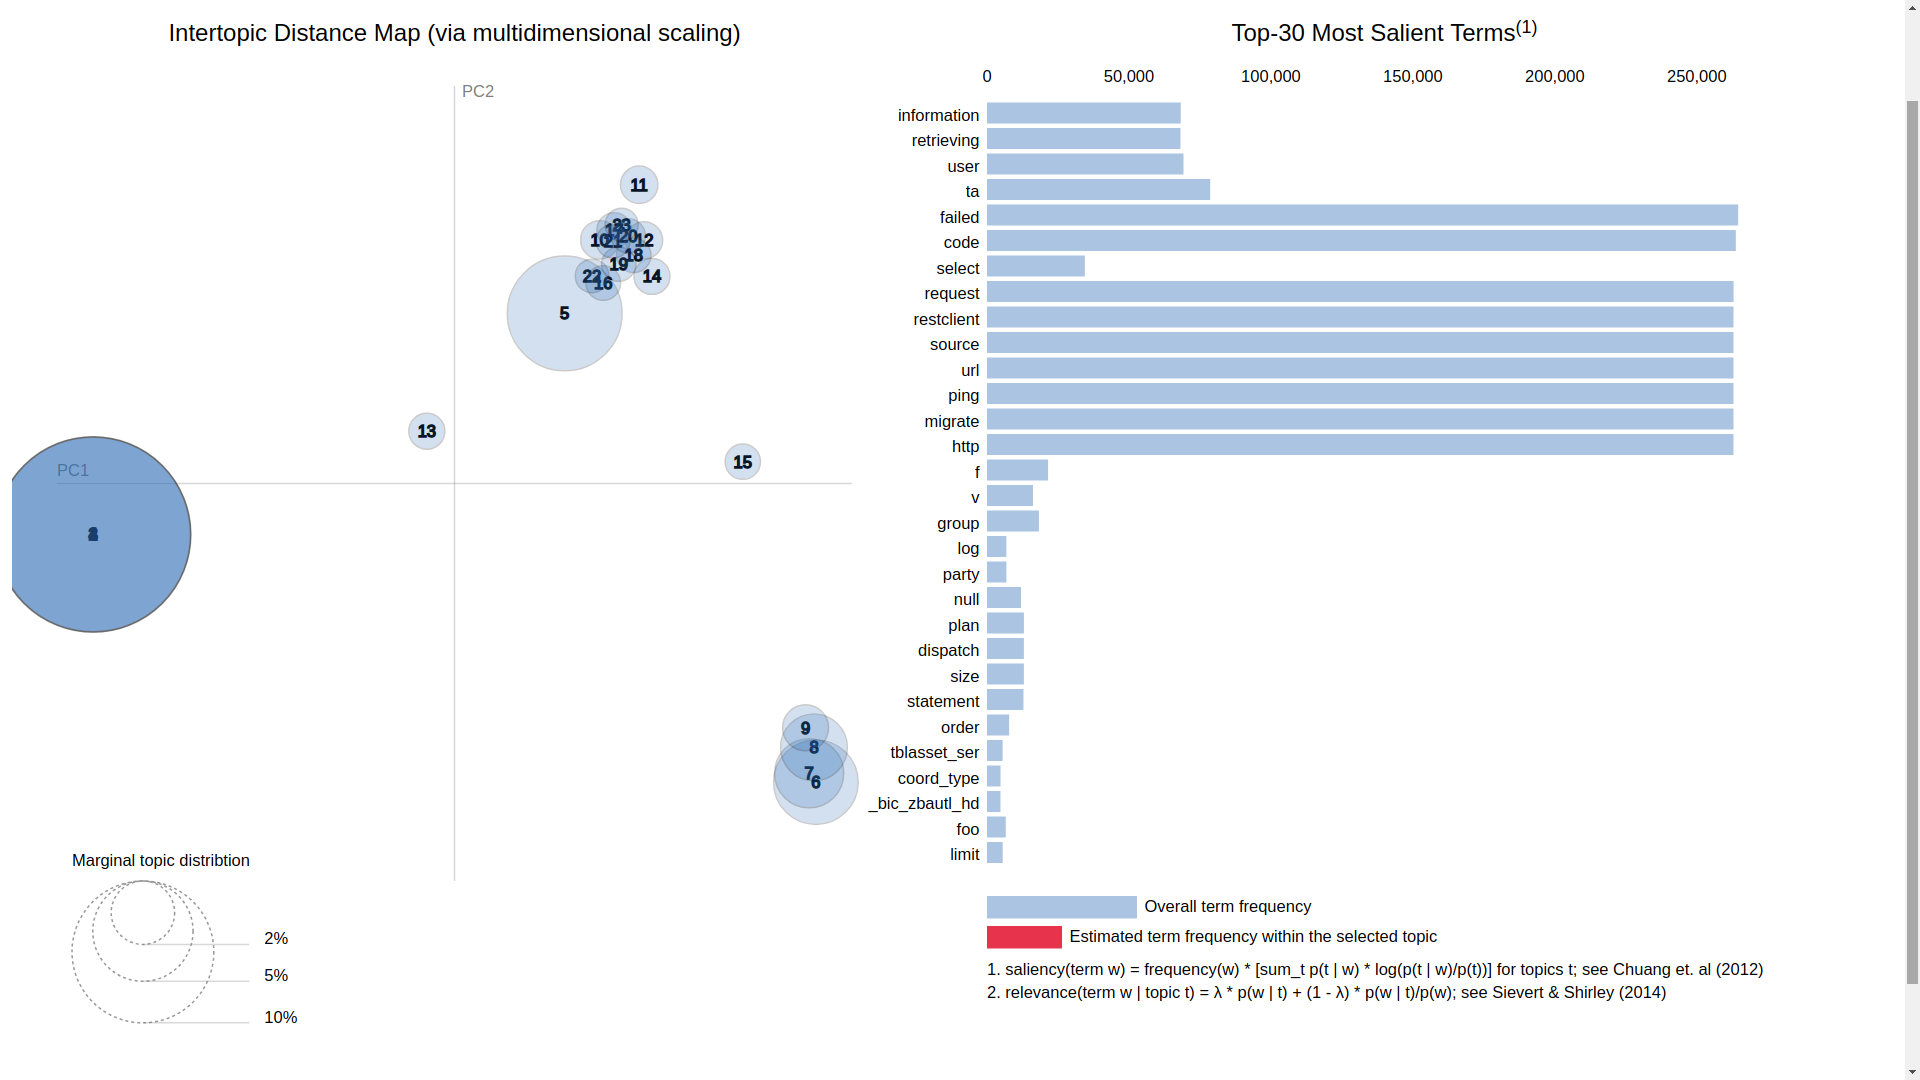
\includegraphics[width=15cm, height=8cm,trim=0 0 100px 0, clip=true]{figures/pyldavis/pyldavis_23.png}
    \caption{PyLdavis topic visualisation with 23 topics}
    \label{fig:pyldavis_23}
\end{figure}

 \begin{figure}[!h]
    \centering
    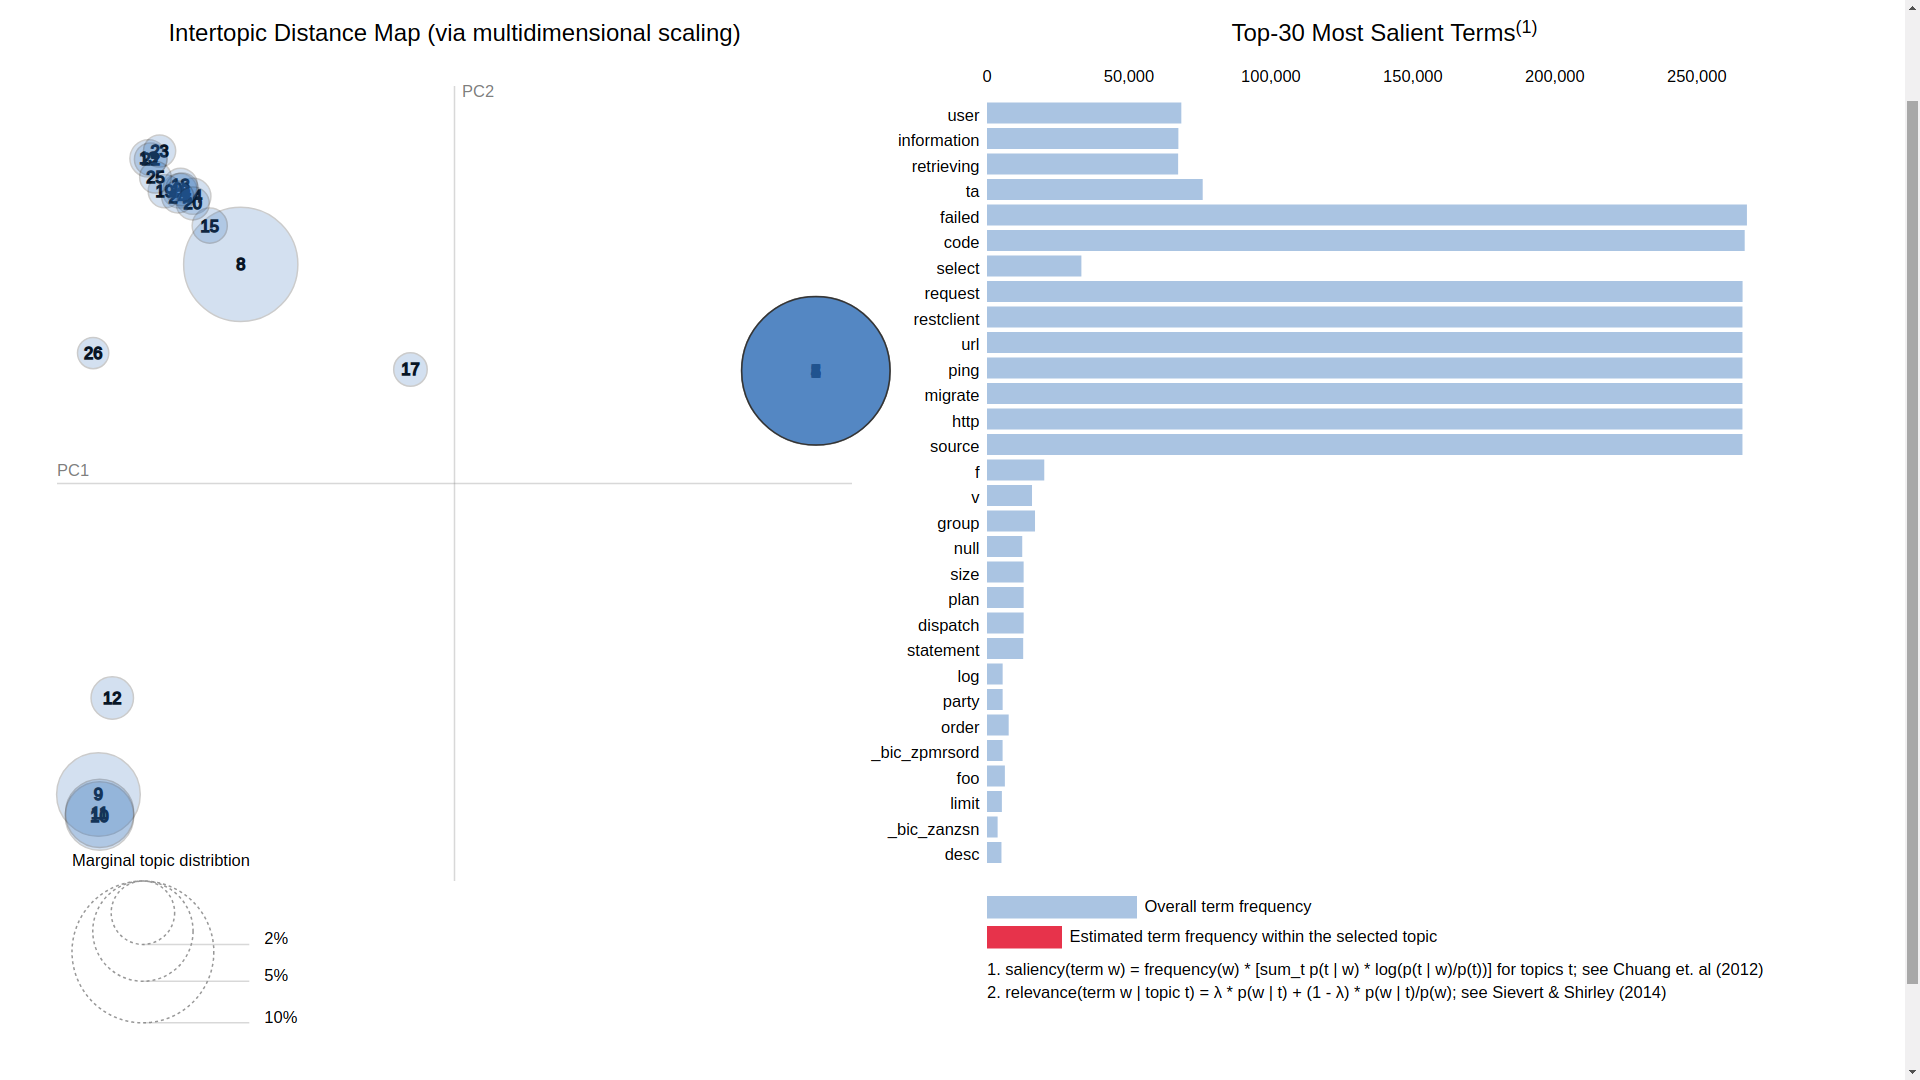
\includegraphics[width=15cm, height=8cm,trim=0 0 100px 0, clip=true]{figures/pyldavis/pyldavis_26.png}
    \caption{PyLdavis topic visualisation with 26 topics}
    \label{fig:pyldavis_26}
\end{figure}

 \begin{figure}[!h]
    \centering
    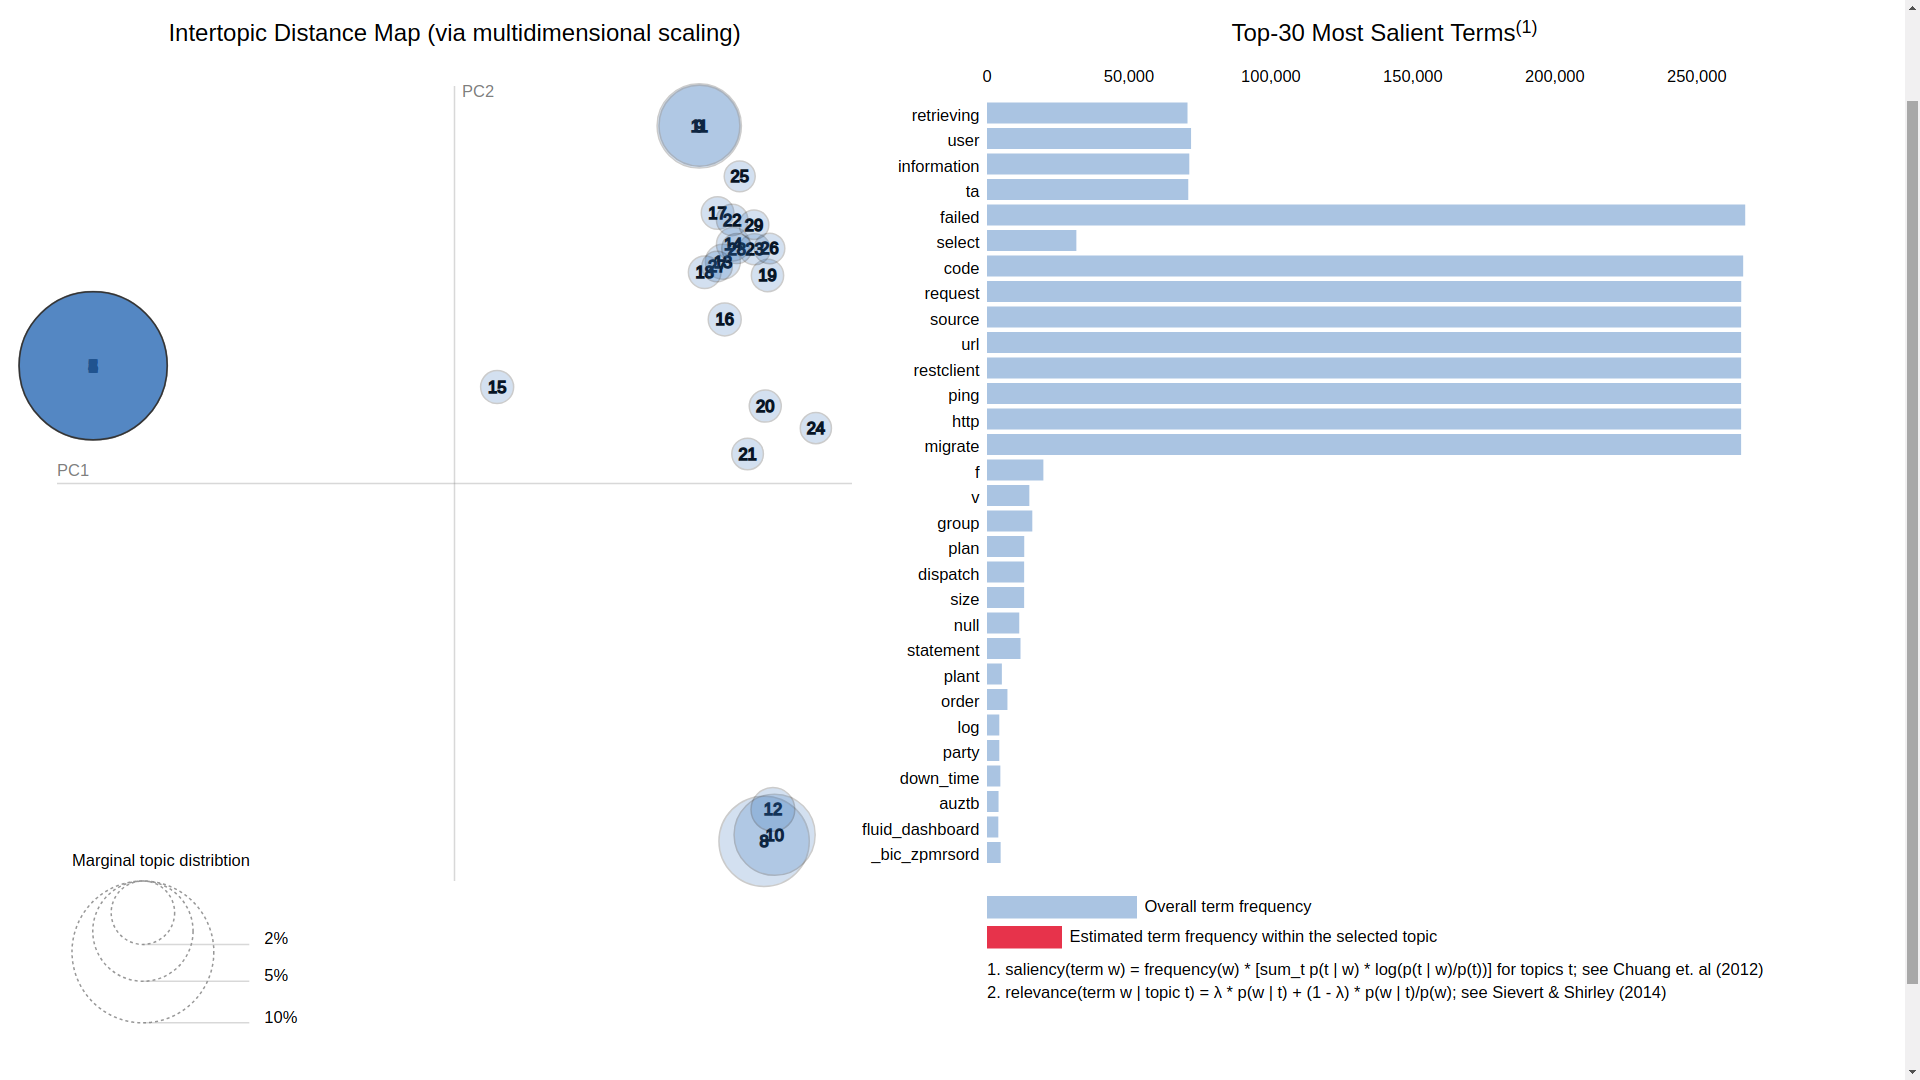
\includegraphics[width=15cm, height=8cm,trim=0 0 100px 0, clip=true]{figures/pyldavis/pyldavis_29.png}
    \caption{PyLdavis topic visualisation with 29 topics}
    \label{fig:pyldavis_29}
\end{figure}

 \begin{figure}[!h]
    \centering
    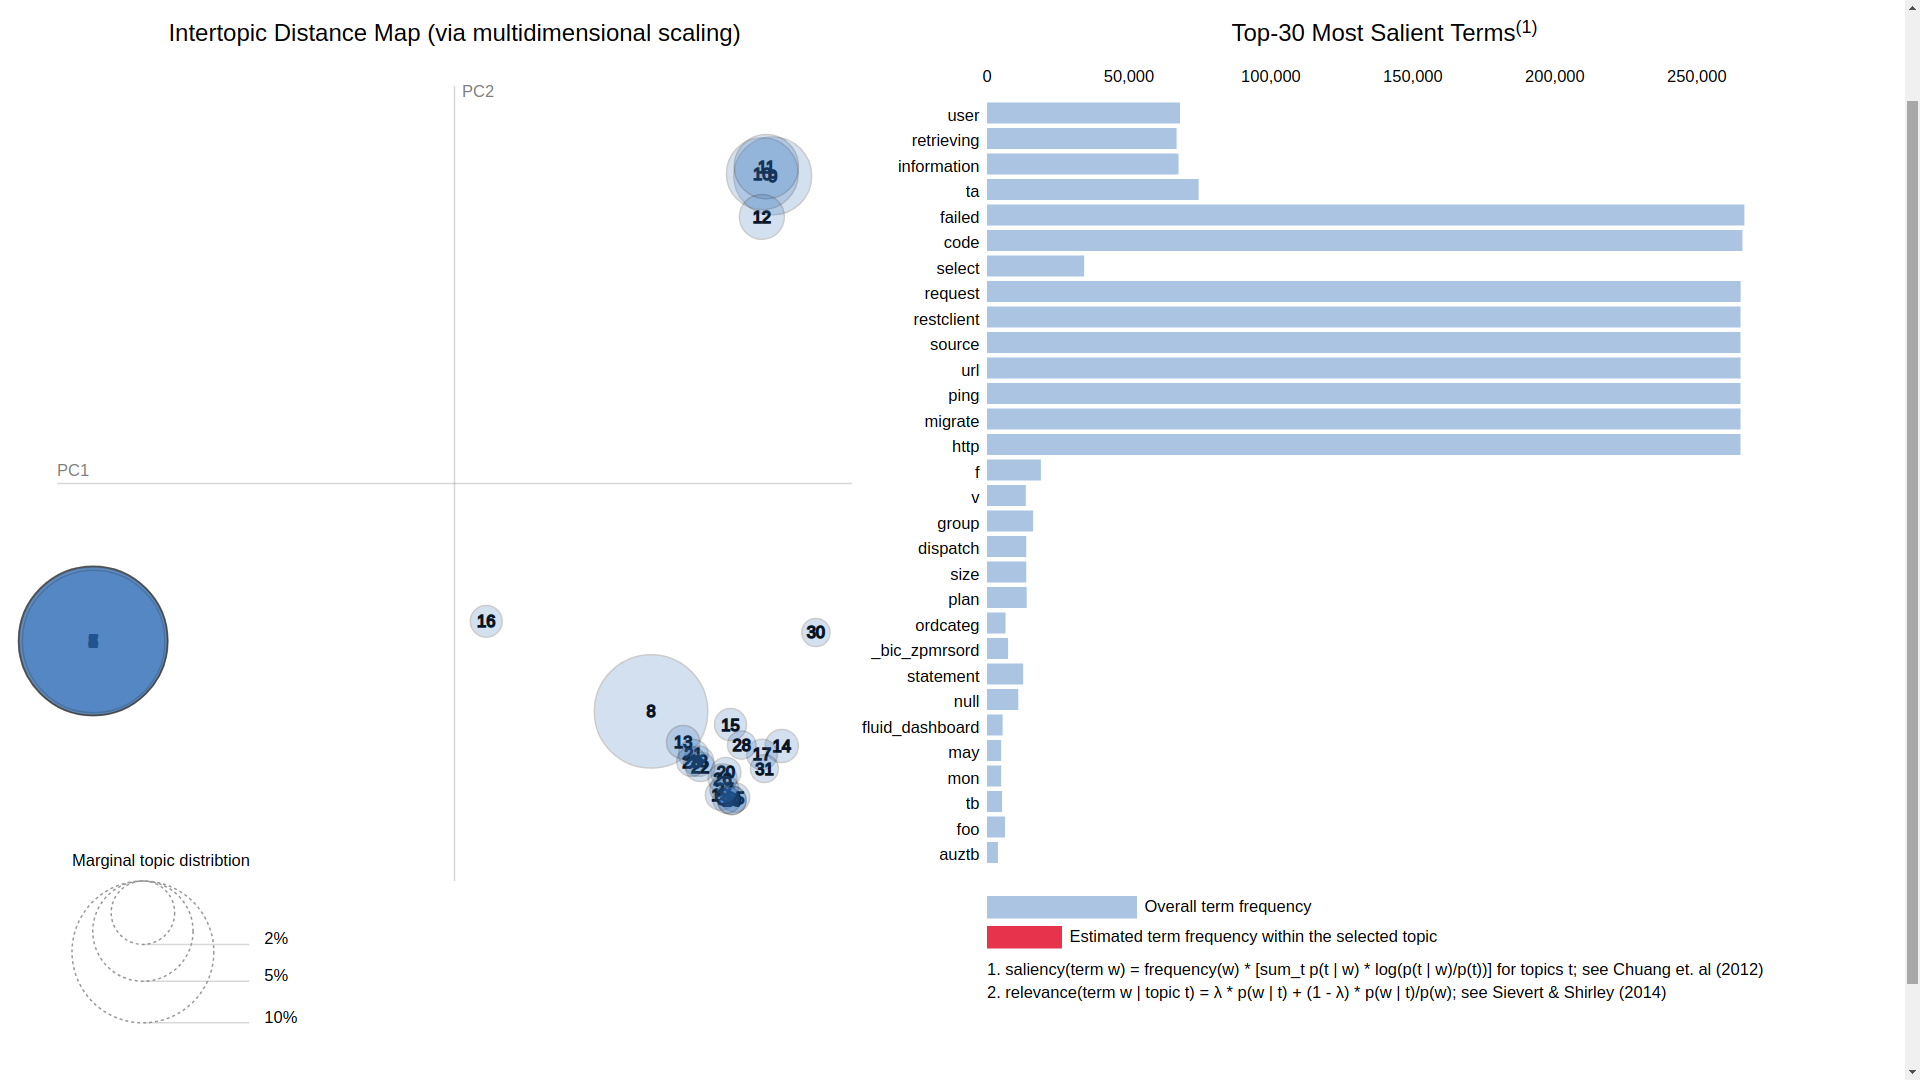
\includegraphics[width=15cm, height=8cm,trim=0 0 100px 0, clip=true]{figures/pyldavis/pyldavis_32.png}
    \caption{PyLdavis topic visualisation with 32 topics}
    \label{fig:pyldavis_32}
\end{figure}

 \begin{figure}[!h]
    \centering
    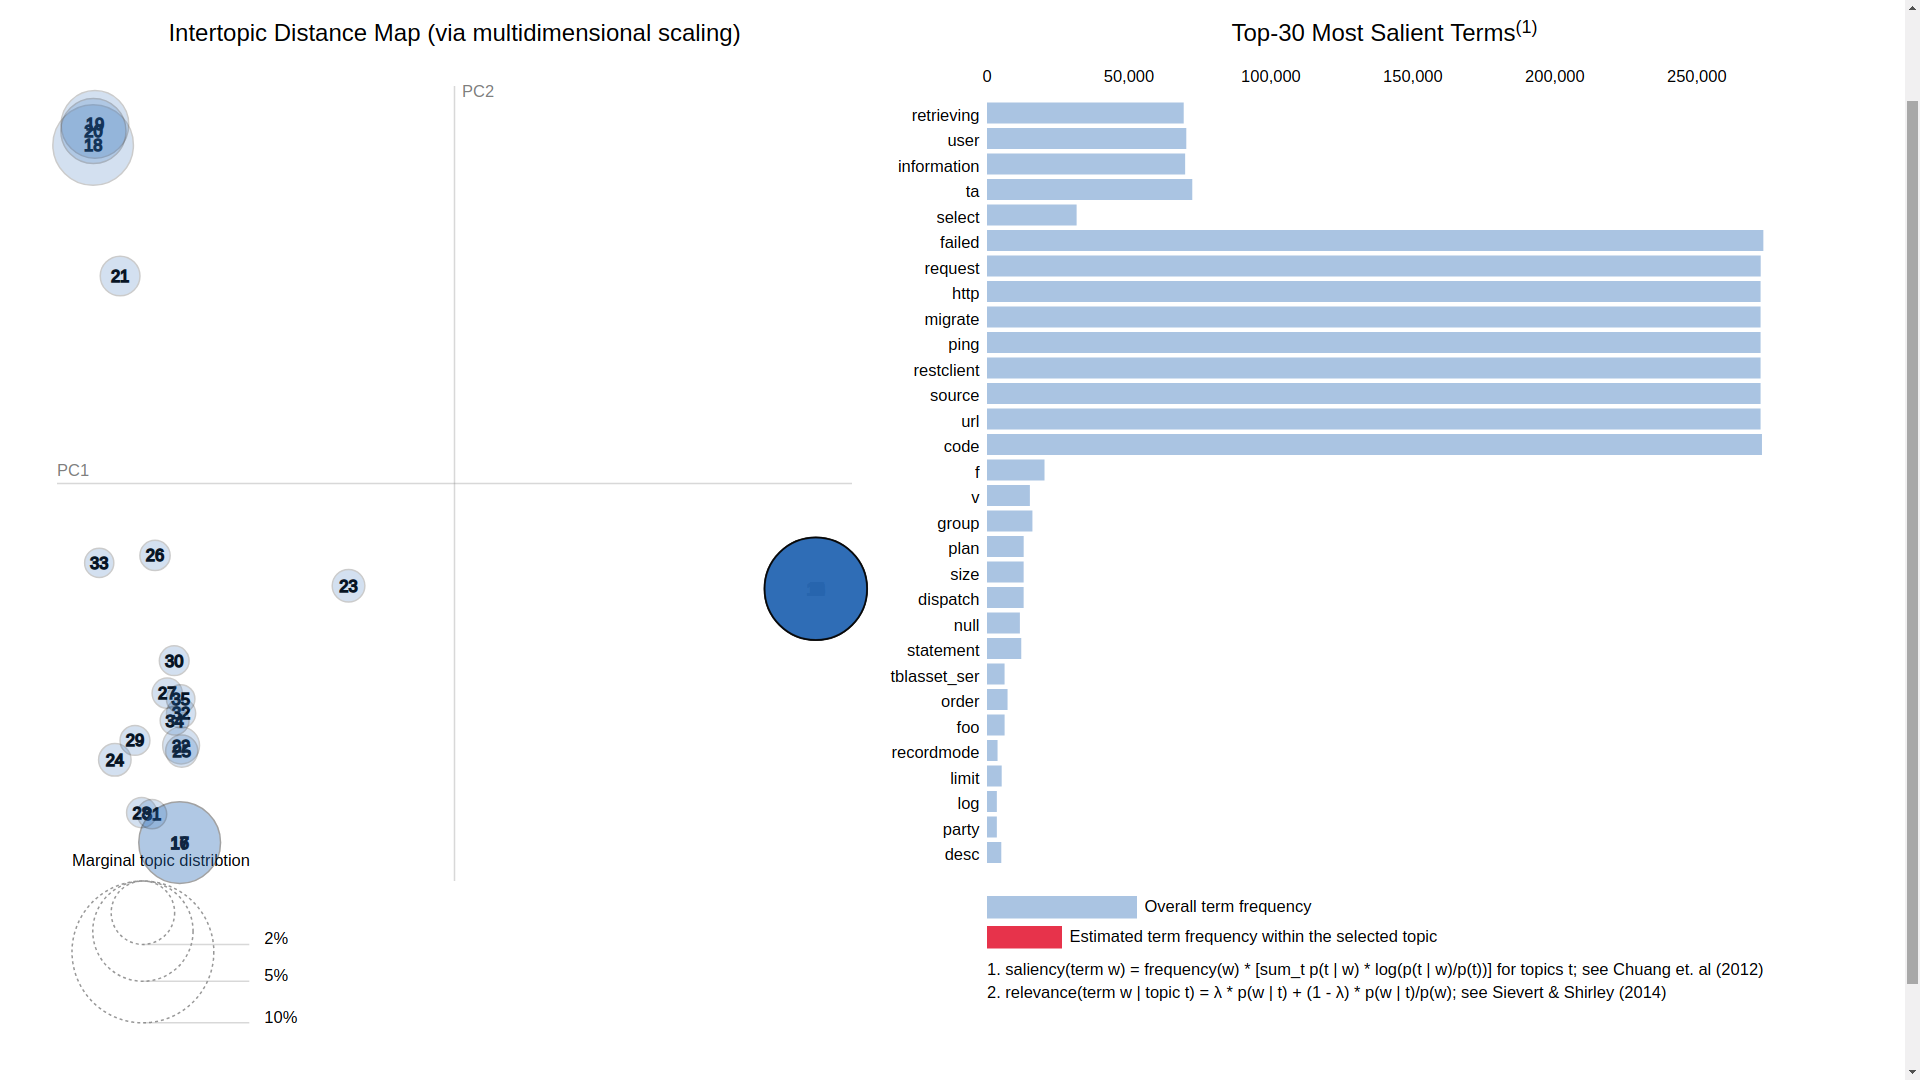
\includegraphics[width=15cm, height=8cm,trim=0 0 100px 0, clip=true]{figures/pyldavis/pyldavis_35.png}
    \caption{PyLdavis topic visualisation with 35 topics}
    \label{fig:pyldavis_35}
\end{figure}

 \begin{figure}[!h]
    \centering
    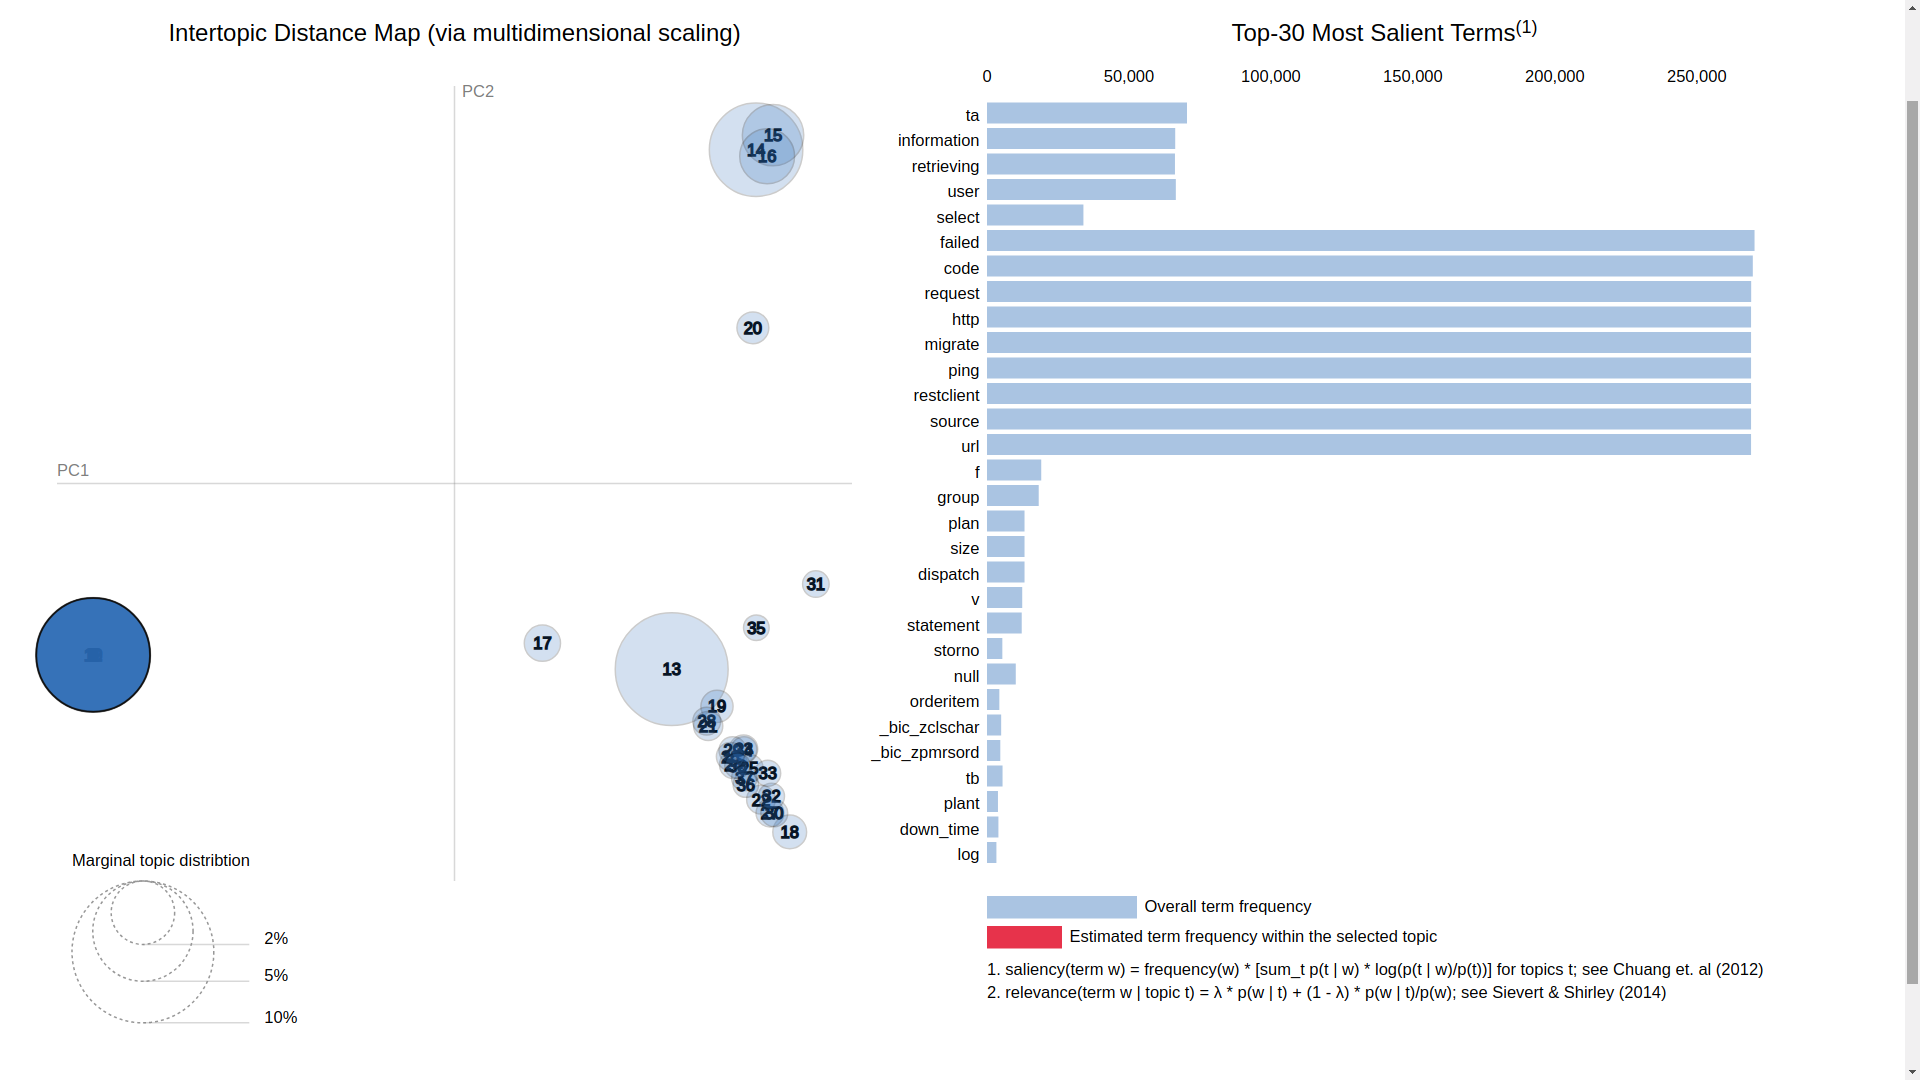
\includegraphics[width=15cm, height=8cm,trim=0 0 100px 0, clip=true]{figures/pyldavis/pyldavis_38.png}
    \caption{PyLdavis topic visualisation with 38 topics}
    \label{fig:pyldavis_38}
\end{figure}

\FloatBarrier
\section{Document distributions per amount of topics}\label{appendices:documentdistribution}

\subsection{Train test}
\begin{figure}[h]
    \centering
    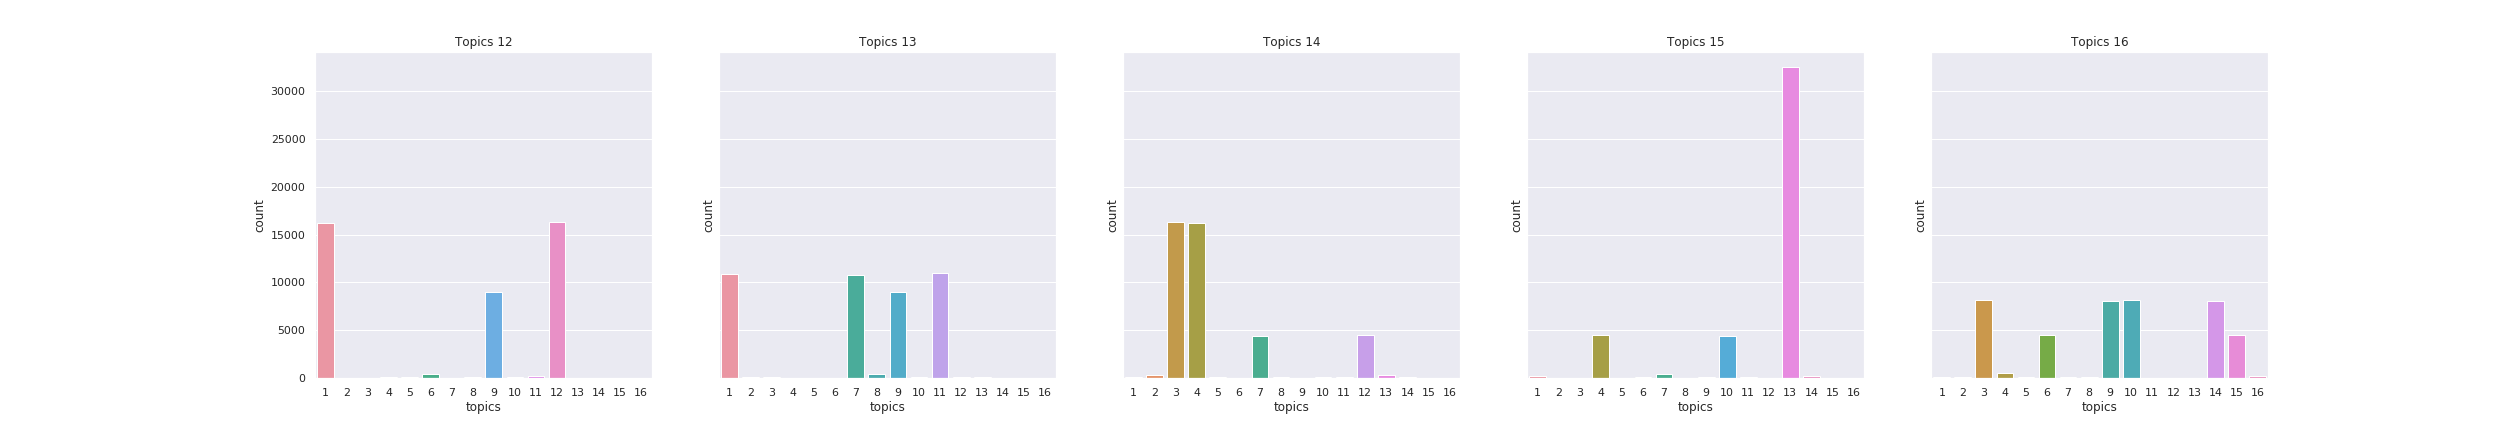
\includegraphics[width=15cm, height=8cm]{figures/doc_distr/doc_distribution_12-16.png}
    \caption{Document distribution with 12-16 topics}
    \label{fig:Doc_distr_12-16corpus}
\end{figure}

\begin{figure}[h]
    \centering
    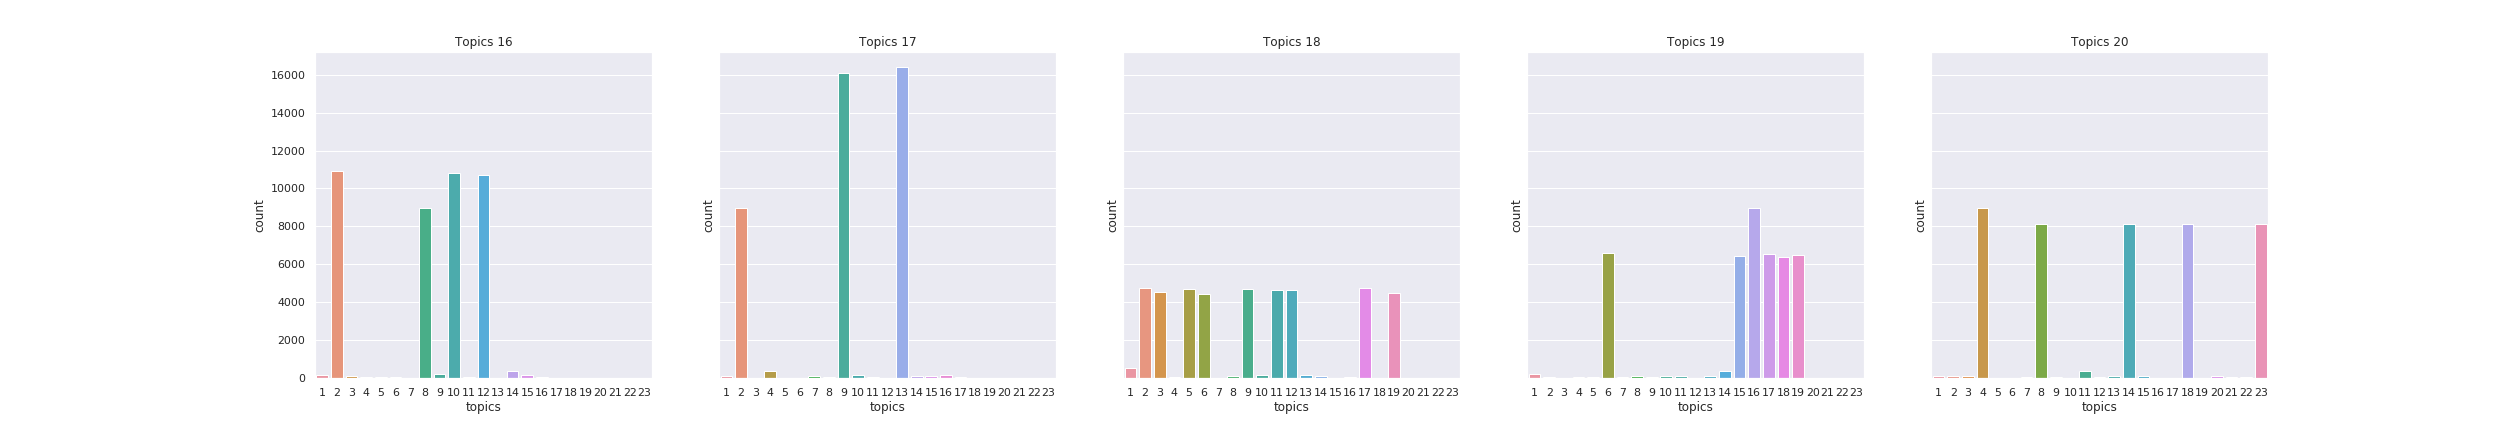
\includegraphics[width=15cm, height=8cm]{figures/doc_distr/doc_distribution_17-23.png}
    \caption{Document distribution with 17-23 topics}
    \label{fig:Doc_distr_17-21corpus}
\end{figure}

\begin{figure}[h]
    \centering
    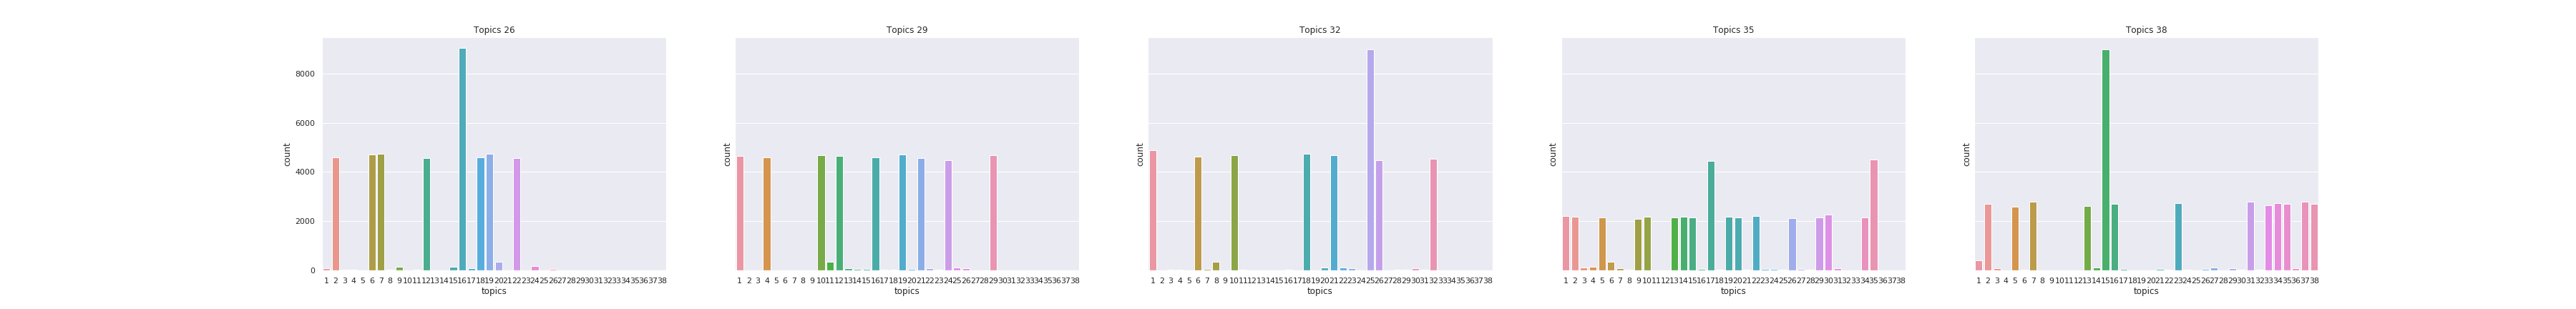
\includegraphics[width=15cm, height=8cm]{figures/doc_distr/doc_distribution_26-38.png}
    \caption{Document distribution with 26-38 topics}
    \label{fig:Doc_distr_26-38corpus}
\end{figure}

\FloatBarrier

\subsection{Held out}
\begin{figure}[h]
    \centering
    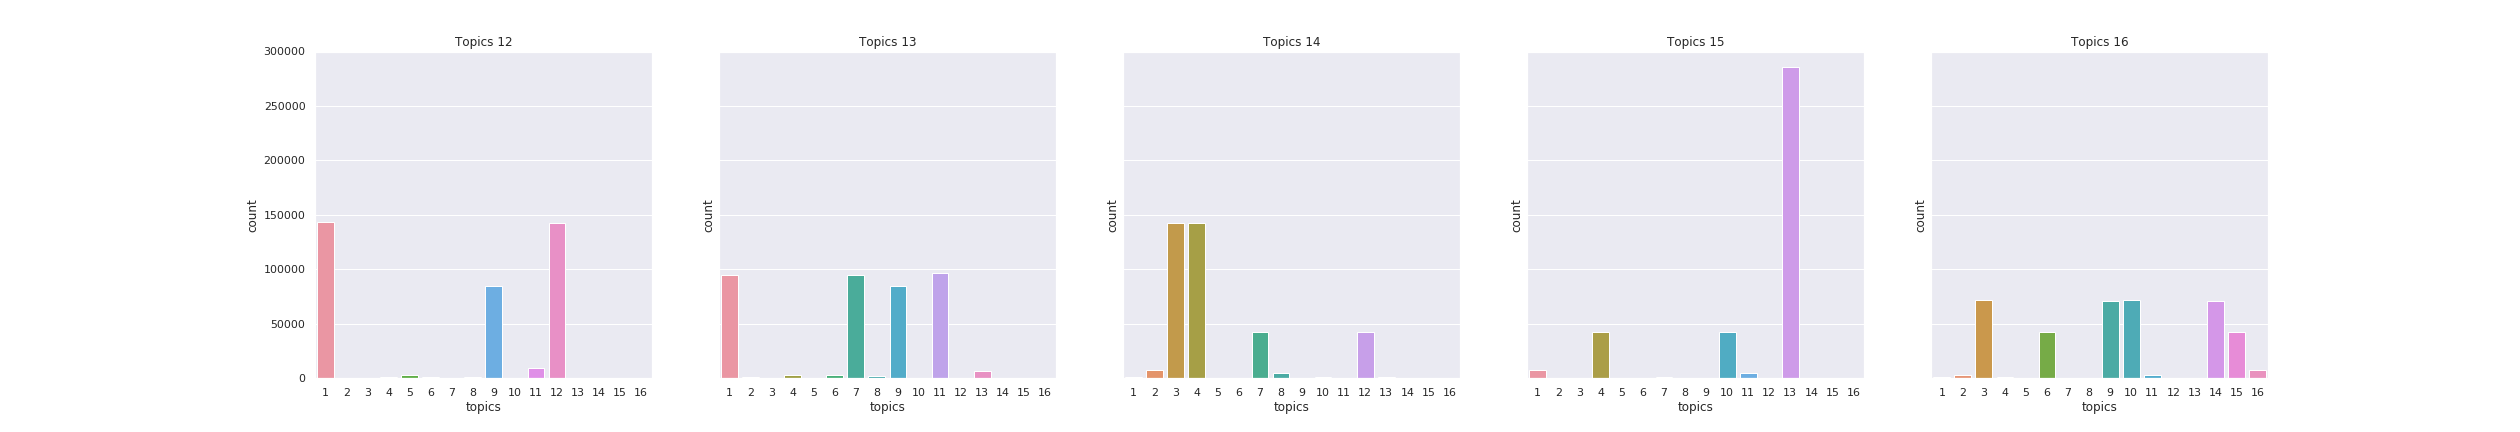
\includegraphics[width=15cm, height=8cm]{figures/doc_distr/doc_distribution_12-16_corpus.png}
    \caption{Document distribution with 12-16 topics}
    \label{fig:Doc_distr_12-16heldout}
\end{figure}

\begin{figure}[h]
    \centering
    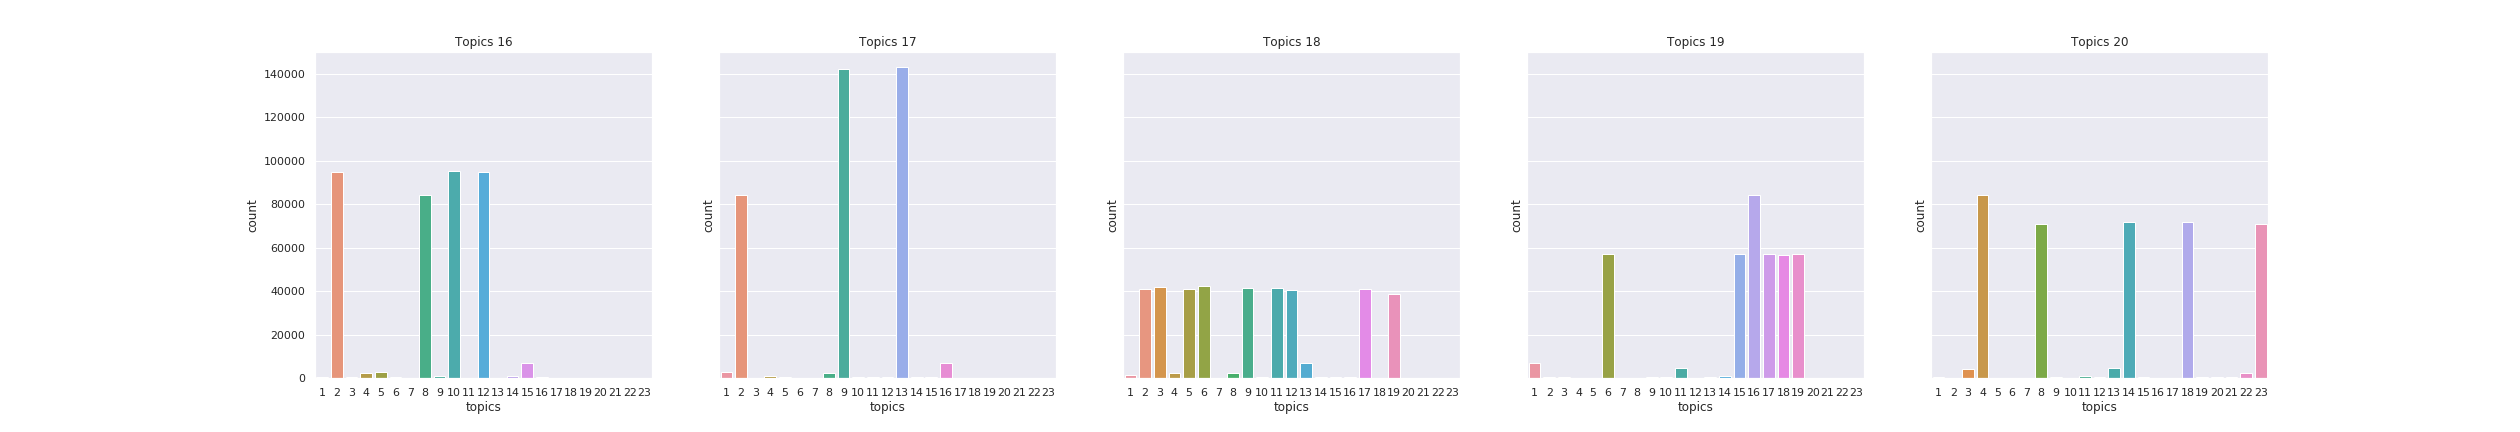
\includegraphics[width=15cm, height=8cm]{figures/doc_distr/doc_distribution_17-23_corpus.png}
    \caption{Document distribution with 17-23 topics}
    \label{fig:Doc_distr_17-21heldout}
\end{figure}

\begin{figure}[h]
    \centering
    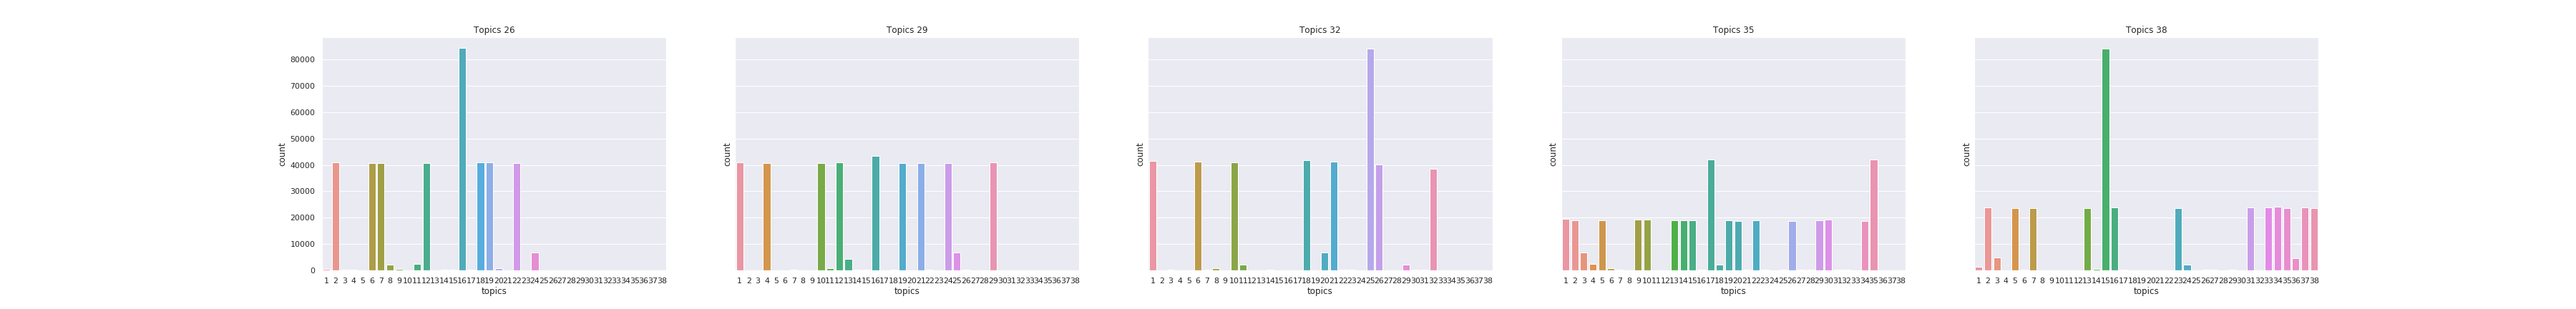
\includegraphics[width=15cm, height=8cm]{figures/doc_distr/doc_distribution_26-38_corpus.png}
    \caption{Document distribution with 26-38 topics}
    \label{fig:Doc_distr_26-38heldout}
\end{figure}

\FloatBarrier
\section{Model topic overview}\label{appendices:modelgeneratedtopics}

\begin{table}[h]
\centering
\begin{tabular}{|l|l|l|l|l|l|}
 \hline
 Topic & Terms & & & & \\
 \hline
 \hline
 0 & user & information & retrieving & ta & select\\ 
 \hline 
 1 & failed & code & request & restclient & ping\\ 
 \hline 
\end{tabular}
\caption{Topic 1..2 with top 5 terms}
\label{tab:appendix2topicsmodel}
\end{table}

\begin{table}[!htb]
\centering
\begin{tabular}{|l|l|l|l|l|l|}
 \hline
 Topic & Terms & & & & \\
 \hline
 0 & failed & code & request & source & ping\\ 
 \hline 
 1 & ta & select & f & group & plan\\ 
 \hline 
 2 & user & information & retrieving & text & log\\ 
 \hline 
\end{tabular}
\caption{Topic 1..3 with top 5 terms}
\label{tab:3topicsmodel}
\end{table}
 
\begin{table}[!htb]
\centering
\begin{tabular}{|l|l|l|l|l|l|}
 \hline
 Topic & Terms & & & & \\
 \hline
 0 & fluid\_dashboard & text & tblasset\_ser & recordmode & log\\ 
 \hline 
 1 & ta & select & f & group & plan\\ 
 \hline 
 2 & user & information & retrieving & cancel & token\\ 
 \hline 
 3 & failed & code & request & source & restclient\\ 
 \hline 
\end{tabular}
\caption{Topic 1..4 with top 5 terms}
\label{tab:4topicsmodel}
\end{table}
 
\begin{table}[h]
\centering
\begin{tabular}{|l|l|l|l|l|l|}
 \hline
 Topic & Terms & & & & \\
 \hline
 \hline
 0 & ta & select & f & group & plan\\ 
 \hline 
 1 & fluid\_dashboard & text & tblasset\_ser & tbljob\_sow & group\\ 
 \hline 
 2 & v & r & order & null & tb\\ 
 \hline 
 3 & failed & code & request & source & restclient\\ 
 \hline 
 4 & user & information & retrieving & log & party\\ 
 \hline 
\end{tabular}
\caption{Topic 1..5 with top 5 terms}
\label{tab:appendix5topicsmodel}
\end{table}
 
\begin{table}[!htb]
\centering
\begin{tabular}{|l|l|l|l|l|l|}
 \hline
 Topic & Terms & & & & \\
 \hline
 0 & failed & code & request & source & url\\ 
 \hline 
 1 & fluid\_dashboard & text & tblasset\_ser & tbljob\_sow & coord\_type\\ 
 \hline 
 2 & user & information & retrieving & controller & could\\ 
 \hline 
 3 & count & plant & redo & customer & record\\ 
 \hline 
 4 & ta & select & f & group & plan\\ 
 \hline 
 5 & v & order & r & null & tb\\ 
 \hline 
\end{tabular}
\caption{Topic 1..6 with top 5 terms}
\label{tab:6topicsmodel}
\end{table}
 
\begin{table}[!htb]
\centering
\begin{tabular}{|l|l|l|l|l|l|}
 \hline
 Topic & Terms & & & & \\
 \hline
 0 & ta & select & size & dispatch & plan\\ 
 \hline 
 1 & notificatn & coord\_type & rowcnt & tblasset\_ser & \_bic\_zvorgang\\ 
 \hline 
 2 & user & information & retrieving & terminated & slice\_id\\ 
 \hline 
 3 & f & v & group & limit & desc\\ 
 \hline 
 4 & fluid\_dashboard & text & tblasset\_ser & tbljob\_sow & orderitem\\ 
 \hline 
 5 & v & r & order & tb & null\\ 
 \hline 
 6 & failed & code & request & url & source\\ 
 \hline 
\end{tabular}
\caption{Topic 1..7 with top 5 terms}
\label{tab:7topicsmodel}
\end{table}
 
\begin{table}[!htb]
\centering
\begin{tabular}{|l|l|l|l|l|l|}
 \hline
 Topic & Terms & & & & \\
 \hline
 0 & request & ping & source & restclient & url\\ 
 \hline 
 1 & log & party & \_bic\_zanzsn & orderitem & \_bic\_zvorgang\\ 
 \hline 
 2 & request & ping & migrate & source & http\\ 
 \hline 
 3 & coord\_type & ordcateg & cancel & token & \_bic\_zpmrsord\\ 
 \hline 
 4 & user & information & retrieving & may & mon\\ 
 \hline 
 5 & ta & select & f & group & plan\\ 
 \hline 
 6 & failed & plant & group & code & controller\\ 
 \hline 
 7 & fluid\_dashboard & text & tblasset\_ser & tbljob\_sow & rowcnt\\ 
 \hline 
\end{tabular}
\caption{Topic 1..8 with top 5 terms}
\label{tab:8topicsmodel}
\end{table}
 
\begin{table}[!htb]
\centering
\begin{tabular}{|l|l|l|l|l|l|}
 \hline
 Topic & Terms & & & & \\
 \hline
 0 & ta & f & group & limit & desc\\ 
 \hline 
 1 & fluid\_dashboard & text & tblasset\_ser & tbljob\_sow & may\\ 
 \hline 
 2 & log & party & coord\_type & storno & employee\\ 
 \hline 
 3 & ta & select & size & dispatch & plan\\ 
 \hline 
 4 & failed & code & request & source & url\\ 
 \hline 
 5 & ordcateg & unit\_day & auztb & ops & hawqstatus\\ 
 \hline 
 6 & user & information & retrieving & terminated & stage\\ 
 \hline 
 7 & cancel & rowcnt & redo & token & record\\ 
 \hline 
 8 & v & r & select & null & order\\ 
 \hline 
\end{tabular}
\caption{Topic 1..9 with top 5 terms}
\label{tab:9topicsmodel}
\end{table}
 
 \begin{table}[h]
\centering
\begin{tabular}{|l|l|l|l|l|l|}
 \hline
 Topic & Terms & & & & \\
 \hline
 \hline
 0 & request & migrate & restclient & url & ping\\ 
 \hline 
 1 & fluid\_dashboard & text & tblasset\_ser & tbljob\_sow & coord\_type\\ 
 \hline 
 2 & ordcateg & cancel & token & postgres & \_bic\_zpmrsord\\ 
 \hline 
 3 & orderitem & redo & record & unit\_day & length\\ 
 \hline 
 4 & f & foo & count & ta & v\\ 
 \hline 
 5 & ops & hawqstatus & down\_indic & set & \_bic\_zlongit\\ 
 \hline 
 6 & request & ping & migrate & url & http\\ 
 \hline 
 7 & failed & material & recordmode & notificatn & group\\ 
 \hline 
 8 & ta & select & group & plan & dispatch\\ 
 \hline 
 9 & user & information & retrieving & tblasset\_ser & tbljob\_sow\\ 
 \hline 
\end{tabular}
\caption{Topic 1..10 with top 5 terms}
\label{tab:appendix10topicsmodel}
\end{table}
 
\begin{table}[!htb]
\centering
\begin{tabular}{|l|l|l|l|l|l|}
 \hline
 Topic & Terms & & & & \\
 \hline
 0 & request & ping & source & restclient & url\\ 
 \hline 
 1 & failed & group & controller & code & could\\ 
 \hline 
 2 & ta & select & plan & dispatch & size\\ 
 \hline 
 3 & \_bic\_zanzsn & orderitem & \_bic\_zvorgang & \_bic\_zpmrsord & set\\ 
 \hline 
 4 & coord\_type & storno & unit\_day & division & employee\\ 
 \hline 
 5 & ta & f & group & v & select\\ 
 \hline 
 6 & request & source & url & restclient & code\\ 
 \hline 
 7 & user & information & retrieving & tblasset\_ser & tbljob\_sow\\ 
 \hline 
 8 & ta & v & select & null & r\\ 
 \hline 
 9 & plant & redo & customer & record & length\\ 
 \hline 
 10 & fluid\_dashboard & text & tblasset\_ser & log & party\\ 
 \hline 
\end{tabular}
\caption{Topic 1..11 with top 5 terms}
\label{tab:11topicsmodel}
\end{table}
 
\begin{table}[!htb]
\centering
\begin{tabular}{|l|l|l|l|l|l|}
 \hline
 Topic & Terms & & & & \\
 \hline
 0 & request & ping & migrate & source & http\\ 
 \hline 
 1 & plant & redo & customer & record & length\\ 
 \hline 
 2 & ordcateg & unit\_day & notif\_orgn & down\_time & auztv\\ 
 \hline 
 3 & failed & controller & group & code & could\\ 
 \hline 
 4 & ta & f & order & v & null\\ 
 \hline 
 5 & fluid\_dashboard & text & log & party & tblasset\_ser\\ 
 \hline 
 6 & ta & material & recordmode & notificatn & createdon\\ 
 \hline 
 7 & tblasset\_ser & cancel & tbljob\_sow & orderitem & token\\ 
 \hline 
 8 & information & user & retrieving & \_bic\_zpmrsord & \_bic\_zobjvw\\ 
 \hline 
 9 & \_bic\_zanzsn & coord\_type & may & mon & \_bic\_zvorgang\\ 
 \hline 
 10 & ta & select & group & plan & dispatch\\ 
 \hline 
 11 & request & ping & source & restclient & url\\ 
 \hline 
\end{tabular}
\caption{Topic 1..12 with top 5 terms}
\label{tab:12topicsmodel}
\end{table}
 
\begin{table}[!htb]
\centering
\begin{tabular}{|l|l|l|l|l|l|}
 \hline
 Topic & Terms & & & & \\
 \hline
 0 & request & ping & url & source & restclient\\ 
 \hline 
 1 & failed & group & controller & code & could\\ 
 \hline 
 2 & cancel & token & postgres & auztb & user\\ 
 \hline 
 3 & ta & f & v & order & null\\ 
 \hline 
 4 & coord\_type & rowcnt & storno & unit\_day & division\\ 
 \hline 
 5 & ta & f & select & v & group\\ 
 \hline 
 6 & request & ping & url & source & restclient\\ 
 \hline 
 7 & fluid\_dashboard & text & tblasset\_ser & log & party\\ 
 \hline 
 8 & information & retrieving & user & \_bic\_zpmrsord & \_bic\_zobjvw\\ 
 \hline 
 9 & \_bic\_zanzsn & \_bic\_zvorgang & \_bic\_zqmdat & \_bic\_zbautl\_hd & set\\ 
 \hline 
 10 & request & code & failed & source & restclient\\ 
 \hline 
 11 & redo & record & length & checkpoint & restart\\ 
 \hline 
 12 & ta & select & plan & dispatch & size\\ 
 \hline 
\end{tabular}
\caption{Topic 1..13 with top 5 terms}
\label{tab:13topicsmodel}
\end{table}
 
\begin{table}[!htb]
\centering
\begin{tabular}{|l|l|l|l|l|l|}
 \hline
 Topic & Terms & & & & \\
 \hline
 0 & failed & group & controller & code & could\\ 
 \hline 
 1 & ta & select & plan & dispatch & size\\ 
 \hline 
 2 & request & restclient & failed & source & code\\ 
 \hline 
 3 & request & restclient & url & source & failed\\ 
 \hline 
 4 & fluid\_dashboard & text & recordmode & \_bic\_zanzsn & \_bic\_zvorgang\\ 
 \hline 
 5 & v & ta & select & r & null\\ 
 \hline 
 6 & information & retrieving & user & \_bic\_zpmrsord & \_bic\_zobjvw\\ 
 \hline 
 7 & ta & f & select & group & v\\ 
 \hline 
 8 & ta & unit\_day & auztb & \_bic\_zpmrsord & division\\ 
 \hline 
 9 & cancel & rowcnt & token & postgres & user\\ 
 \hline 
 10 & tblasset\_ser & coord\_type & tbljob\_sow & storno & down\_indic\\ 
 \hline 
 11 & information & user & retrieving & \_bic\_zpmrsord & \_bic\_zobjvw\\ 
 \hline 
 12 & log & party & mat\_plant & p\_plant & \_bic\_zpsttr\\ 
 \hline 
 13 & ordcateg & redo & record & length & checkpoint\\ 
 \hline 
\end{tabular}
\caption{Topic 1..14 with top 5 terms}
\label{tab:14topicsmodel}
\end{table}
 
\begin{table}[!htb]
\centering
\begin{tabular}{|l|l|l|l|l|l|}
 \hline
 Topic & Terms & & & & \\
 \hline
 0 & ta & select & plan & dispatch & size\\ 
 \hline 
 1 & \_bic\_zanzsn & \_bic\_zvorgang & record & length & checkpoint\\ 
 \hline 
 2 & ta & material & recordmode & notificatn & \_bic\_zobzae\\ 
 \hline 
 3 & information & retrieving & user & \_bic\_zpmrsord & down\_time\\ 
 \hline 
 4 & ordcateg & class\_num & order\_quan & class\_type & \_bic\_zangeb\\ 
 \hline 
 5 & orderitem & not\_type & notif\_orgn & \_bic\_zbautl\_hd & ausbs\\ 
 \hline 
 6 & log & party & cancel & token & postgres\\ 
 \hline 
 7 & plant & customer & wbs\_elemt & redo & costcenter\\ 
 \hline 
 8 & fluid\_dashboard & text & tblasset\_ser & tbljob\_sow & auztb\\ 
 \hline 
 9 & user & retrieving & information & \_bic\_zpmrsord & proxy\\ 
 \hline 
 10 & ta & f & group & select & v\\ 
 \hline 
 11 & set & search\_path & saperrorcode & saperrormessage & job\_guid\\ 
 \hline 
 12 & failed & code & request & source & url\\ 
 \hline 
 13 & may & mon & employee & quantity & amountfx\\ 
 \hline 
 14 & coord\_type & ta & down\_time & storno & \_bic\_zpmrsord\\ 
 \hline 
\end{tabular}
\caption{Topic 1..15 with top 5 terms}
\label{tab:15topicsmodel}
\end{table}
 
\begin{table}[!htb]
\centering
\begin{tabular}{|l|l|l|l|l|l|}
 \hline
 Topic & Terms & & & & \\
 \hline
 0 & v & r & select & order & null\\ 
 \hline 
 1 & ta & f & select & foo & v\\ 
 \hline 
 2 & failed & code & source & restclient & url\\ 
 \hline 
 3 & log & party & coord\_type & rowcnt & may\\ 
 \hline 
 4 & unit\_day & employee & quantity & amount & amountvr\\ 
 \hline 
 5 & information & retrieving & user & \_bic\_zpmrsord & down\_time\\ 
 \hline 
 6 & cancel & token & tbljob\_sow & postgres & tblasset\_ser\\ 
 \hline 
 7 & fluid\_dashboard & text & \_bic\_zanzsn & tblasset\_ser & \_bic\_zvorgang\\ 
 \hline 
 8 & failed & code & request & source & url\\ 
 \hline 
 9 & failed & code & request & http & ping\\ 
 \hline 
 10 & ta & f & limit & v & desc\\ 
 \hline 
 11 & orderitem & tblasset\_ser & \_bic\_zpmrsord & class\_type & class\_num\\ 
 \hline 
 12 & \_bic\_zqmdat & \_bic\_zbautl\_hd & set & \_bic\_znummanf & \_bic\_znumsgpw\\ 
 \hline 
 13 & failed & code & request & url & source\\ 
 \hline 
 14 & information & user & retrieving & side & extension\\ 
 \hline 
 15 & ta & select & size & dispatch & plan\\ 
 \hline 
\end{tabular}
\caption{Topic 1..16 with top 5 terms}
\label{tab:16topicsmodel}
\end{table}
 
\begin{table}[!htb]
\centering
\begin{tabular}{|l|l|l|l|l|l|}
 \hline
 Topic & Terms & & & & \\
 \hline
 0 & ordcateg & cancel & token & postgres & hdfs\\ 
 \hline 
 1 & request & url & failed & source & restclient\\ 
 \hline 
 2 & fluid\_dashboard & text & tblasset\_ser & tbljob\_sow & down\_indic\\ 
 \hline 
 3 & ta & f & limit & v & desc\\ 
 \hline 
 4 & ta & f & select & v & foo\\ 
 \hline 
 5 & plant & redo & record & length & checkpoint\\ 
 \hline 
 6 & coord\_type & down\_time & storno & \_bic\_zclschar & \_bic\_zsystatus\\ 
 \hline 
 7 & user & retrieving & information & first & without\\ 
 \hline 
 8 & rowcnt & may & mon & ops & hawqstatus\\ 
 \hline 
 9 & request & ping & source & code & failed\\ 
 \hline 
 10 & \_bic\_zanzsn & \_bic\_zvorgang & \_bic\_znumsgpw & \_bic\_zlatit & \_bic\_zlongit\\ 
 \hline 
 11 & restclient & ping & source & failed & code\\ 
 \hline 
 12 & unit\_day & division & \_bic\_zgsmng & \_bic\_zangeb & \_bic\_zbedarf\\ 
 \hline 
 13 & log & party & not\_type & notif\_orgn & ausvn\\ 
 \hline 
 14 & ta & select & plan & dispatch & size\\ 
 \hline 
 15 & failed & controller & code & could & details\\ 
 \hline 
 16 & orderitem & \_bic\_zpmrsord & class\_num & class\_type & partno\\ 
 \hline 
\end{tabular}
\caption{Topic 1..17 with top 5 terms}
\label{tab:17topicsmodel}
\end{table}
 
\begin{table}[!htb]
\centering
\begin{tabular}{|l|l|l|l|l|l|}
 \hline
 Topic & Terms & & & & \\
 \hline
 0 & ta & f & select & v & foo\\ 
 \hline 
 1 & information & user & retrieving & \_bic\_zpmrsord & proxy\\ 
 \hline 
 2 & ta & not\_type & notif\_orgn & unit\_day & ausbs\\ 
 \hline 
 3 & log & party & ordcateg & po\_unit & ord\_typ\\ 
 \hline 
 4 & v & select & r & ta & null\\ 
 \hline 
 5 & orderitem & division & zzwbs & zzdber & equnr\\ 
 \hline 
 6 & may & mon & class\_num & class\_type & e\\ 
 \hline 
 7 & ta & f & group & limit & desc\\ 
 \hline 
 8 & failed & code & request & url & restclient\\ 
 \hline 
 9 & auztb & client & eof & sales\_unit & n\\ 
 \hline 
 10 & plant & redo & customer & record & length\\ 
 \hline 
 11 & \_bic\_zanzsn & \_bic\_zvorgang & down\_indic & \_bic\_zlongit & \_bic\_znumsgpw\\ 
 \hline 
 12 & failed & code & request & source & restclient\\ 
 \hline 
 13 & fluid\_dashboard & text & rowcnt & tblasset\_ser & time\\ 
 \hline 
 14 & cancel & token & postgres & user & hdfs\\ 
 \hline 
 15 & ta & select & plan & dispatch & size\\ 
 \hline 
 16 & tblasset\_ser & tbljob\_sow & ops & hawqstatus & saperrorcode\\ 
 \hline 
 17 & coord\_type & \_bic\_zpmrsord & storno & down\_time & \_bic\_zclschar\\ 
 \hline 
\end{tabular}
\caption{Topic 1..18 with top 5 terms}
\label{tab:18topicsmodel}
\end{table}
 
\begin{table}[!htb]
\centering
\begin{tabular}{|l|l|l|l|l|l|}
 \hline
 Topic & Terms & & & & \\
 \hline
 0 & fluid\_dashboard & text & log & party & rowcnt\\ 
 \hline 
 1 & request & restclient & failed & source & code\\ 
 \hline 
 2 & information & retrieving & user & \_bic\_zpmrsord & down\_time\\ 
 \hline 
 3 & ta & f & select & v & foo\\ 
 \hline 
 4 & restclient & ping & source & failed & code\\ 
 \hline 
 5 & information & retrieving & user & \_bic\_zpmrsord & down\_time\\ 
 \hline 
 6 & \_bic\_zanzsn & \_bic\_zvorgang & down\_indic & \_bic\_zlatit & \_bic\_znummanf\\ 
 \hline 
 7 & ta & f & limit & desc & order\\ 
 \hline 
 8 & code & ping & source & url & restclient\\ 
 \hline 
 9 & unit\_day & \_bic\_zpmrsord & client & eof & n\\ 
 \hline 
 10 & request & ping & source & code & failed\\ 
 \hline 
 11 & request & ping & source & restclient & failed\\ 
 \hline 
 12 & ta & select & plan & size & dispatch\\ 
 \hline 
 13 & failed & controller & group & code & could\\ 
 \hline 
 14 & v & ta & select & r & null\\ 
 \hline 
 15 & redo & record & length & checkpoint & restart\\ 
 \hline 
 16 & restclient & ping & source & failed & code\\ 
 \hline 
 17 & tblasset\_ser & createdon & assembly & tbljob\_sow & orderitem\\ 
 \hline 
 18 & request & failed & url & source & restclient\\ 
 \hline 
\end{tabular}
\caption{Topic 1..19 with top 5 terms}
\label{tab:19topicsmodel}
\end{table}
 
\begin{table}[!htb]
\centering
\begin{tabular}{|l|l|l|l|l|l|}
 \hline
 Topic & Terms & & & & \\
 \hline
 0 & ta & select & statement & plan & size\\ 
 \hline 
 1 & redo & record & length & checkpoint & restart\\ 
 \hline 
 2 & v & r & select & order & null\\ 
 \hline 
 3 & fluid\_dashboard & text & tblasset\_ser & tbljob\_sow & down\_indic\\ 
 \hline 
 4 & failed & group & material & equipment & recordmode\\ 
 \hline 
 5 & request & ping & source & code & failed\\ 
 \hline 
 6 & terminated & stage & search & cest & stack\_trace\\ 
 \hline 
 7 & may & mon & \_bic\_zqmdat & \_bic\_znumsgpw & \_bic\_zlongit\\ 
 \hline 
 8 & orderitem & \_bic\_zpmrsord & ops & hawqstatus & dispatch\\ 
 \hline 
 9 & ordcateg & unit\_day & auztb & client & eof\\ 
 \hline 
 10 & ta & f & select & v & group\\ 
 \hline 
 11 & not\_type & notif\_orgn & storno & ausbs & ausvn\\ 
 \hline 
 12 & cancel & token & postgres & delegation & hdfs\\ 
 \hline 
 13 & log & party & \_bic\_zanzsn & rowcnt & \_bic\_zvorgang\\ 
 \hline 
 14 & request & restclient & url & source & code\\ 
 \hline 
 15 & user & information & retrieving & simpleajpservice & e\\ 
 \hline 
 16 & request & ping & source & code & failed\\ 
 \hline 
 17 & code & ping & source & failed & restclient\\ 
 \hline 
 18 & request & ping & source & code & failed\\ 
 \hline 
 19 & coord\_type & without & employee & quantity & quantityfx\\ 
 \hline 
\end{tabular}
\caption{Topic 1..20 with top 5 terms}
\label{tab:20topicsmodel}
\end{table}
 
\begin{table}[!htb]
\centering
\begin{tabular}{|l|l|l|l|l|l|}
 \hline
 Topic & Terms & & & & \\
 \hline
 0 & redo & record & checkpoint & length & restart\\ 
 \hline 
 1 & \_bic\_zobknr & assembly & rowcnt & may & mon\\ 
 \hline 
 2 & ta & select & group & f & foo\\ 
 \hline 
 3 & information & user & retrieving & without & first\\ 
 \hline 
 4 & not\_type & notif\_orgn & storno & oi\_ebelp & mat\_plant\\ 
 \hline 
 5 & auztb & class\_type & class\_num & job\_guid & \_bic\_zperidint\\ 
 \hline 
 6 & fluid\_dashboard & text & \_bic\_zanzsn & \_bic\_zvorgang & down\_indic\\ 
 \hline 
 7 & request & url & code & source & restclient\\ 
 \hline 
 8 & failed & controller & could & code & policy\\ 
 \hline 
 9 & \_bic\_zqmdat & saperrormessage & saperrorcode & sapstatus & partno\\ 
 \hline 
 10 & log & party & po\_unit & \_bic\_zcslngtxt & \_bic\_zrev\_lvl\\ 
 \hline 
 11 & \_bic\_zbautl\_hd & client & eof & sales\_unit & ord\_typ\\ 
 \hline 
 12 & ta & select & plan & dispatch & size\\ 
 \hline 
 13 & request & restclient & url & source & code\\ 
 \hline 
 14 & tblasset\_ser & tbljob\_sow & serial\_guid & groupnumber & downloadtoscope\\ 
 \hline 
 15 & coord\_type & unit\_day & division & down\_time & \_bic\_zsystatus\\ 
 \hline 
 16 & equipment & \_bic\_zobzae & ta & ausvn & ausbs\\ 
 \hline 
 17 & request & source & code & url & restclient\\ 
 \hline 
 18 & v & select & r & ta & order\\ 
 \hline 
 19 & ordcateg & orderitem & cancel & token & postgres\\ 
 \hline 
 20 & ops & hawqstatus & \_bic\_zpmrsord & set & search\_path\\ 
 \hline 
 21 & ta & f & limit & v & group\\ 
 \hline 
 22 & code & ping & source & failed & restclient\\ 
 \hline 
\end{tabular}
\caption{Topic 1..23 with top 5 terms}
\label{tab:23topicsmodel}
\end{table}
 
\begin{table}[!htb]
\centering
\begin{tabular}{|l|l|l|l|l|l|}
 \hline
 Topic & Terms & & & & \\
 \hline
 0 & ordcateg & ops & hawqstatus & saperrormessage & saperrorcode\\ 
 \hline 
 1 & request & ping & source & code & failed\\ 
 \hline 
 2 & auztb & \_bic\_zbautl\_hd & set & search\_path & unnamed\\ 
 \hline 
 3 & failed & controller & could & code & details\\ 
 \hline 
 4 & down\_indic & \_bic\_zlatit & \_bic\_zlongit & \_bic\_znumsgpw & \_bic\_znumoiw\\ 
 \hline 
 5 & request & restclient & url & source & code\\ 
 \hline 
 6 & failed & ping & url & source & code\\ 
 \hline 
 7 & ta & f & limit & order & desc\\ 
 \hline 
 8 & \_bic\_zpmrsord & down\_time & client & eof & n\\ 
 \hline 
 9 & notificatn & \_bic\_zobzae & \_bic\_zobjvw & \_bic\_zqmdat & ta\\ 
 \hline 
 10 & ta & f & select & group & v\\ 
 \hline 
 11 & code & ping & source & failed & restclient\\ 
 \hline 
 12 & class\_type & class\_num & partno & equnr & zzwbs\\ 
 \hline 
 13 & v & r & select & order & null\\ 
 \hline 
 14 & rowcnt & may & mon & employee & quantity\\ 
 \hline 
 15 & information & user & retrieving & terminated & slice\_id\\ 
 \hline 
 16 & cancel & orderitem & token & postgres & authorized\\ 
 \hline 
 17 & request & ping & source & code & failed\\ 
 \hline 
 18 & request & ping & source & code & failed\\ 
 \hline 
 19 & log & party & po\_unit & \_bic\_zperidint & p\_plant\\ 
 \hline 
 20 & record & checkpoint & without & first & starting\\ 
 \hline 
 21 & code & ping & source & failed & restclient\\ 
 \hline 
 22 & not\_type & notif\_orgn & unit\_day & ausbs & auztv\\ 
 \hline 
 23 & ta & select & plan & size & dispatch\\ 
 \hline 
 24 & \_bic\_zanzsn & coord\_type & \_bic\_zvorgang & storno & division\\ 
 \hline 
 25 & fluid\_dashboard & text & tblasset\_ser & recordmode & tbljob\_sow\\ 
 \hline 
\end{tabular}
\caption{Topic 1..26 with top 5 terms}
\label{tab:26topicsmodel}
\end{table}
 
\begin{table}[!htb]
\centering
\begin{tabular}{|l|l|l|l|l|l|}
 \hline
 Topic & Terms & & & & \\
 \hline
 0 & request & ping & source & code & failed\\ 
 \hline 
 1 & select & not\_type & notif\_orgn & auztv & ausbs\\ 
 \hline 
 2 & tblasset\_ser & tbljob\_sow & saperrorcode & saperrormessage & sapstatus\\ 
 \hline 
 3 & source & ping & url & failed & restclient\\ 
 \hline 
 4 & plant & record & redo & starting & checkpoint\\ 
 \hline 
 5 & notificatn & \_bic\_zobzae & \_bic\_zobknr & coord\_type & \_bic\_zobjvw\\ 
 \hline 
 6 & v & select & r & ta & order\\ 
 \hline 
 7 & unit\_day & employee & quantity & amountfx & quantityfx\\ 
 \hline 
 8 & \_bic\_zanzsn & ordcateg & \_bic\_zvorgang & ta & division\\ 
 \hline 
 9 & request & ping & source & code & failed\\ 
 \hline 
 10 & log & party & without & first & sales\_unit\\ 
 \hline 
 11 & request & ping & source & code & failed\\ 
 \hline 
 12 & ta & f & v & group & select\\ 
 \hline 
 13 & rowcnt & terminated & stack\_trace & cest & stage\\ 
 \hline 
 14 & ops & hawqstatus & plan & dispatch & size\\ 
 \hline 
 15 & information & retrieving & user & user\_guid & access\\ 
 \hline 
 16 & \_bic\_zpmrsord & zzdber & equnr & zzwbs & mat\_plant\\ 
 \hline 
 17 & failed & controller & could & code & policy\\ 
 \hline 
 18 & failed & ping & url & source & code\\ 
 \hline 
 19 & fluid\_dashboard & text & down\_indic & time & timestamp\\ 
 \hline 
 20 & code & ping & source & failed & restclient\\ 
 \hline 
 21 & orderitem & \_bic\_zlongit & \_bic\_znummanf & \_bic\_znumoiw & \_bic\_zlatit\\ 
 \hline 
 22 & down\_time & client & eof & salesorg & distr\_chan\\ 
 \hline 
 23 & user & retrieving & information & may & mon\\ 
 \hline 
 24 & ta & select & statement & size & dispatch\\ 
 \hline 
 25 & cancel & token & postgres & fmcprod & user\\ 
 \hline 
 26 & customer & length & redo & wbs\_elemt & restart\\ 
 \hline 
 27 & auztb & \_bic\_zclschar & \_bic\_zpmrsord & po\_unit & ch\_on\\ 
 \hline 
 28 & request & restclient & url & source & code\\ 
 \hline 
\end{tabular}
\caption{Topic 1..29 with top 5 terms}
\label{tab:29topicsmodel}
\end{table}
 
\begin{table}[!htb]
\centering
\begin{tabular}{|l|l|l|l|l|l|}
 \hline
 Topic & Terms & & & & \\
 \hline
 0 & code & ping & source & failed & restclient\\ 
 \hline 
 1 & partno & zzdber & equnr & zzwbs & datapakid\\ 
 \hline 
 2 & failed & controller & could & code & details\\ 
 \hline 
 3 & record & length & checkpoint & redo & master\\ 
 \hline 
 4 & notif\_orgn & unit\_day & ausbs & auztv & ausvn\\ 
 \hline 
 5 & request & restclient & url & source & code\\ 
 \hline 
 6 & ops & hawqstatus & plan & size & dispatch\\ 
 \hline 
 7 & log & party & rowcnt & \_bic\_zdlv\_date & \_bic\_znet\\ 
 \hline 
 8 & wbs\_elemt & redo & order\_quan & location & starting\\ 
 \hline 
 9 & request & ping & source & code & failed\\ 
 \hline 
 10 & ta & f & select & foo & count\\ 
 \hline 
 11 & ordcateg & sales\_unit & invalid & \_bic\_zartpr & pldreldate\\ 
 \hline 
 12 & coord\_type & storno & employee & quantity & quantityfx\\ 
 \hline 
 13 & tb & v & select & ta & r\\ 
 \hline 
 14 & \_bic\_zlatit & \_bic\_znumoiw & \_bic\_znummanf & \_bic\_zlongit & \_bic\_znumsgpw\\ 
 \hline 
 15 & text & tblasset\_ser & \_bic\_zanzsn & \_bic\_zvorgang & tbljob\_sow\\ 
 \hline 
 16 & not\_type & oi\_ebeln & oi\_ebelp & mat\_plant & mrp\_contrl\\ 
 \hline 
 17 & request & ping & source & code & failed\\ 
 \hline 
 18 & \_bic\_zobknr & assembly & saperrorcode & saperrormessage & \_bic\_zbearb\\ 
 \hline 
 19 & ta & select & statement & dispatch & size\\ 
 \hline 
 20 & code & ping & source & failed & restclient\\ 
 \hline 
 21 & may & mon & \_bic\_zclschar & \_bic\_zauffx & actstartdt\\ 
 \hline 
 22 & \_bic\_zpmrsord & n & \_bic\_zclschar & down\_time & select\\ 
 \hline 
 23 & orderitem & division & calday & objnr & plgrp\\ 
 \hline 
 24 & user & information & retrieving & user\_guid & access\\ 
 \hline 
 25 & restclient & url & code & source & failed\\ 
 \hline 
 26 & auztb & \_bic\_zpoolk & \_bic\_zstatusw & \_bic\_zawvst & salesorg\\ 
 \hline 
 27 & fluid\_dashboard & down\_indic & class\_type & class\_num & addedby\_guid\\ 
 \hline 
 28 & ta & f & group & v & null\\ 
 \hline 
 29 & cancel & token & postgres & hdfs & authorized\\ 
 \hline 
 30 & \_bic\_zbautl\_hd & \_bic\_zqmdat & down\_time & client & eof\\ 
 \hline 
 31 & url & migrate & restclient & code & ping\\ 
 \hline 
\end{tabular}
\caption{Topic 1..32 with top 5 terms}
\label{tab:32topicsmodel}
\end{table}
 
\begin{table}[!htb]
\centering
\begin{tabular}{|l|l|l|l|l|l|}
 \hline
 Topic & Terms & & & & \\
 \hline
 0 & code & ping & source & failed & restclient\\ 
 \hline 
 1 & request & ping & source & code & failed\\ 
 \hline 
 2 & ta & select & statement & plan & size\\ 
 \hline 
 3 & ta & f & select & foo & v\\ 
 \hline 
 4 & code & ping & source & failed & restclient\\ 
 \hline 
 5 & log & party & \_bic\_zqmdat & \_bic\_zbautl\_hd & \_bic\_zntfcompl\\ 
 \hline 
 6 & orderitem & cancel & token & postgres & hdfs\\ 
 \hline 
 7 & recordmode & rowcnt & mrp\_contrl & \_bic\_zdlv\_date & plnd\_delry\\ 
 \hline 
 8 & code & ping & source & failed & restclient\\ 
 \hline 
 9 & code & ping & source & failed & restclient\\ 
 \hline 
 10 & down\_indic & \_bic\_zlongit & \_bic\_znummanf & \_bic\_zlatit & \_bic\_znumoiw\\ 
 \hline 
 11 & not\_type & notif\_orgn & unit\_day & ausbs & auztv\\ 
 \hline 
 12 & code & ping & source & failed & restclient\\ 
 \hline 
 13 & code & ping & source & failed & restclient\\ 
 \hline 
 14 & restclient & ping & code & failed & source\\ 
 \hline 
 15 & tbljob\_sow & tblasset\_ser & auztb & saperrorcode & saperrormessage\\ 
 \hline 
 16 & information & retrieving & user & user\_guid & access\\ 
 \hline 
 17 & ta & f & limit & desc & v\\ 
 \hline 
 18 & request & ping & source & code & failed\\ 
 \hline 
 19 & code & ping & source & failed & restclient\\ 
 \hline 
 20 & failed & notificatn & group & createdon & \_bic\_zehistty\\ 
 \hline 
 21 & request & ping & source & code & failed\\ 
 \hline 
 22 & storno & ops & hawqstatus & plan & dispatch\\ 
 \hline 
 23 & fluid\_dashboard & text & \_bic\_zanzsn & coord\_type & \_bic\_zvorgang\\ 
 \hline 
 24 & redo & customer & record & checkpoint & length\\ 
 \hline 
 25 & code & ping & source & failed & restclient\\ 
 \hline 
 26 & ordcateg & terminated & search & stack\_trace & stage\\ 
 \hline 
 27 & \_bic\_zpmrsord & job\_guid & down\_time & client & eof\\ 
 \hline 
 28 & request & ping & source & code & failed\\ 
 \hline 
 29 & request & restclient & url & source & code\\ 
 \hline 
 30 & tblasset\_ser & tbljob\_sow & select & n & serial\_guid\\ 
 \hline 
 31 & v & r & order & null & tb\\ 
 \hline 
 32 & \_bic\_zobzae & \_bic\_zobjvw & class\_num & class\_type & ta\\ 
 \hline 
 33 & source & failed & url & restclient & code\\ 
 \hline 
 34 & user & information & retrieving & user\_guid & access\\ 
 \hline 
\end{tabular}
\caption{Topic 1..35 with top 5 terms}
\label{tab:35topicsmodel}
\end{table}
 
\begin{table}[!htb]
\centering
\begin{tabular}{|l|l|l|l|l|l|}
 \hline
 Topic & Terms & & & & \\
 \hline
 0 & log & party & without & order\_quan & first\\ 
 \hline 
 1 & code & ping & source & failed & restclient\\ 
 \hline 
 2 & ta & f & v & select & group\\ 
 \hline 
 3 & answt & zssupclass & \_sapcem\_bdpo & zzret\_dat & zzcoarea\\ 
 \hline 
 4 & request & ping & source & code & failed\\ 
 \hline 
 5 & redo & record & length & checkpoint & restart\\ 
 \hline 
 6 & request & ping & source & code & failed\\ 
 \hline 
 7 & \_bic\_zobknr & ordcateg & coord\_type & \_bic\_zpmrsord & sales\_unit\\ 
 \hline 
 8 & \_bic\_znumsgpw & \_bic\_zlongit & \_bic\_zlatit & \_bic\_znummanf & \_bic\_znumoiw\\ 
 \hline 
 9 & not\_type & notif\_orgn & unit\_day & auztv & ausbs\\ 
 \hline 
 10 & ta & material & recordmode & notificatn & \_bic\_zobzae\\ 
 \hline 
 11 & mat\_plant & cust\_desc\_guid & mrp\_contrl & base\_uom & \_bic\_zeisbe\\ 
 \hline 
 12 & request & ping & source & code & failed\\ 
 \hline 
 13 & r & failed & group & controller & could\\ 
 \hline 
 14 & information & user & retrieving & user\_guid & access\\ 
 \hline 
 15 & code & ping & source & failed & restclient\\ 
 \hline 
 16 & ops & hawqstatus & plan & size & dispatch\\ 
 \hline 
 17 & po\_unit & \_bic\_zcomb & \_bic\_zbedarf & \_bic\_zkapartxt & opr\_plant\\ 
 \hline 
 18 & rowcnt & saperrormessage & saperrorcode & job\_guid & sapstatus\\ 
 \hline 
 19 & down\_time & calday & \_bic\_zstatuv & ch\_on & \_bic\_zotype\\ 
 \hline 
 20 & fluid\_dashboard & text & tblasset\_ser & tbljob\_sow & time\\ 
 \hline 
 21 & \_bic\_zpmrsord & client & eof & txtmd & resp\_cctr\\ 
 \hline 
 22 & code & ping & source & failed & restclient\\ 
 \hline 
 23 & select & ta & group & tb & size\\ 
 \hline 
 24 & storno & \_bic\_zsystatus & finishdate & priority & schedfindt\\ 
 \hline 
 25 & terminated & cest & stage & slice\_id & search\\ 
 \hline 
 26 & may & mon & down\_indic & \_bic\_zclschar & \_bic\_znot\_cat\\ 
 \hline 
 27 & plant & customer & wbs\_elemt & costcenter & bus\_area\\ 
 \hline 
 28 & \_bic\_zclschar & n & distr\_chan & notes & exttointtblerrorrowcount\\ 
 \hline 
 29 & orderitem & partno & zzdber & zzwbs & equnr\\ 
 \hline 
 30 & request & restclient & url & source & code\\ 
 \hline 
 31 & \_bic\_zbautl\_hd & \_bic\_zqmdat & set & search\_path & unnamed\\ 
 \hline 
 32 & code & ping & source & failed & restclient\\ 
 \hline 
 33 & code & ping & source & failed & restclient\\ 
 \hline 
 34 & failed & ping & url & source & code\\ 
 \hline 
 35 & ta & select & statement & plan & dispatch\\ 
 \hline 
 36 & code & ping & source & failed & restclient\\ 
 \hline 
 37 & code & ping & source & failed & restclient\\ 
 \hline 
\end{tabular}
\caption{Topic 1..38 with top 5 terms}
\label{tab:38topicsmodel}
\end{table}


